\documentclass{beamer}
\usepackage[utf8]{inputenc}
\usepackage{graphicx}
\usepackage{booktabs}
\graphicspath{ {../Figures/} }
\DeclareMathOperator{\sgn}{sgn}
\newcommand{\e}{\mathbf{e}}
\renewcommand{\P}{\mathbf{P}}
\newcommand{\F}{\mathbf{F}}
\newcommand{\mat}[1] {\mathbf{#1}}
%\newcommand{\ind}{\mathrel{\mathop{\sim}\limits^{\mathit{ind}}}}
%\newcommand{\iid}{\mathrel{\mathop{\sim}\limits^{\mathit{iid}}}}
\newcommand{\SE}{\textsf{SE}}
\newcommand{\SSE}{\textsf{SSE}}
\newcommand{\RSS}{\textsf{RSS}}
\newcommand{\FSS}{\textsf{FSS}}
\renewcommand{\SS}{\textsf{SS}}
\newcommand{\MSE}{\textsf{MSE}}
\newcommand{\SSR}{\textsf{SSR}}
\newcommand{\Be}{\textsf{Beta}}
\newcommand{\St}{\textsf{St}}
\newcommand{\Ca}{\textsf{C}}
\newcommand{\Exp}{\textsf{Exp}}
\newcommand{\TruncExp}{\textsf{TruncExp}}
\newcommand{\TruncWeibull}{\textsf{TruncWeibull}}
\newcommand{\GDP}{\textsf{GDP}}
\newcommand{\NcSt}{\textsf{NcSt}}
\newcommand{\Bin}{\textsf{Bin}}
\newcommand{\NB}{\textsf{NegBin}}
\renewcommand{\NG}{\textsf{NG}}
\newcommand{\No}{\textsf{N}}
\newcommand{\Ber}{\textsf{Ber}}
\newcommand{\Poi}{\text{Poi}}
\newcommand{\Gam}{\textsf{Gamma}}
\newcommand{\BB}{\textsf{BB}}
\newcommand{\Gm}{\textsf{G}}
\newcommand{\Un}{\textsf{Unif}}
\newcommand{\Ex}{\textsf{Exp}}
\newcommand{\DE}{\textsf{DE}}
\newcommand{\tr}{\textsf{tr}}
\newcommand{\cF}{{\cal{F}}}
\newcommand{\cL}{{\cal{L}}}
\newcommand{\cI}{{\cal{I}}}
\newcommand{\cB}{{\cal{B}}}
\newcommand{\cP}{{\cal{P}}}
\newcommand{\bbR}{\mathbb{R}}
\newcommand{\bbN}{\mathbb{N}}
\newcommand{\pperp}{\mathrel{{\rlap{$\,\perp$}\perp\,\,}}}
\newcommand{\OFP}{(\Omega,\cF, \P)}
\newcommand{\eps}{\boldsymbol{\epsilon}}
\newcommand{\1}{\mathbf{1}_n}
\newcommand{\gap}{\vspace{8mm}}
\newcommand{\ind}{\mathrel{\mathop{\sim}\limits^{\rm ind}}}
\newcommand{\simiid}{\ensuremath{\mathrel{\mathop{\sim}\limits^{\rm
iid}}}}
\newcommand{\eqindis}{\ensuremath{\mathrel{\mathop{=}\limits^{\rm D}}}}
\newcommand{\iid}{\textit{i.i.d.}}
\newcommand{\SSZ}{S_{zz}}
\newcommand{\SZW}{S_{zw}}
\newcommand{\Var}{\textsf{Var}}
\newcommand{\corr}{\textsf{corr}}
\newcommand{\diag}{\textsf{diag}}
\newcommand{\var}{\textsf{var}}
\newcommand{\Cov}{\textsf{Cov}}
\newcommand{\Sam}{{\cal S}}
\def\H{\mathbf{H}}
\newcommand{\Y}{\mathbf{Y}}
\newcommand{\tY}{\tilde{\mathbf{Y}}}
\newcommand{\Yhat}{\hat{\mathbf{Y}}}
\newcommand{\Yobs}{\mathbf{Y}_{{\cal S}}}
\newcommand{\barYobs}{\bar{Y}_{{\cal S}}}
\newcommand{\barYmiss}{\bar{Y}_{{\cal S}^c}}

\newcommand{\iton}{i=1,\dots,n}
\newcommand{\itom}{i=1,\dots,m}
\newcommand{\ktoK}{k=1,\dots,K}

\def\bv{\mathbf{b}}
\def\av{\mathbf{a}}
\def\X{\mathbf{X}}
\def\tX{\tilde{\mathbf{X}}}
\def\x{\mathbf{x}}
\def\xbar{\bar{\mathbf{x}}}
\def\Xbar{\bar{\mathbf{X}}}
\def\Xg{\mathbf{X}_{\boldsymbol{\gamma}}}
\def\Ybar{\bar{\Y}}
\def\ybar{\bar{y}}
\def\y{\mathbf{y}}
\def\Yf{\mathbf{Y_f}}
\def\W{\mathbf{W}}
\def\L{\mathbf{L}}
\def\w{\mathbf{w}}
\def\U{\mathbf{U}}
\def\V{\mathbf{V}}
\def\Q{\mathbf{Q}}
\def\Z{\mathbf{Z}}
\def\z{\mathbf{z}}
\def\v{\mathbf{v}}
\def\u{\mathbf{u}}


\def\R{\mathbb{R}}
\def\N{\mathbb{N}}
\def\E{\mathscr{E}}
\def\I{\mathscr{I}}
\def\s{\sigma}
\def\ra{\rightarrow}

\def\zero{\mathbf{0}}
\def\one{\mathbf{1}}

\def\EE{(E, \E)}

\newcommand{\taub}{\boldsymbol{\tau}}
\newcommand{\betav}{\boldsymbol{\beta}}
\newcommand{\alphav}{\boldsymbol{\alpha}}
\newcommand{\A}{\mathbf{A}}
\def\a{\mathbf{a}}
\def\K{\mathbf{K}}
\newcommand{\B}{\mathbf{B}}
\def\b{\boldsymbol{\beta}}
\def\bhat{\hat{\boldsymbol{\beta}}}
\def\btilde{\tilde{\boldsymbol{\beta}}}
\def\tb{\boldsymbol{\theta}}
\def\bg{\boldsymbol{\beta_\gamma}}
\def\bgnot{\boldsymbol{\beta_{(-\gamma)}}}
\def\mub{\boldsymbol{\mu}}
\def\tmub{\tilde{\boldsymbol{\mu}}}
\def\muhat{\hat{\boldsymbol{\mu}}}
\def\tb{\boldsymbol{\theta}}
\def\tk{\boldsymbol{\theta}_k}
\def\tj{\boldsymbol{\theta}_j}
\def\Mk{\boldsymbol{{\cal M}}_k}
\def\M{\boldsymbol{{\cal M}}}
\def\Mj{\boldsymbol{{\cal M}}_j}
\def\Mi{\boldsymbol{{\cal M}}_i}
\def\Mg{{\boldsymbol{{\cal M}_\gamma}}}
\def\Mnull{\boldsymbol{{\cal M}}_{N}}
\def\gMPM{\boldsymbol{\gamma}_{\text{MPM}}}
\def\gHPM{\boldsymbol{\gamma}_{\text{HPM}}}
\def\Mfull{\boldsymbol{{\cal M}}_{F}}
\def\tg{\boldsymbol{\theta}_{\boldsymbol{\gamma}}}
\def\g{\boldsymbol{\gamma}}
\def\eg{\boldsymbol{\eta}_{\boldsymbol{\gamma}}}
\def\G{\mathbf{G}}
\def\cM{\cal M}
\def\D{\Delta}
\def \shat{{\hat{\sigma}}^2}
\def\uv{\mathbf{u}}
\def\l {\lambda}
\def\d{\delta}
\def\Sigmab{\boldsymbol{\Sigma}}
\def\Lambdab{\boldsymbol{\Lambda}}
\def\lambdab{\boldsymbol{\lambda}}
\def\Mg{{\cal M}_\gamma}
\def\S{{\cal{S}}}
\def\qg{p_{\boldsymbol{\gamma}}}
\def\pg{p_{\boldsymbol{\gamma}}}
%\def\t{\mathbf{t}}
\def\T{\boldsymbol{\Theta}}
\def\Tb{\boldsymbol{\Theta}}

\usepackage{caption, array}
\usepackage{subcaption}
\usepackage[ruled,vlined]{algorithm2e}
\usepackage[mathscr]{eucal}
\usepackage[english]{babel}
\usepackage{color}

\newtheorem{proposition}{Proposition}[section]

\newcolumntype{C}[1]{>{\centering\let\newline\\\arraybackslash\hspace{0pt}}m{#1}}


%\title{A Uniformly Ergodic Data-Augmented MCMC for Fitting Stochastic Epidemic Models to Incidence Data}
\title{Exact Bayesian Inference for Stochastic Epidemic Models via Data Augmentation}

\author{
	Rapha\"{e}l Morsomme, supervised by Prof.\ Jason Xu
}

\date{\today}

\begin{document}

\frame{\titlepage}



\begin{frame} \frametitle{Overview}
\begin{itemize}
	\item The stochastic SIR process
	\item Inference with (in)complete data
	\item A novel DA-MCMC algorithm
	\item Simulation study and analysis of Ebola pandemic
	\item Future directions
\end{itemize}
\end{frame}




\begin{frame} \frametitle{The SIR Model}  
	
	\begin{itemize}
		\item A compartmental model (S $\rightarrow$ I $\rightarrow$ R).
		\item Describes the spread of a contagious disease through a population.	
		\item Deterministic or \textbf{stochastic}; in discrete or \textbf{continuous} time.
		\vfill
		\begin{figure}
			\centering
			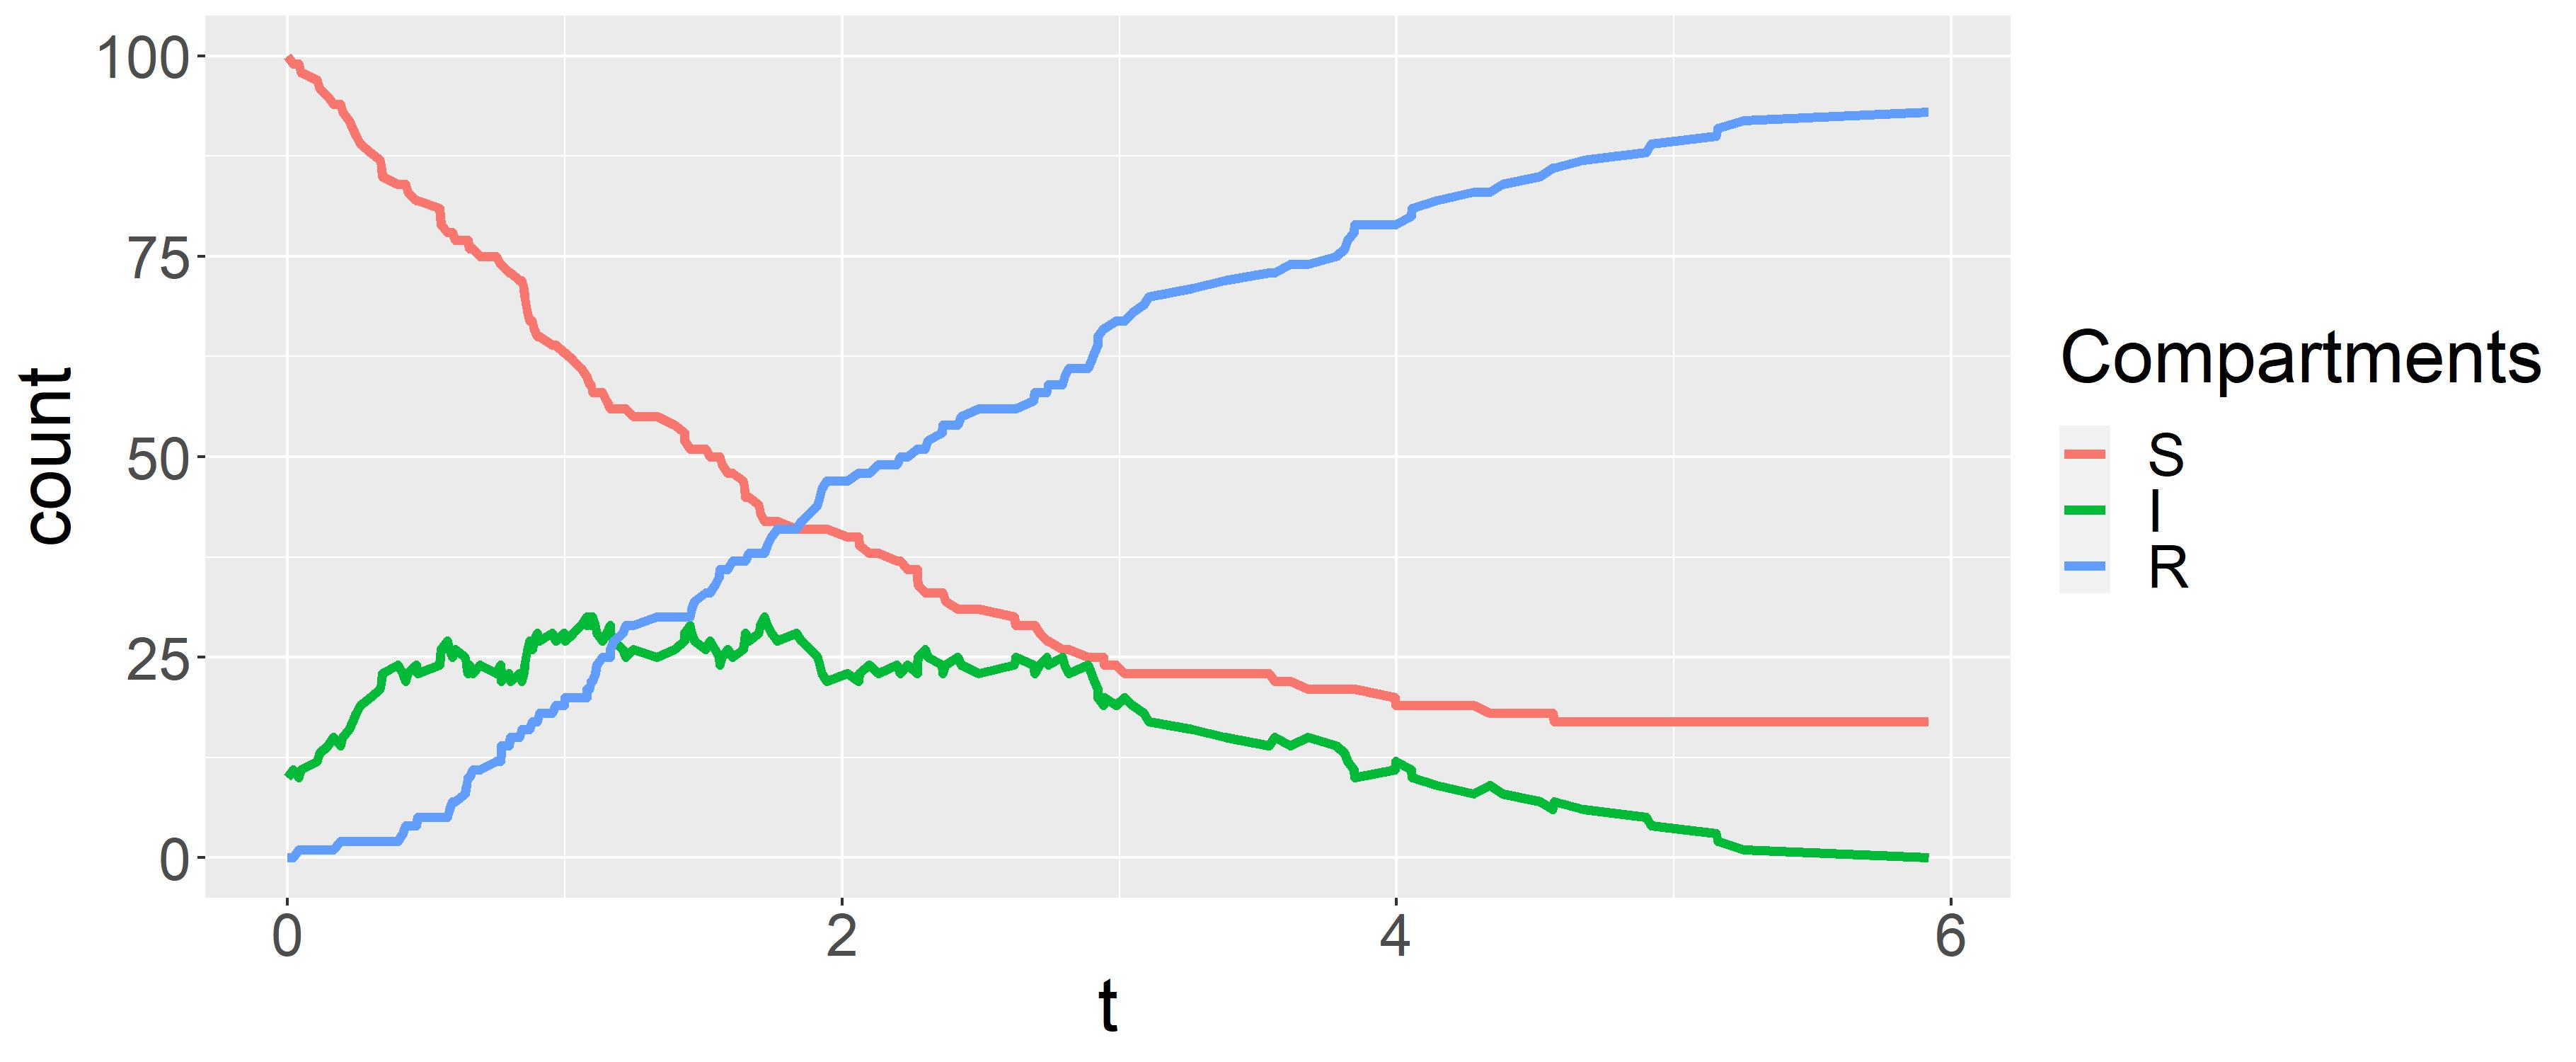
\includegraphics[scale = 0.2]{E3_S0=100_trajectories}
			\caption{Compartment trajectories of a stochastic SIR process.}
		\end{figure}
	\end{itemize}
	
\end{frame}


\begin{frame} \frametitle{Stochastic SIR Model}  

	Consider the agent-based epidemic process $\left\lbrace \X(t), t>0\right\rbrace$, 
	$$\X(t) = (X_1(t), \dots, X_n(t)) \in \{s, i, r\}^n$$
	where the agent-level subprocess
	$$ X_j(t) = 
	\begin{cases}
		s, & t \in (0, \tau^I_j) \\
		i, & t \in (\tau^I_j, \tau^R_j) \\
		r, & t \in (\tau^R_j, \infty)
	\end{cases}
	,\quad \iton
	$$
	denotes the compartment of individual $j$ over time.
	
\end{frame}


\begin{frame} \frametitle{Stochastic SIR Model}  
	
	\begin{itemize}
		\item Three common assumptions:
		\begin{itemize}
			\item Homogeneously mixing population: contacts between pairs of individuals follow independent Poisson. processes with rate $\beta$,
			\item Markovian assumption: iid exponentially distributed infectious periods with rate $\gamma$.
			\item Closed population.
		\end{itemize}
	\vfill
		\item These assumptions yield a \textit{Markov} process characterized by the transition rates			
			$
			\lambda_{\x, \x'} = 
			\begin{cases}
				\beta I(t), & \x \text{ and } \x' \text{ only differ at position } j \text{ with } x_j = s \text{ and } x_j' = i, \\
				\gamma, & \x \text{ and } \x' \text{ only differ at position } j \text{ with } x_j = i \text{ and } x_j' = r, \\
				0, & \text{otherwise.}
			\end{cases}
			$
	\end{itemize}
\end{frame}



\begin{frame} \frametitle{SIR -- Population-based Formulation} 
	
	The agent-based formulation is equivalent to the more typical population-based formulation with
	$$W(t) = \left( S(t), I(t), R(t)\right)  \in \{0, 1, \cdots, n\}^3$$
	and 	
	$
	\lambda_{(S, I, R), (S', I', R')} = 
	\begin{cases}
		\beta S(t) I(t), & (S', I', R') = (S - 1, I + 1, R)\\
		\gamma I(t)    , & (S', I', R') = (S, I - 1, R + 1)\\
		0, & \text{otherwise.}
	\end{cases}
	$
	\vfill
	The agent-based formulation will allow us to
	\begin{itemize}
		\item leave the Markovian framework,
		\item jointly propose latent data in our DA-MCMC.
	\end{itemize}
	
\end{frame}




\begin{frame} \frametitle{Inference}  

	The stochastic SIR process has a closed-form likelihood 
	\begin{align*}
		L(\theta; \X)
		& = \prod_{j \in \mathcal{I}} \beta I(\tau^I_j) \prod_{k \in \mathcal{R}} \gamma \exp\left\lbrace - \int_{0}^{t_{end}}\beta S(t)I(t) + \gamma I(t) dt \right\rbrace \\
		\label{eq:cdl}
		& = \beta^{n_I} \gamma^{n_R}\prod_{j \in \mathcal{I}} I(\tau^I_j) \exp\left\lbrace - \beta \int_{0}^{t_{end}} S(t)I(t) - \gamma \int_{0}^{t_{end}} I(t) dt \right\rbrace
	\end{align*}
	where
	\begin{itemize}
		\item $\mathcal{I} = \{j: \tau^I_j \in (0, t_{end}]\}$ and $\mathcal{R} = \{j: \tau^R_j \in (0, t_{end}]\}$,
		\item $n_I = |\mathcal{I}|$ and $n_R = |\mathcal{R}|$
	\end{itemize}
			
\end{frame}





\begin{frame} \frametitle{Inference}	
	Closed-form MLE:
	$$
	\hat{\beta} = \dfrac{n_I}{ \int_{0}^{t_{end}} S(t)I(t)dt}, \qquad \hat{\gamma} = \dfrac{n_R}{ \int_{0}^{t_{end}} I(t)dt},
	$$
	\begin{itemize}
		\item the integrals correspond to finite sums ($I(t)$ and $S(t)$ are constant between event times),
	\end{itemize}
	and gamma conjugacy:
	\begin{equation*}
		\beta \sim G(a_{\beta}, b_{\beta}), \qquad \gamma \sim G(a_{\gamma}, b_{\gamma}),
	\end{equation*}
	\begin{align*}
		\beta | \X & \sim G\left( a_{\beta} + n_I , b_{\beta} + \int_{0}^{t_{end}} I(t)S(t) dt\right), \\
		\gamma | \X & \sim G\left( a_{\gamma} + n_R, b_{\gamma} + \int_{0}^{t_{end}} I(t) dt\right)
	\end{align*}

\end{frame}



\begin{frame} \frametitle{Inference - Reparameterization}  
	
The SIR likelihood can also be parameterized in terms of $\tilde{\theta} = (\beta, R_0)$ with $R_0 = S(0) \beta / \gamma$
which has the semi-conjugate prior
\begin{equation*}
	\beta \sim G(a_{\beta}, b_{\beta}), \qquad R_0 \sim IG(a_{R}, b_{R})
\end{equation*}
\begin{align*}
\beta | \X, R_0 & \sim G\left( a_{\beta} + n_I + n_R, b_{\beta} + \int_{0}^{t_{end}} S(t)I(t) dt + \frac{S(0)}{R_0} \int_{0}^{t_{end}} I(t) dt\right) \\
R_0 | \X, \beta & \sim IG\left( a_{R} + n_R, b_{R} + \beta S(0) \int_{0}^{t_{end}} I(t) dt\right)
\end{align*}
$\Rightarrow$ Gibbs sampler to explore $\pi(\tilde{\theta}|\X)$.
\end{frame}


\begin{frame} \frametitle{Inference - Reparameterization}  
	
	\begin{figure}
	\centering
	\begin{subfigure}[b]{0.49\textwidth}
		\centering
		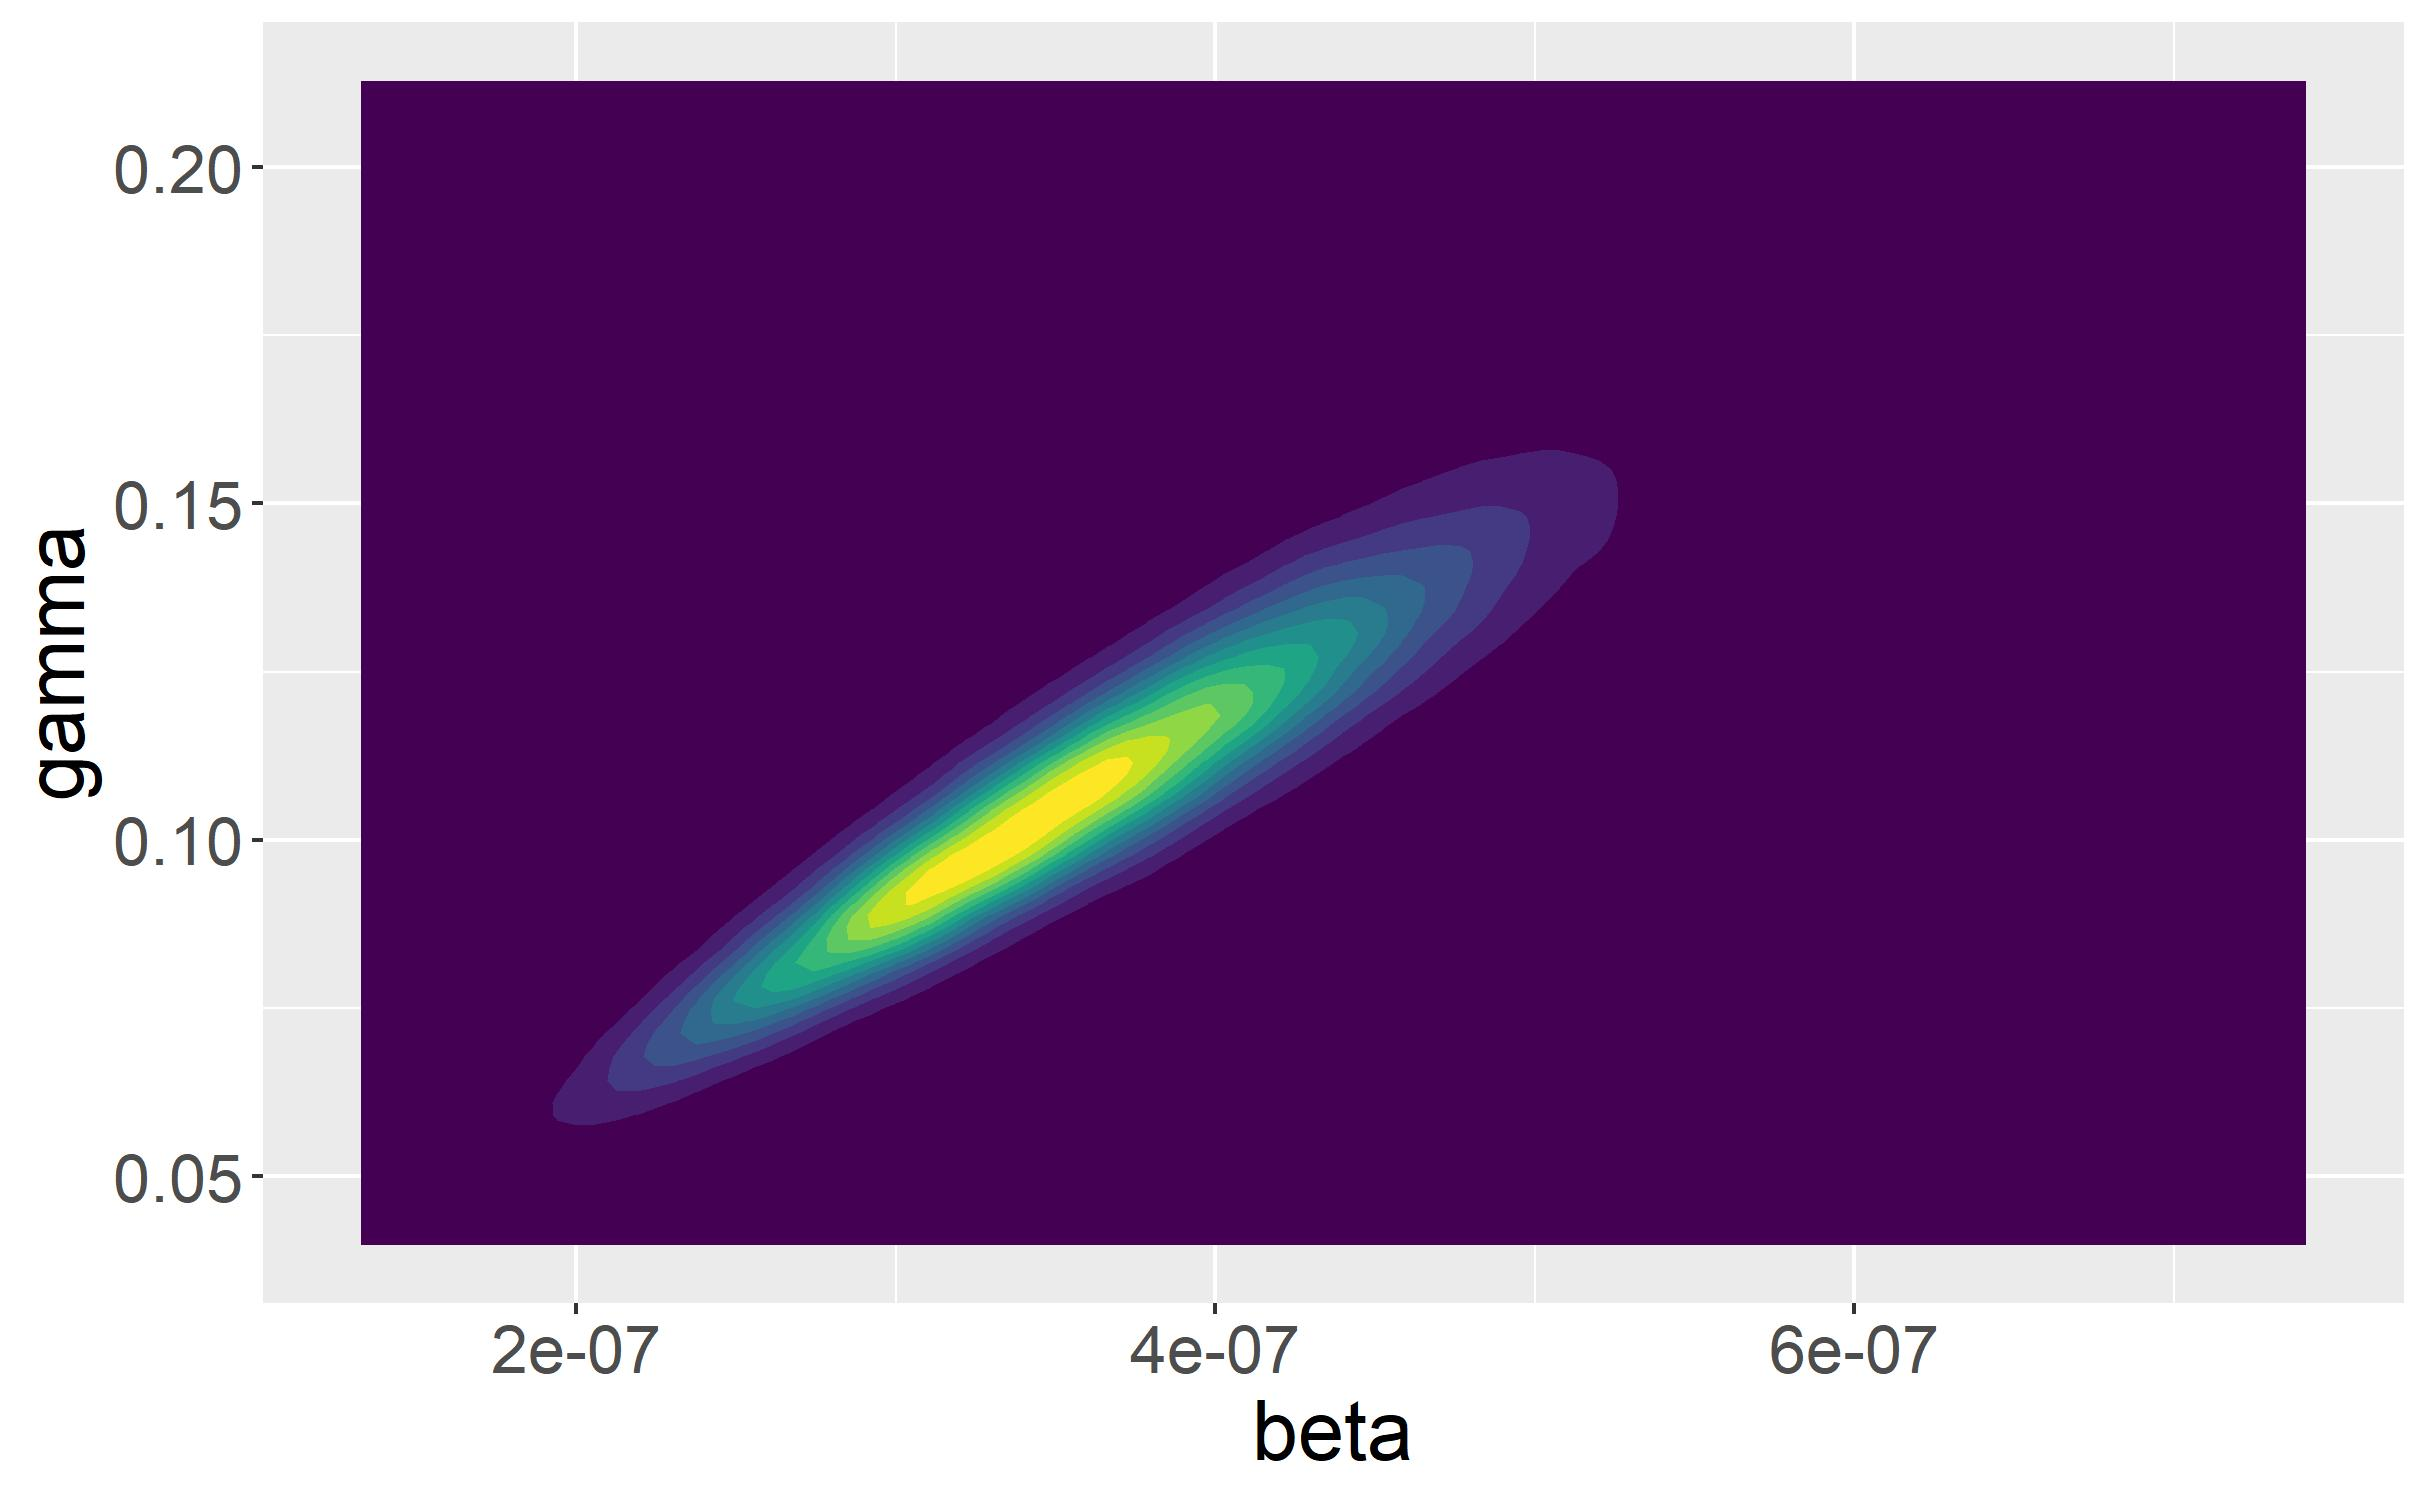
\includegraphics[width=\textwidth]{E5_beta_gamma_bi_dens}
		\caption{$\theta = (\beta, \gamma)$}
	\end{subfigure}
	\hfill
	\begin{subfigure}[b]{0.49\textwidth}
		\centering
		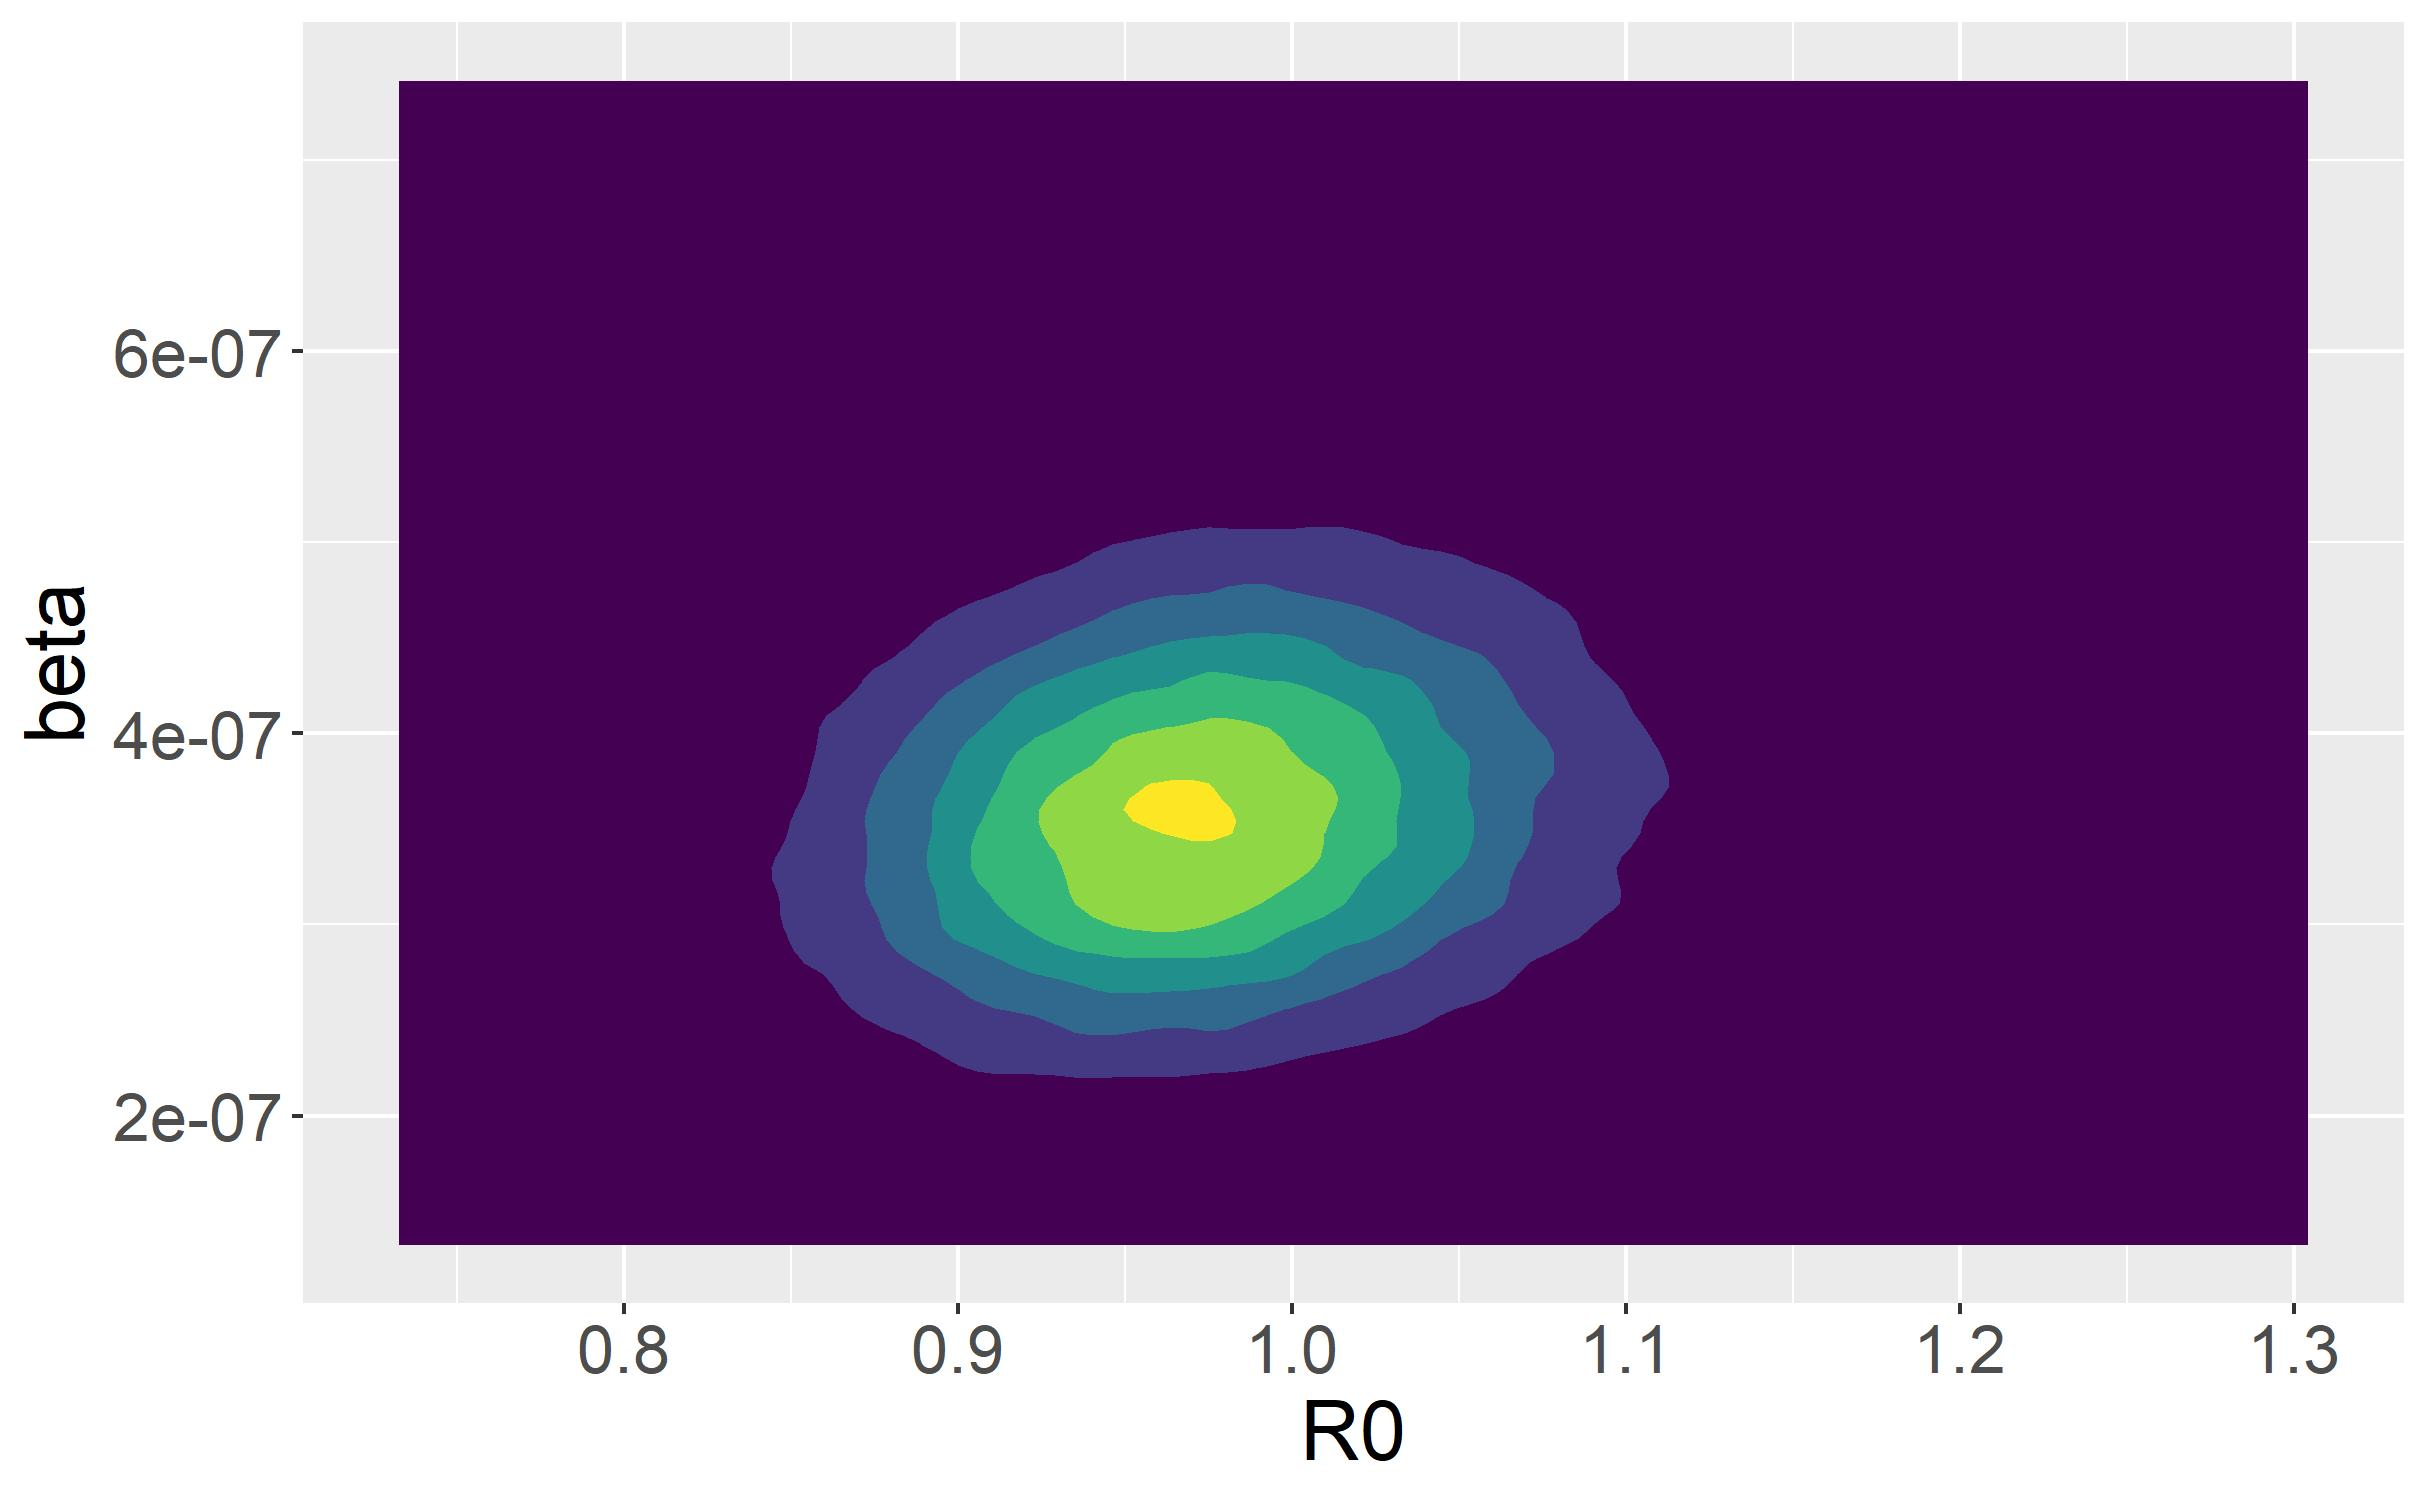
\includegraphics[width=\textwidth]{E5_R0_beta_bi_dens}
		\caption{$\tilde{\theta} = (\beta, R_0)$}
	\end{subfigure}
	\caption{Joint posterior given partial data under different parameterizations.}
\end{figure}

\end{frame}



\begin{frame} \frametitle{Partial Data - Incidence Data for Infection}  
	
	\begin{itemize}
		\item In practice, the process is never completely observed.
		\item In my research, I consider \textit{incidence data for infections}
		\item Given times $t_{0:K}$, the observed data are $\Y = I_{1:K}$ where 
		$$I_k = \#\{\tau^I_j \in (t_{k-1}, t_k]\}$$
		is the number of infections during the $k$th interval.
		\item E.g.\ weekly infection counts.
		\item Motivated by the 2013-2016 Ebola pandemic in Western Africa.
	\end{itemize}
\end{frame}

\begin{frame} \frametitle{Intractable Partial Likelihood}
	
	The partial data likelihood
	\begin{equation*}
	L(\theta; \Y) = \pi(\theta) \int_{\chi_\x} L(\theta; \x) \delta_{\Y}(\x) d\x,
	\end{equation*}
	where $\delta_{\Y}(\x) = 1$ if $\Y$ is compatible with the infection times in $\x$ and $0$ otherwise,
	is intractable.
	
\end{frame}


\begin{frame} \frametitle{Prior Work}
	
	\begin{itemize}
		\item Direct method to compute $L(\theta; Y)$ (Ho et al., 2018)
		\begin{itemize}
			\item Prohibitively slow.
		\end{itemize}
		\item Approximate likelihood (Fintzi et al., 2020)
		\begin{itemize}
			\item Assumptions questionable in small populations.
		\end{itemize}
		\item Particle filtering (King - 2015)
		\begin{itemize}
			\item Often degenerates.
		\end{itemize}
		\item DA-MCMC with RJ (Gibson and Renshaw - 1998)
		\begin{itemize}
			\item Single-site update MH step.
		\end{itemize}
		\item DA-MCMC with MH (Fintzi et al., 2017)
		\begin{itemize}
			\item Single-site update MH step.
		\end{itemize}
		\item DA-MCMC with Gibbs (Touloupou et al., 2020)
		\begin{itemize}
			\item Discrete time, single-site update Gibbs step.
			\item No likelihood evaluation (expensive step), but FFBS.
		\end{itemize}
	\end{itemize}
	
\end{frame}

\begin{frame} \frametitle{DA-MCMC}  
	
	The closed-form likelihood $L(\theta; \X)$ and its (semi) conjugacy suggests using Data-Augmentation MCMC:
		\begin{itemize}
			\item Construct latent $\Z = \left\lbrace (z^I_j, z^R_j)\right\rbrace_{j=1}^{n}$ and explore $\pi(\theta, \Z|\Y)$.
			\item Naive approach: Gibbs sampler
			\begin{itemize}
				\item $\theta|\Y, \Z$ -- (semi) conjugacy
				\item $\Z|\Y,\theta$ -- prohibitively difficult
			\end{itemize}
		\end{itemize}
	\vfill
	Existing DA-MCMC approaches substitute the difficult Gibbs step $\Z|\Y,\theta$ with a simpler single-site-update MH step.	
	\begin{itemize}
		\item The resulting Markov chain is very sticky.
		\item Limited to populations with $n<1000$ individuals.
	\end{itemize}
	\vfill
	We propose \textbf{a DA-MCMC algorithm in which the entire latent data $\Z$ are jointly proposed in a MH step}.
		
\end{frame}

\begin{frame} \frametitle{Piece-wise decoupled SIR}
		
	Main idea of our DA-MCMC: use a \textit{surrogate} process to generate latent data $\Z^\star$ compatible with the observed data $\Y$ and accept/reject $\Z^\star$ in a MH step.
	\vfill
	To generate $\Z^\star$ compatible with $\Y = I_{1:K}$, proceed one interval at a time.
	\begin{itemize}
		\item Generate the $I_k$ infection times in $(t_{k-1}, t_k)$ using some procedure, e.g.\ iid $U(t_{k-1}, t_k)$.
		\item Generate the removal times of these inviduals by adding an exponential RV to their infection times.		
	\end{itemize}
\vfill
	We want to generate the infection times using a procedure that is as close as possible to the SIR.
	
\end{frame}


\begin{frame} \frametitle{Piece-wise decoupled SIR}
	
	Under the SIR, the \textit{population} infection rate $\mu_{pop}(t) = \beta I(t) S(t)$ changes after every event. Consider two approximations:
	\begin{enumerate}
		\item Let $\tilde{\tilde{\mu}}_{pop}$ be constant over each interval $[t_{k-1}, t_k)$:
		$$\tilde{\tilde{\mu}}_{pop}(t) := \mu_{pop}(t_{k-1}) = \beta S(t_{k-1})I(t_{k - 1}), \quad t \in [t_{k - 1}, t_k).$$
		The $I_k$ infection times follow a Poisson process (iid uniform).
		
		\item Let $\tilde{\mu}_{pop}$ be decoupled of $I(t)$ only (PD-SIR).
		$$\tilde{\mu}_{pop}(t) := \beta S(t)I(t_{k - 1}), \quad t \in [t_{k - 1}, t_k).$$
		\begin{itemize}
			\item The corresponding \textit{individual} infection rate is $\tilde{\mu}(t) :=\dfrac{\tilde{\mu}_{pop}(t)}{S(t)} = \beta I(t_{k - 1}) = \mu_k$ is piece-wise constant.
			\item The compartment $S(t)$ follows a linear death process (LDP) where infections correspond to deaths.
		\end{itemize}
	\end{enumerate}
	
\end{frame}


\begin{frame}
	
	\begin{figure}
		\centering
		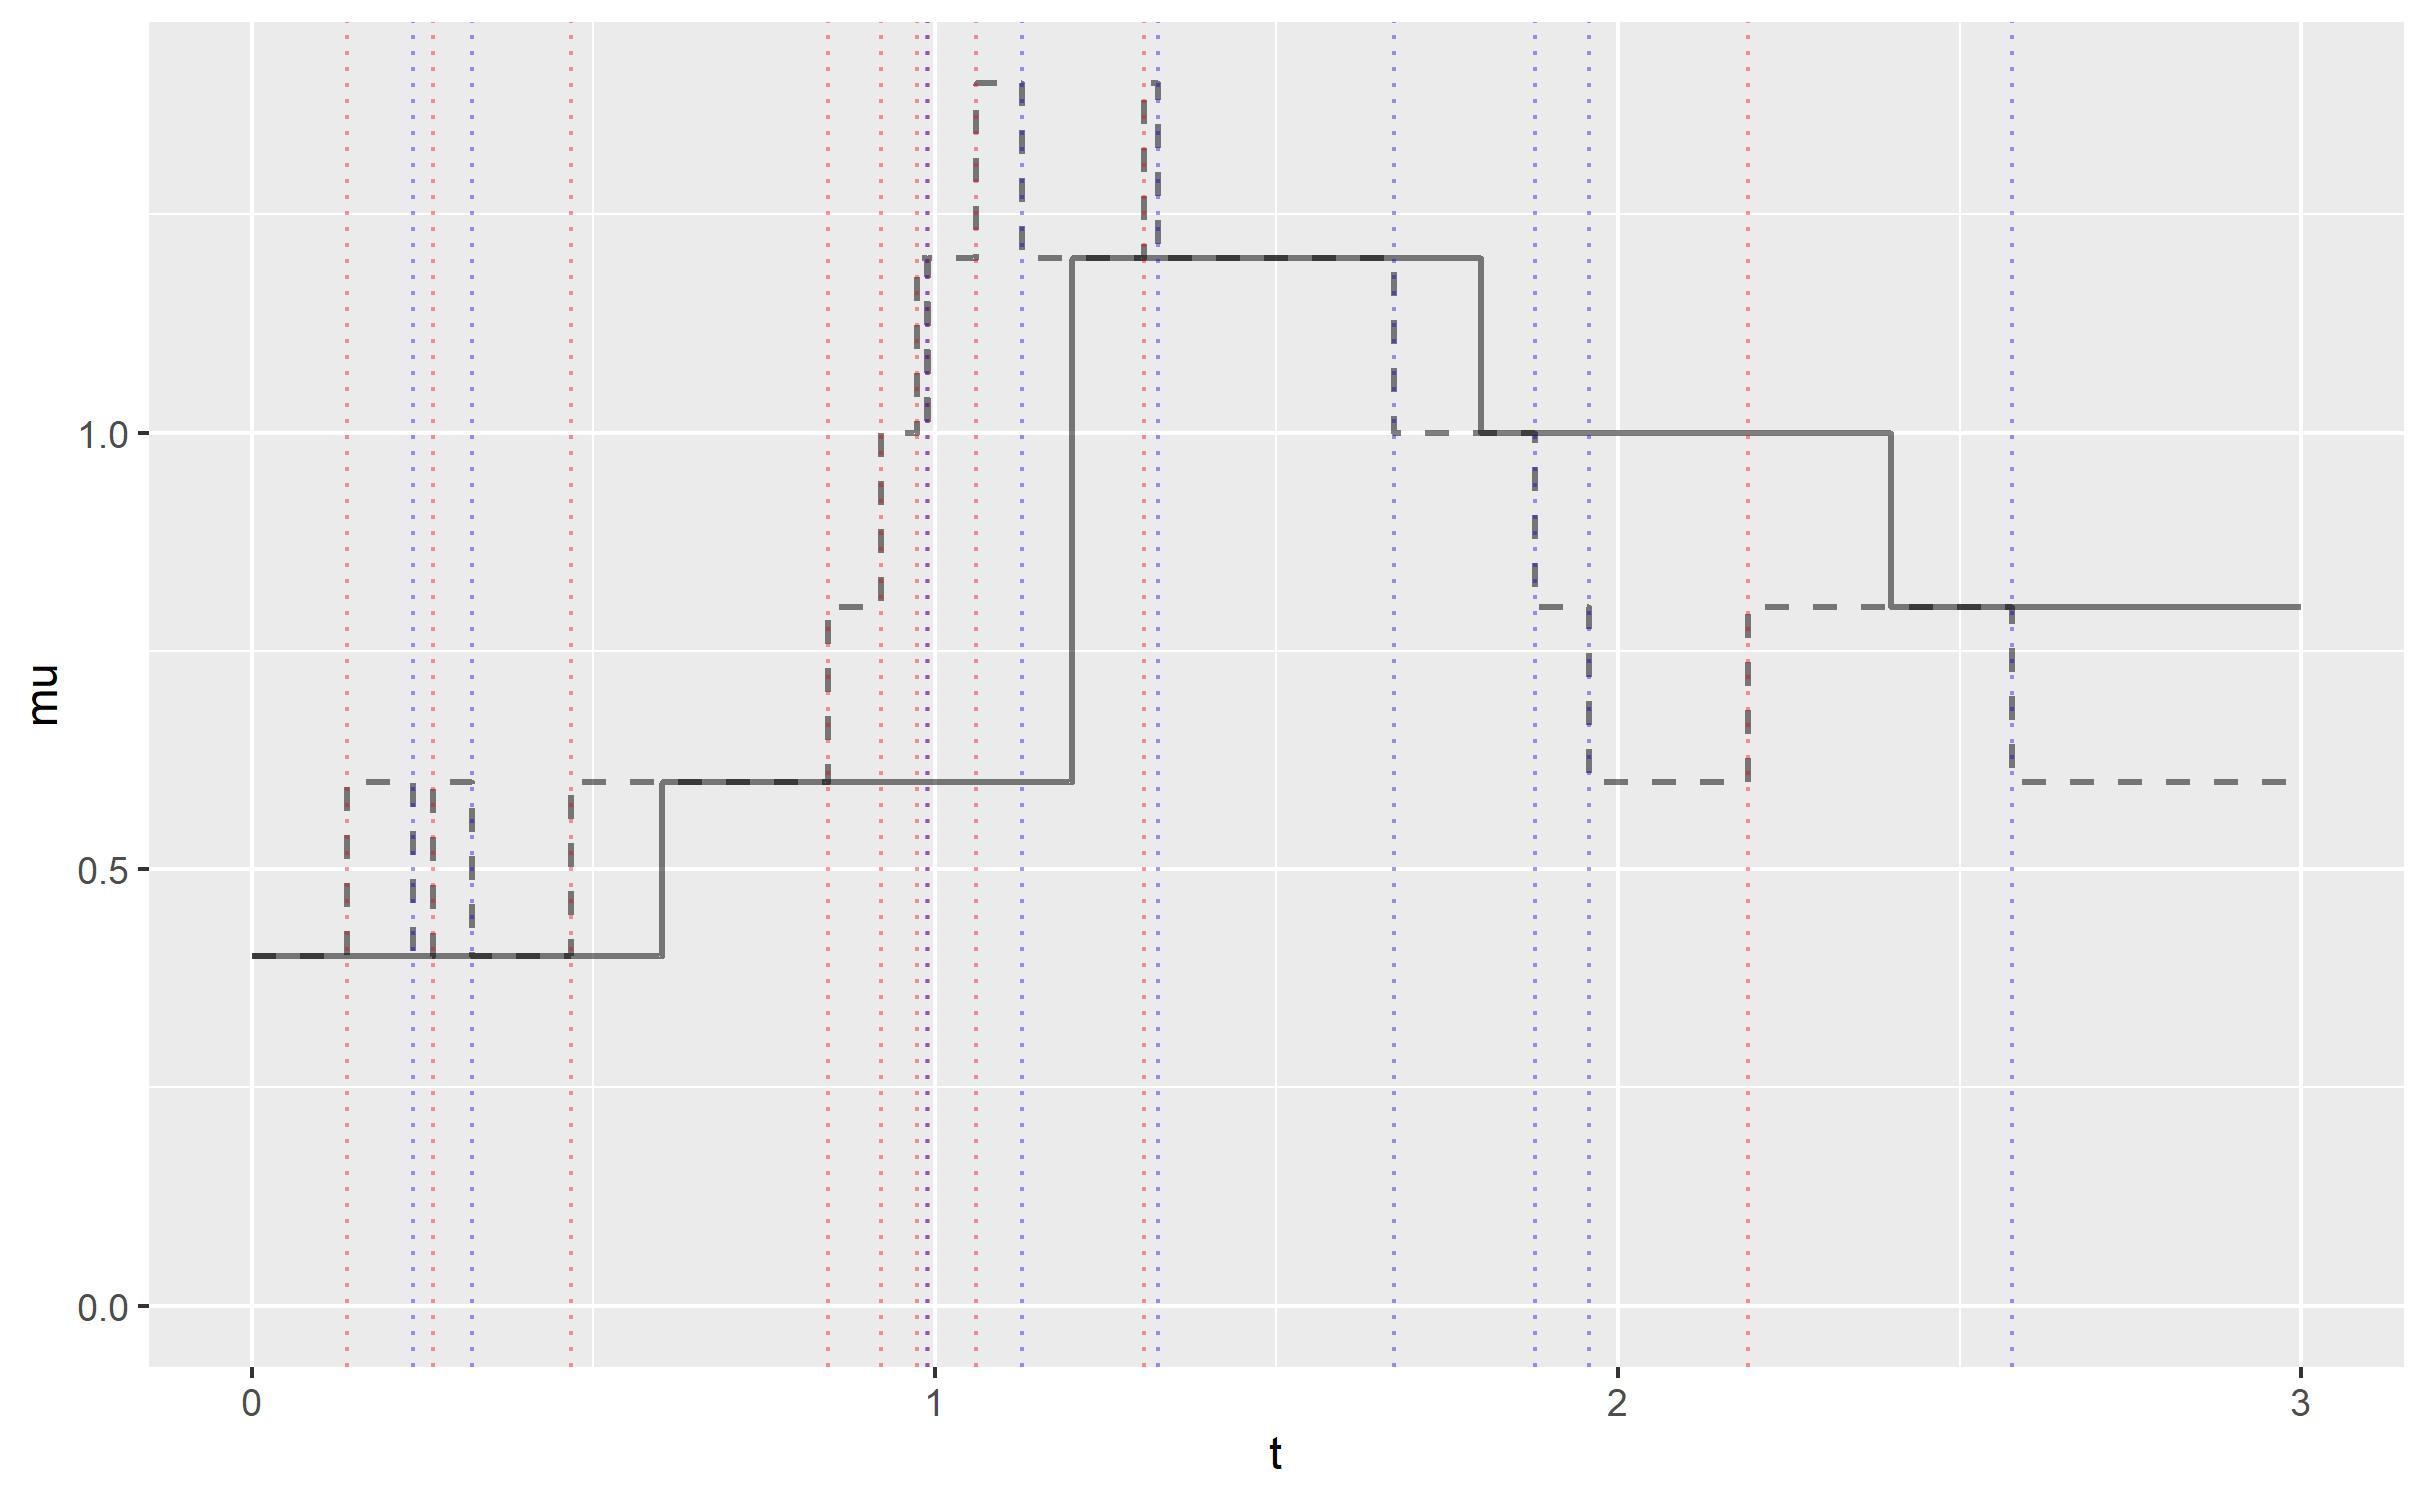
\includegraphics[scale = 0.4]{infection_rate_SIR_PDSIR}
		\caption{Individual infection rate under the SIR (dashed) and PD-SIR (solid) processes. Small population ($n = 10$) and $t_{0:3} = (0, 0.2, 0.4, 0.6)$.}
	\end{figure}			
\end{frame}


\begin{frame}
	
	\begin{figure}
		\centering
		\begin{subfigure}[b]{0.49\textwidth}
			\centering
			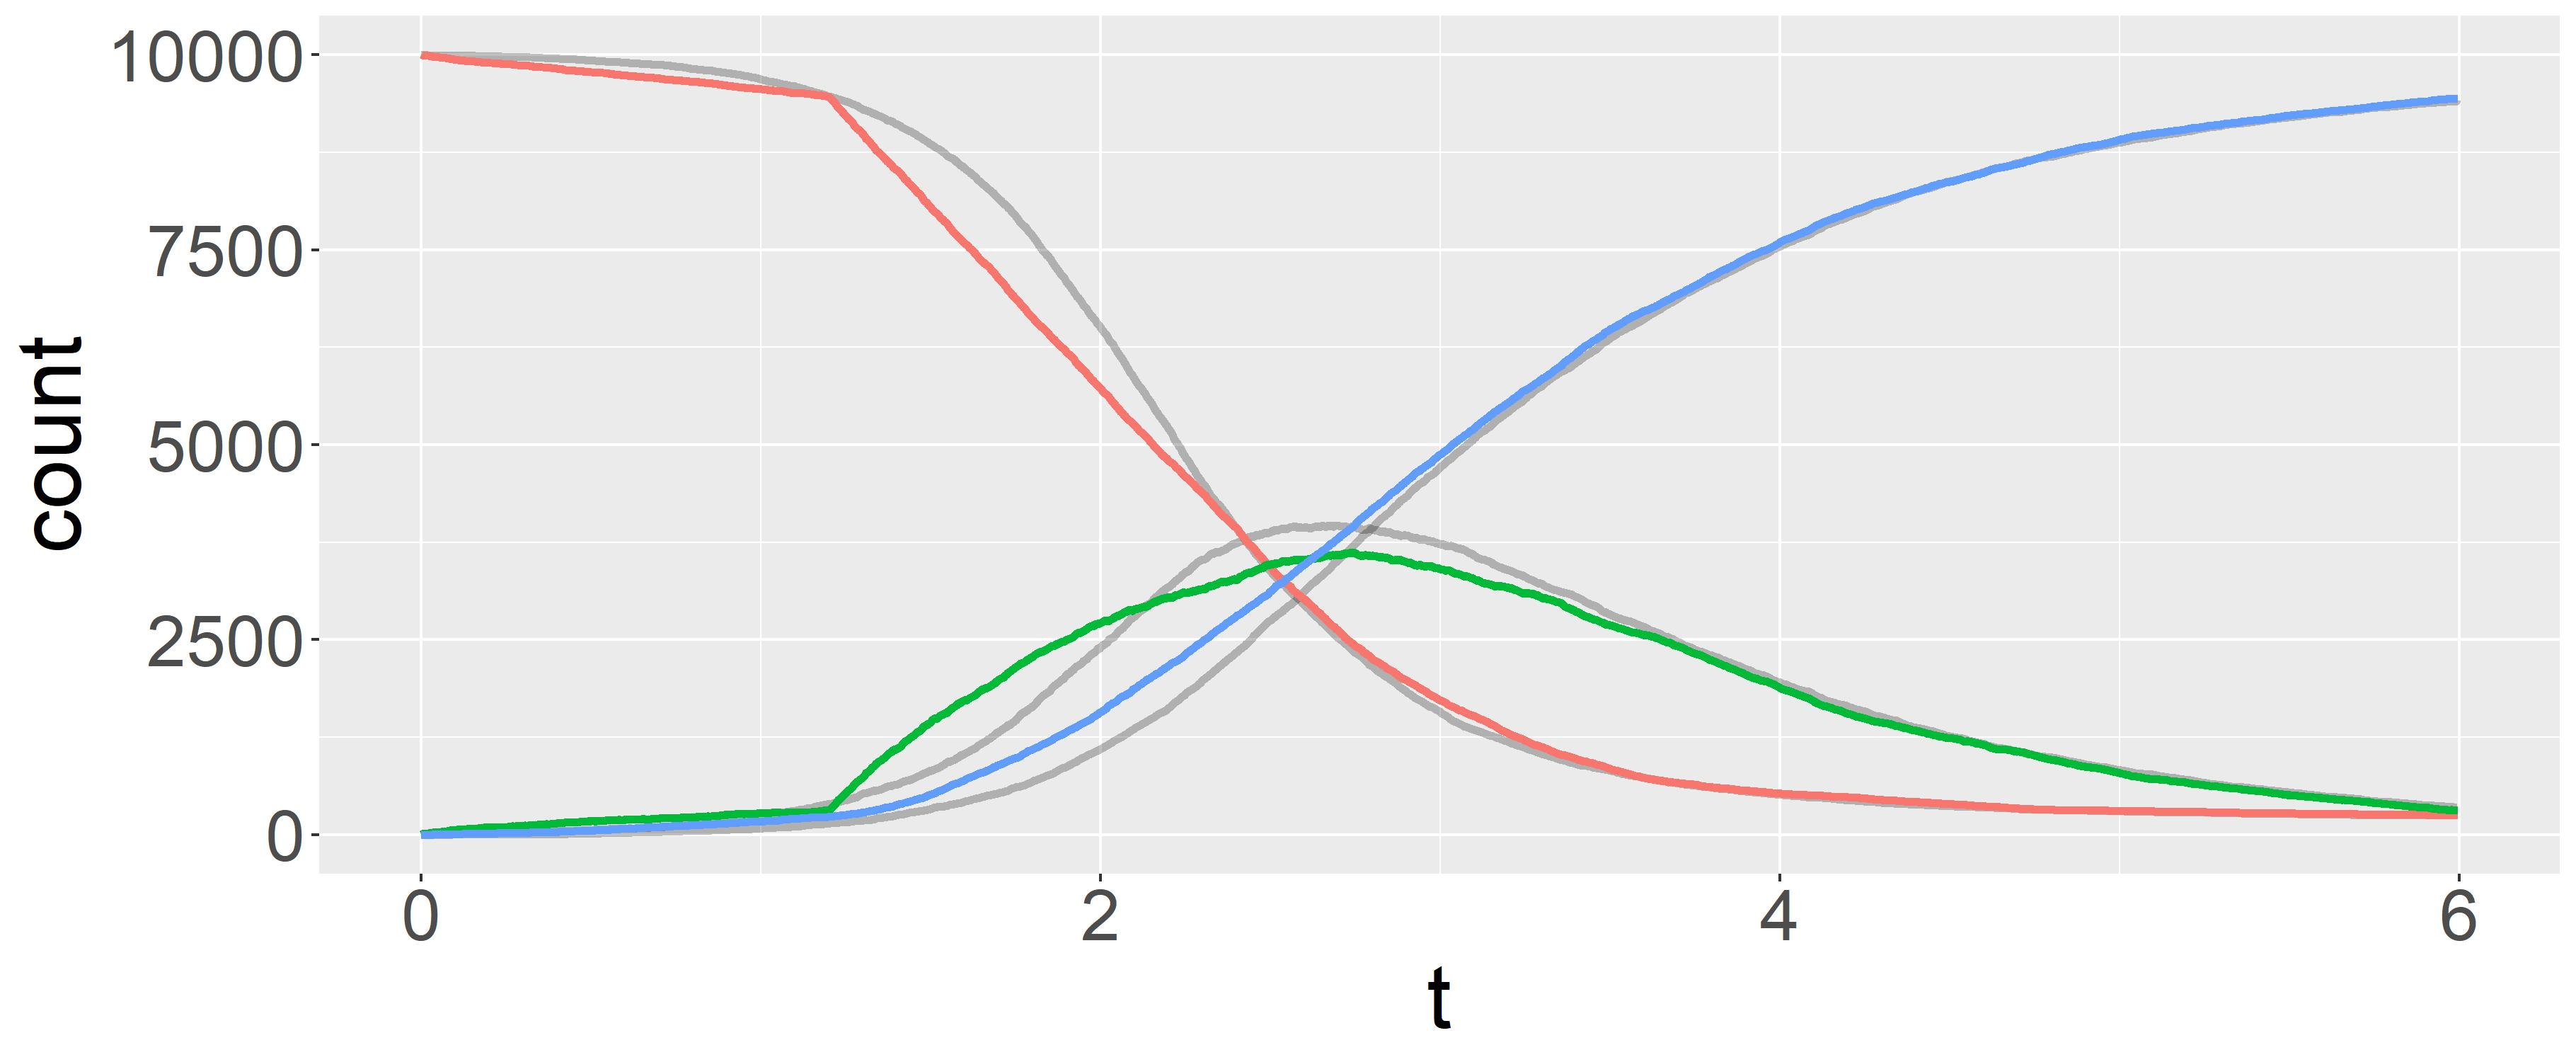
\includegraphics[width=\textwidth]{E2_K5.jpeg}
			\caption{$K=5$}
		\end{subfigure}
		\hfill
		\begin{subfigure}[b]{0.49\textwidth}
			\centering
			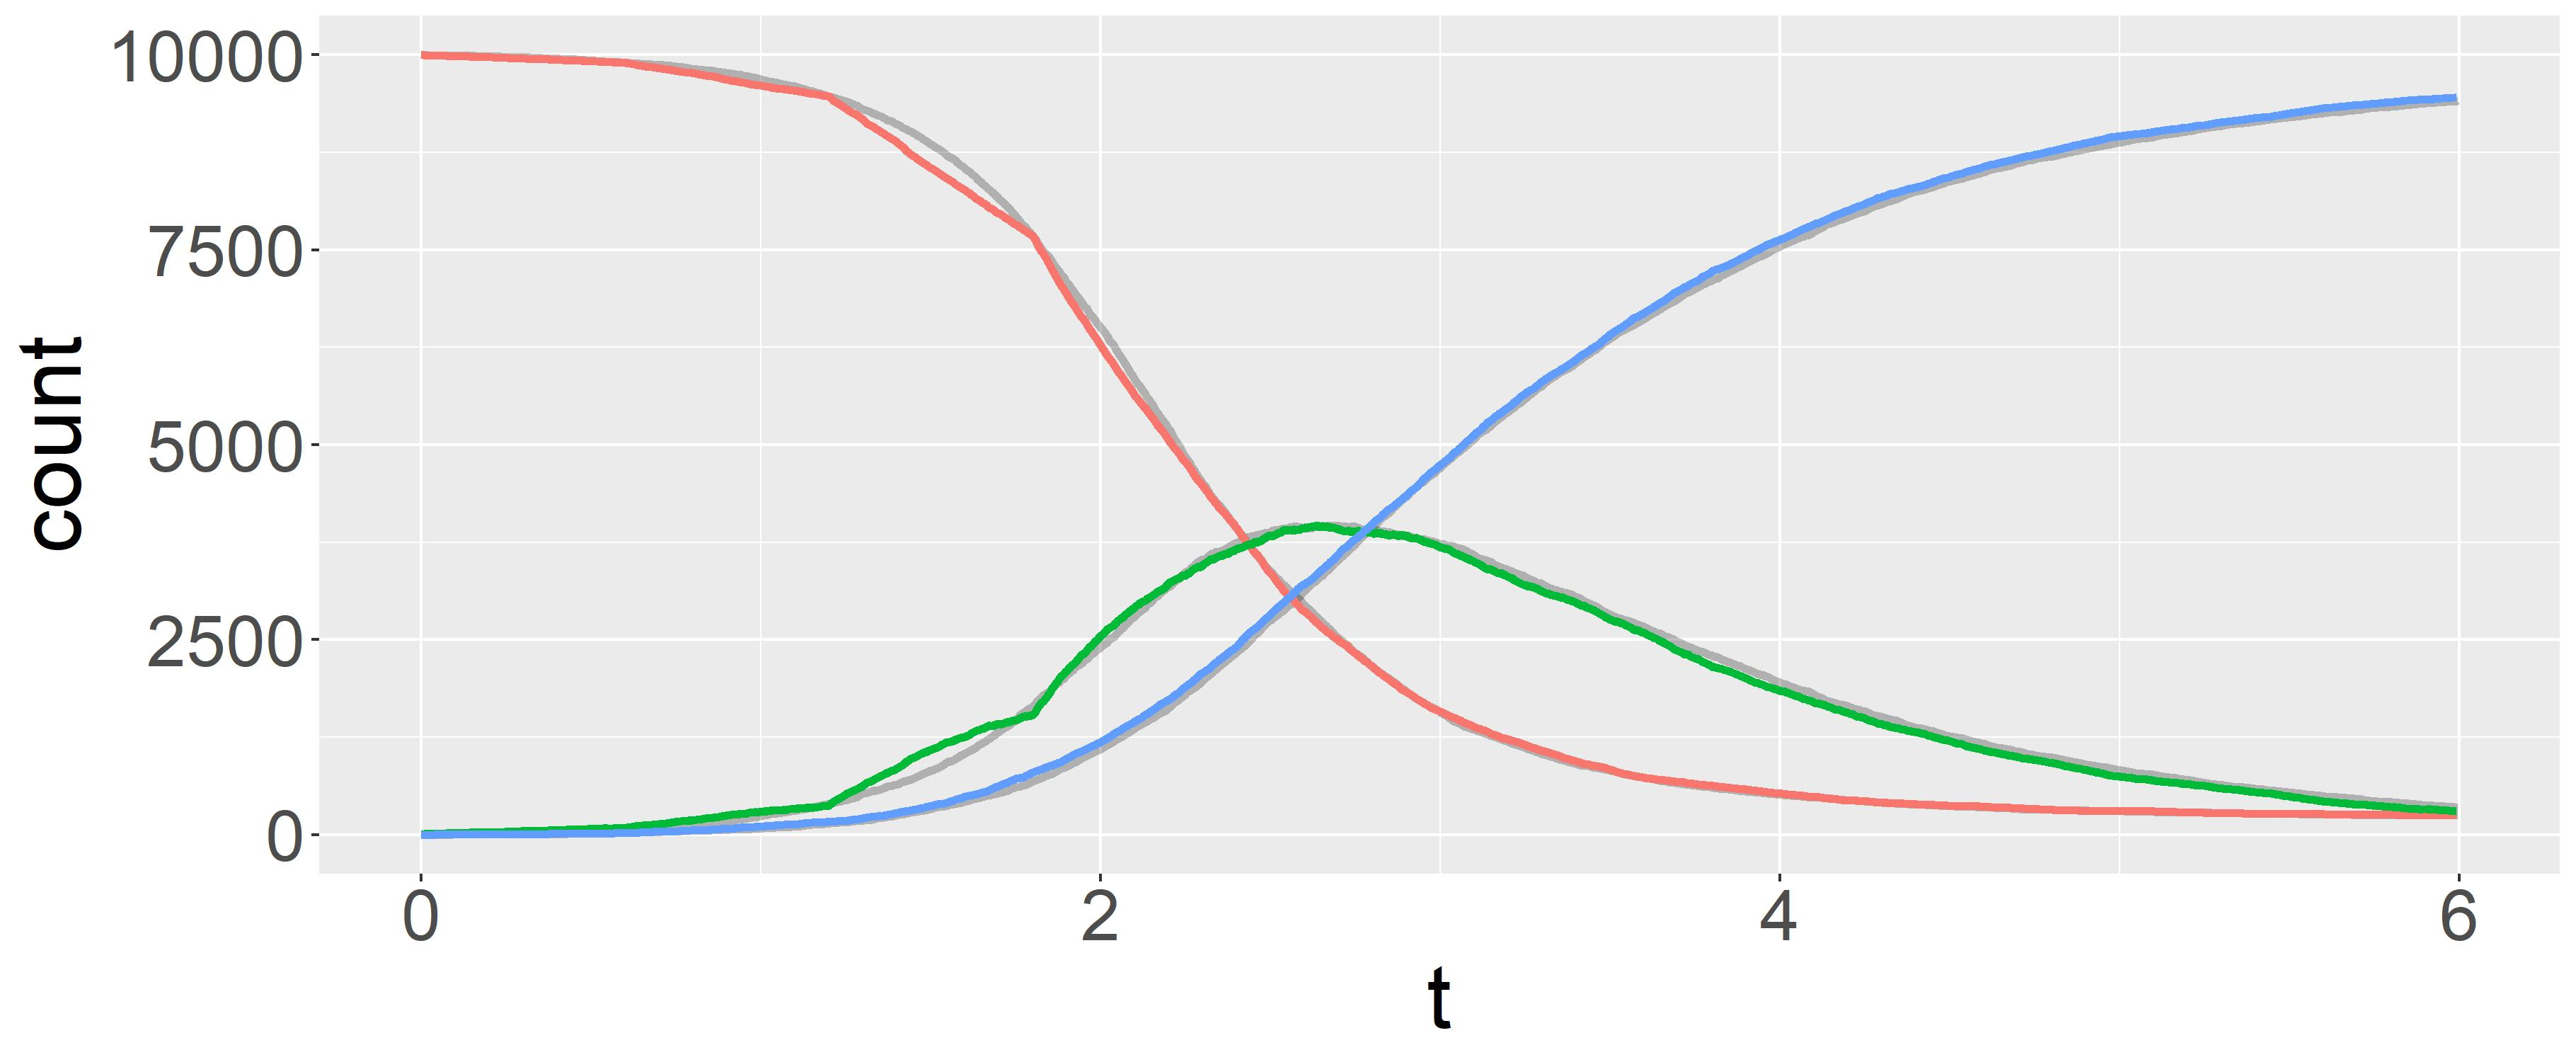
\includegraphics[width=\textwidth]{E2_K10.jpeg}
			\caption{$K=10$}
		\end{subfigure}
		\\
		\begin{subfigure}[b]{0.49\textwidth}
			\centering
			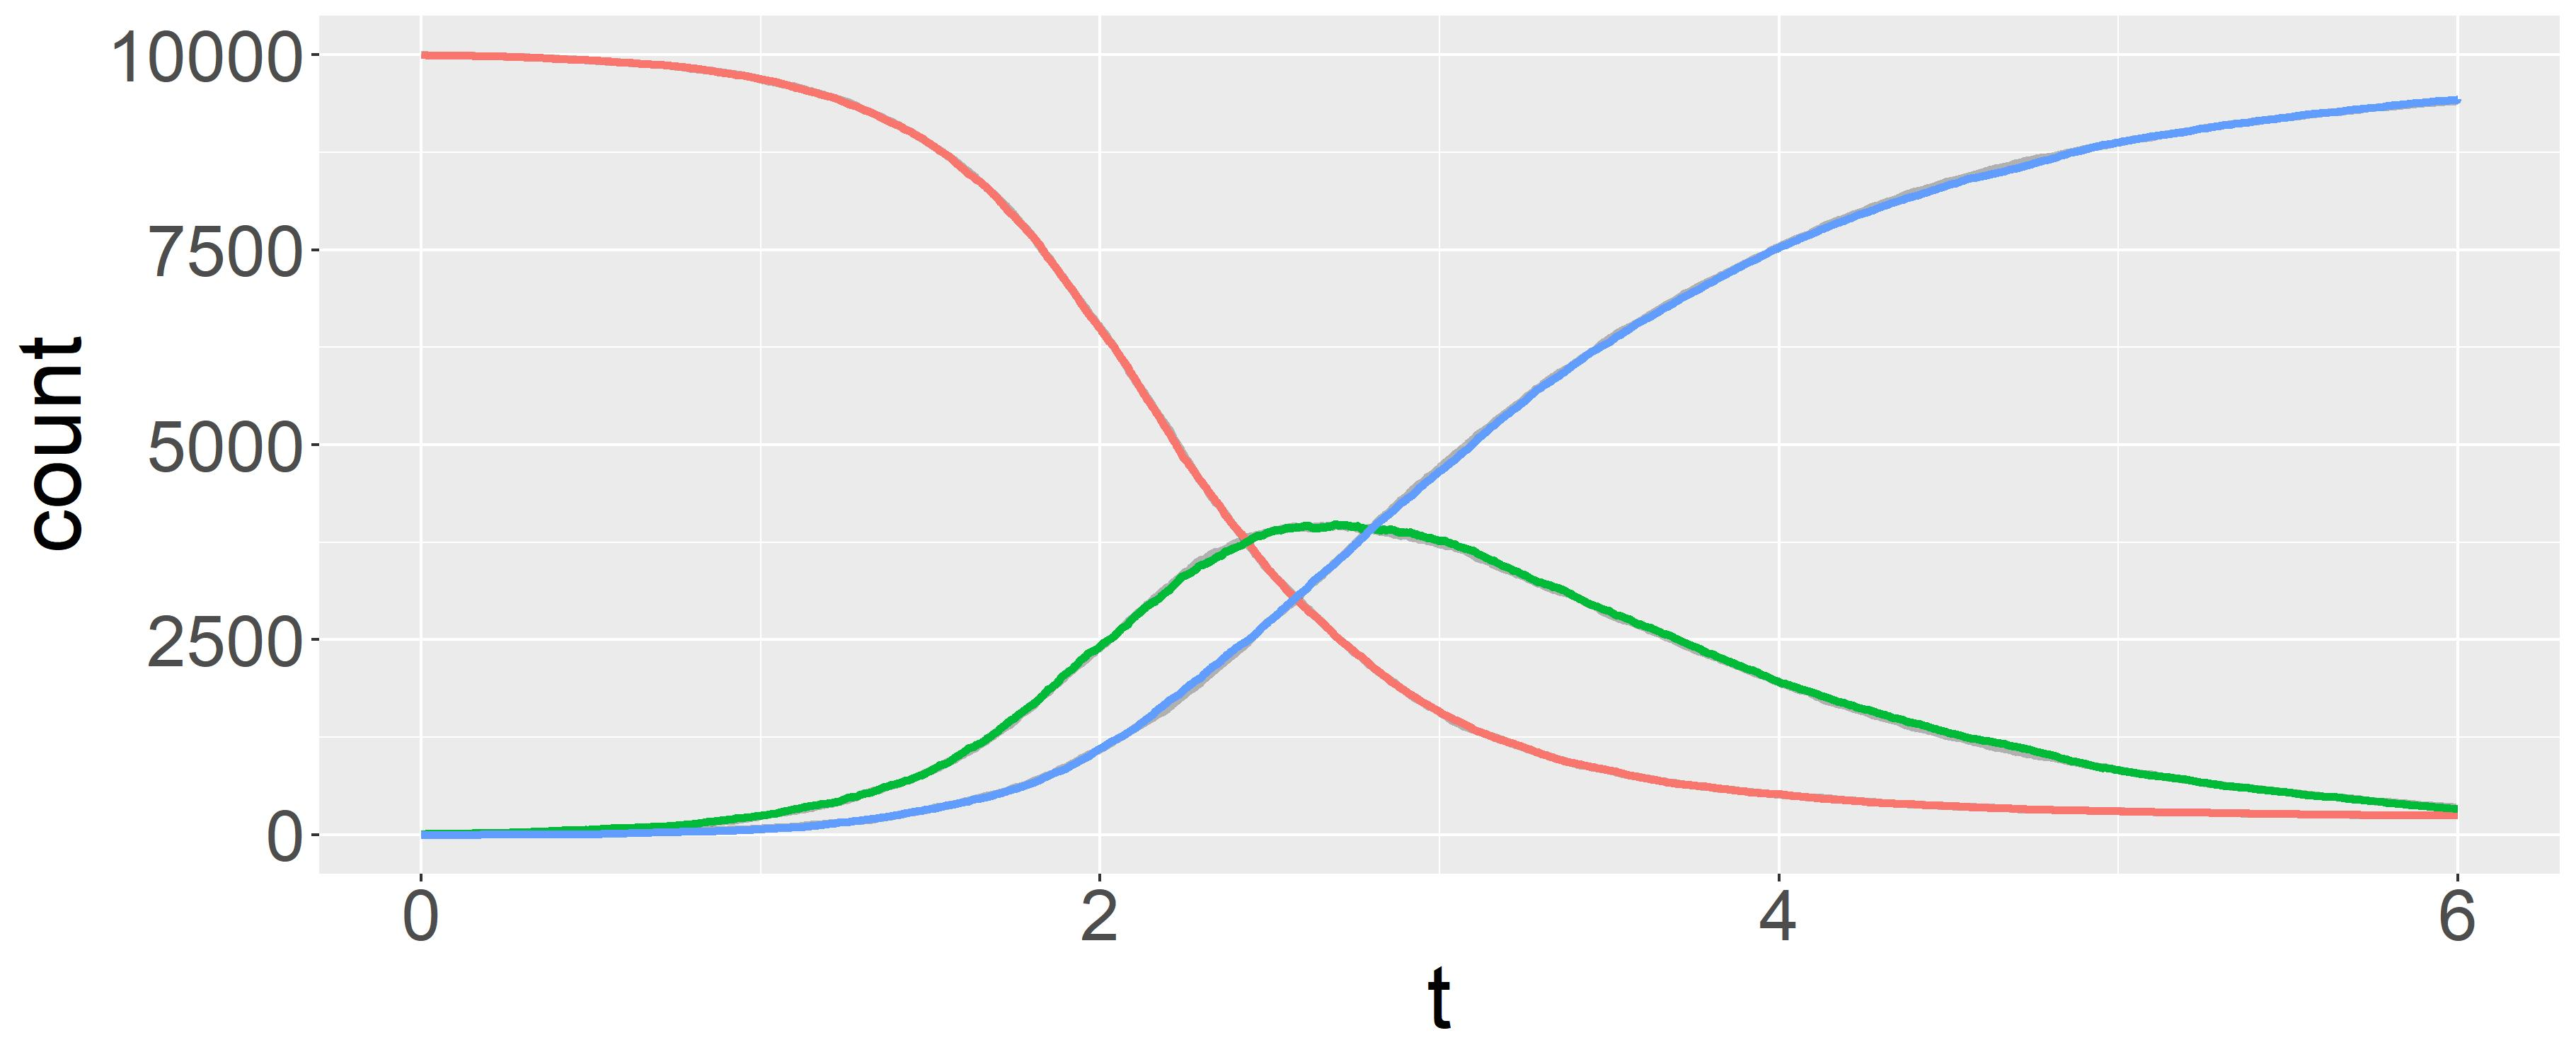
\includegraphics[width=\textwidth]{E2_K50.jpeg}
			\caption{$K=50$}
		\end{subfigure}
		\hfill
		\begin{subfigure}[b]{0.49\textwidth}
			\centering
			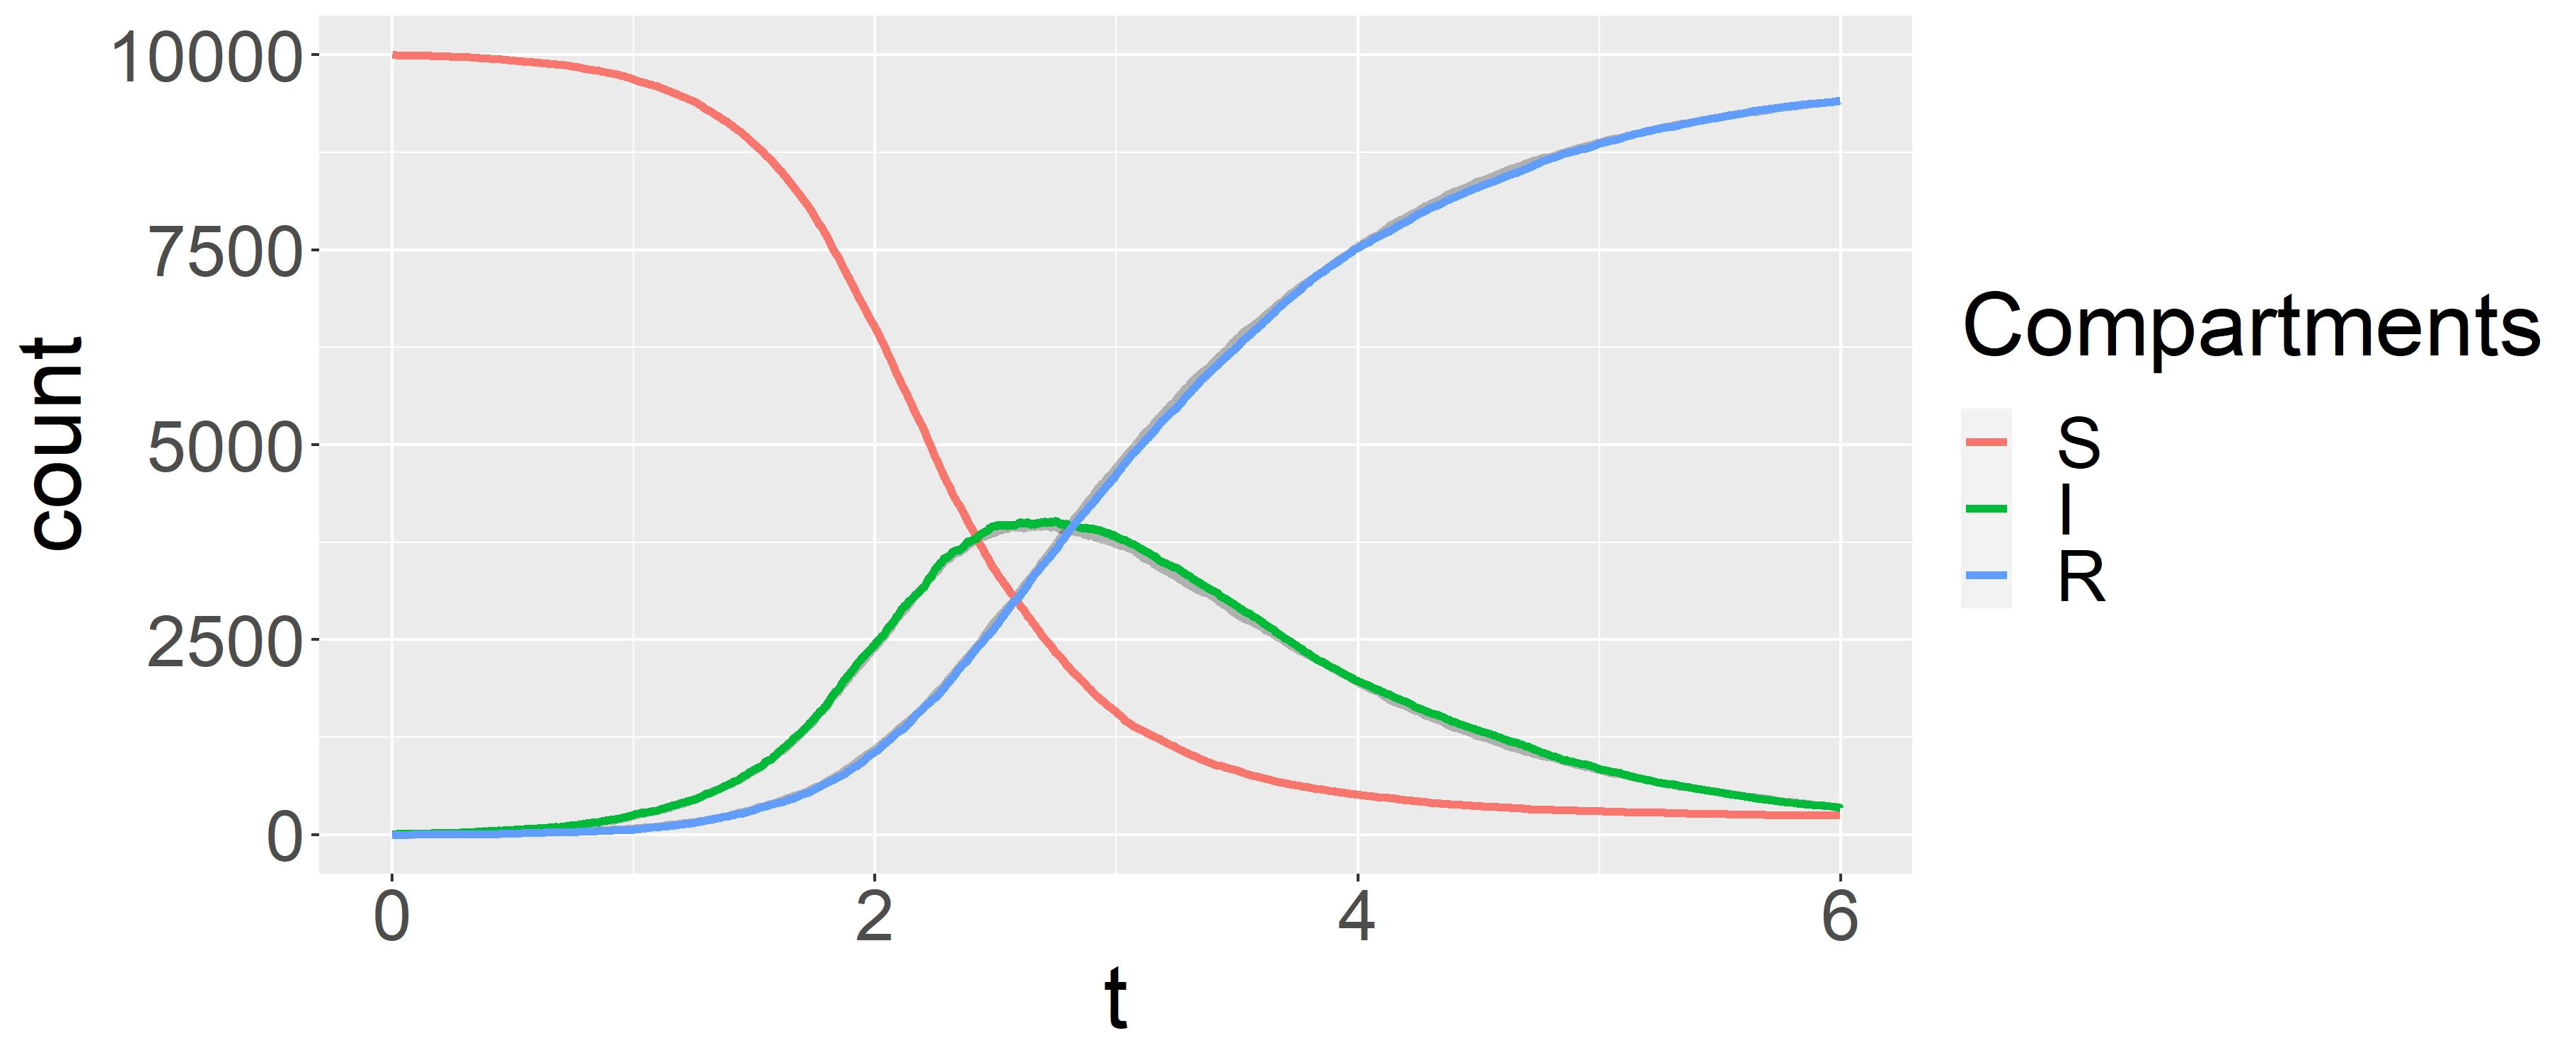
\includegraphics[width=\textwidth]{E2_K1000.jpeg}
			\caption{$K=1000$}
		\end{subfigure}
		\caption{SIR (in color) and PD-SIR process (in grey).}
	\end{figure}
	
\end{frame}


\begin{frame} \frametitle{A Useful Theorem}
	
	\begin{theorem}		
		Consider a LDP with death rate $\mu$ and let $\tau_{1:N} \in (t_l, t_u]$ be the times of the $N$ deaths occurring between times $t_l$ and $t_u$. Then 
		$$\tau_j \,{\buildrel d \over =}\, X_{(j)}, \quad j = 1, \dots, N$$
		where $X_{(j)}$ is the $j^{\text{th}}$ order statistics of $N$ iid random variables following a truncated exponential distribution with rate $\mu$, lower bound $t_l$ and upper bound $t_u$.		
	\end{theorem}
	\vspace{0.5cm}
	$\Rightarrow$ In the PD-SIR process, $z^I_{\mathscr{I}_k}|I_k \sim \TruncExp(\mu_k; t_{k-1}, t_k)$ iid.

\end{frame}


\begin{frame} \frametitle{Simulating the PD-SIR -- pseudo-algorithm}  
	
	\begin{algorithm*}[H]
		\SetAlgoLined
		%	\KwIn{$\theta = (\beta, \lambda), \Y = I_{1:K}$}
		\KwOut{$\Z^\star = \{(z^I_i, z^R_i)\}_i$ compatible with $\Y = I_{1:K}$}
		\For{interval $k = 1, \dots, K$}{
			\vspace{0.2cm}
			Compute the infection rate: \\
			\hspace{0.5cm} $\mu_k \leftarrow \beta I(t_{k-1})$ \\
			\vspace{0.2cm}
			Jointly generate the infection times: \\
			\hspace{0.5cm} $z^I_j \stackrel{iid}{\sim} \TruncExp(\mu_k; t_{k-1}, t_k)$, for $j \in \mathscr{I}_k$ \\
			\vspace{0.2cm}
			Generate the removal times:\\
			\hspace{0.5cm} $z^R_j | z^I_j \stackrel{indep.}{\sim} z^I_j + Exponential(\gamma)$, for $j \in \mathscr{I}_k$
		}
		\caption{Simulating a PD-SIR process conditionally on $\Y$}
	\end{algorithm*}
		
\end{frame}


\begin{frame} \frametitle{A few Remarks on the PD-SIR}  
	
	\begin{itemize}
		\item The DA-MCMC can be initialized with $\theta^{(0)} = \left( \beta^{(0)}, \gamma^{(0)}\right)$ only.
		\item Gibbs-like scheme: $\Z^\star \perp \Z^{(k-1)} | \theta^{(k)}$.
		\begin{itemize}
			\item Uniform ergodicity
		\end{itemize}
		\item Efficient: 
		\begin{itemize}
			\item $\Z^\star$ is compatible with $\Y = I_{1:K}$ by construction.
			\item High MH acceptance rate due to close resemblance between the PD-SIR and SIR processes.			
		\end{itemize}
		\item Fast:
		\begin{itemize}
			\item Only requires uniform RVs (inverse CDF),
			\item Vectorized implementation (rate $\mu_k$ is only updated $K$ times).
		\end{itemize}
	\end{itemize}
\end{frame}

\begin{frame} \frametitle{Uniform Ergodicity}  
	
	A Markov chain is \textit{uniformly ergodic} if for some finite $M$ and positive constant $r<1$, the $n$-step transition kernel $P^n$ satisfies
	$$
	\Vert P^n(x,.)-\pi(.)\Vert_{TV} \le M r^n, \quad \forall x \in \chi
	$$
	
	\begin{itemize}
		\item Uniform ergodicity ensures a CLT (Jones, 2004).
	\end{itemize}
\vfill
	We show that the state space $\chi = \chi_\theta \times \chi_\z$ is a \textit{small set},
	\begin{equation*}
		P(x,.)^m \ge \epsilon \nu(.), \quad \forall x\in \chi
	\end{equation*}
	for some measure $\nu$, positive integer $m$ ($m=1$) and constant $\epsilon > 0$, which holds iff $P$ is uniformly ergodic (Tierney, 1994).
\end{frame}

\begin{frame} \frametitle{Uniform Ergodicity -- Gist of Proof}  


\begin{itemize}
	\item $P = P_{\theta} P_{\z}$ is composite:
	$$\x_1 = (\theta_1, \z_1) \rightarrow (\theta_2, \z_1) \rightarrow (\theta_2, \z_2) = \x_2.$$
	\item Minorize $P_{\theta}$ and $P_{\z}$ separately.
	\begin{itemize}
		\item $P_\theta$: $q_\theta(\theta_2|\z_1)$ is a product of two gammas with bounded parameters.
		\item $P_\z$: $q_\z(\z_2|\theta_2)$ is a product of positive factors (truncated exponentials and tail probabilities).
	\end{itemize}
	\item Interesting result, since the requirement that the whole space be small is typically not satisfied for models with unbounded spaces e.g.\ $\chi_\theta = \R^+\times\R^+$.
\end{itemize}

\end{frame}
	
	


\begin{frame} \frametitle{Simulation Study -- Proof of Concept}  
	\begin{itemize}
		\item $n = 1000$;  $(\beta, \lambda) = (0.0025, 1)$ [$R_0 = 2.5$]
		\item $I_{1:10} = (13, 31,  55, 71, 103, 111, 135, 103, 74, 42)$
		\item$(\beta_0, \gamma_0) = (\beta/10, \gamma/10)$ (low density region)
		\item Stationarity is reached within $1500$ iterations
		\item 1e6 iterations take $<30$ minutes on a laptop.
	\end{itemize} 
	
	\begin{figure}
		\centering
		\begin{subfigure}[b]{0.32\textwidth}
			\centering
			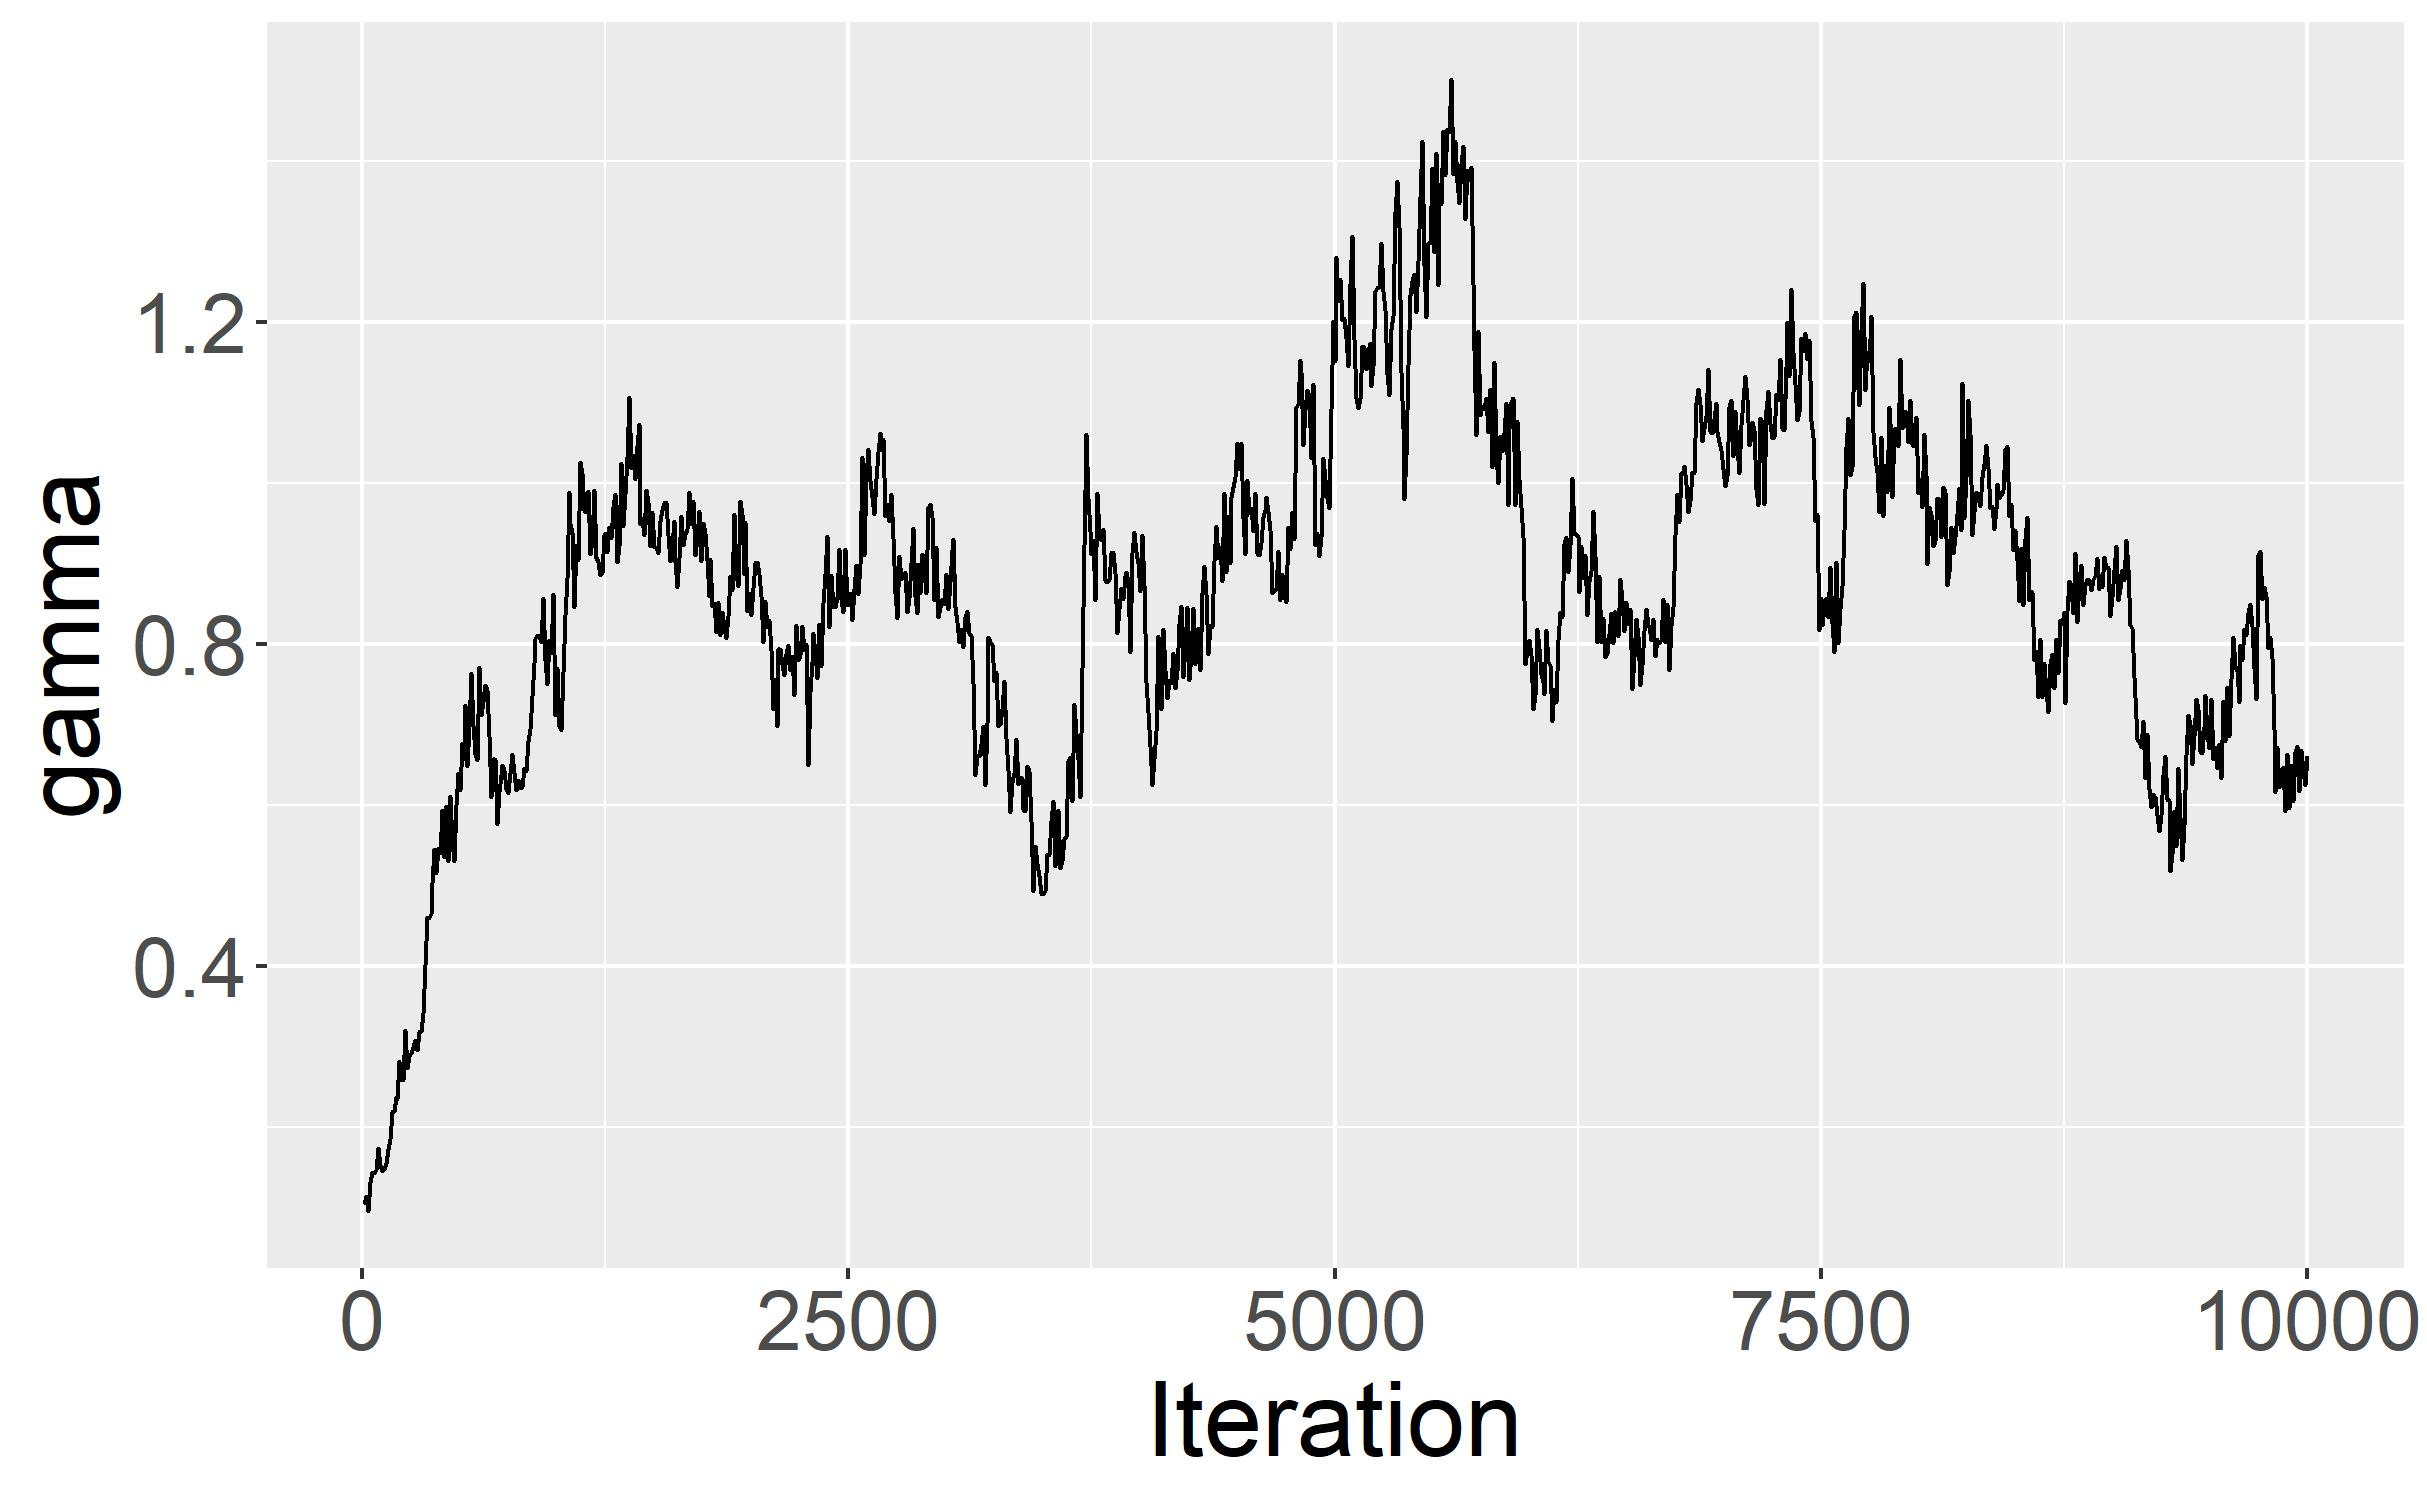
\includegraphics[width=\textwidth]{E1_short_no_burn_gamma_tp}
			\caption{Transient phase}
			\label{fig:E1_short_no_burn_gamma_tp}
		\end{subfigure}
		\hfill
		\begin{subfigure}[b]{0.32\textwidth}
			\centering
			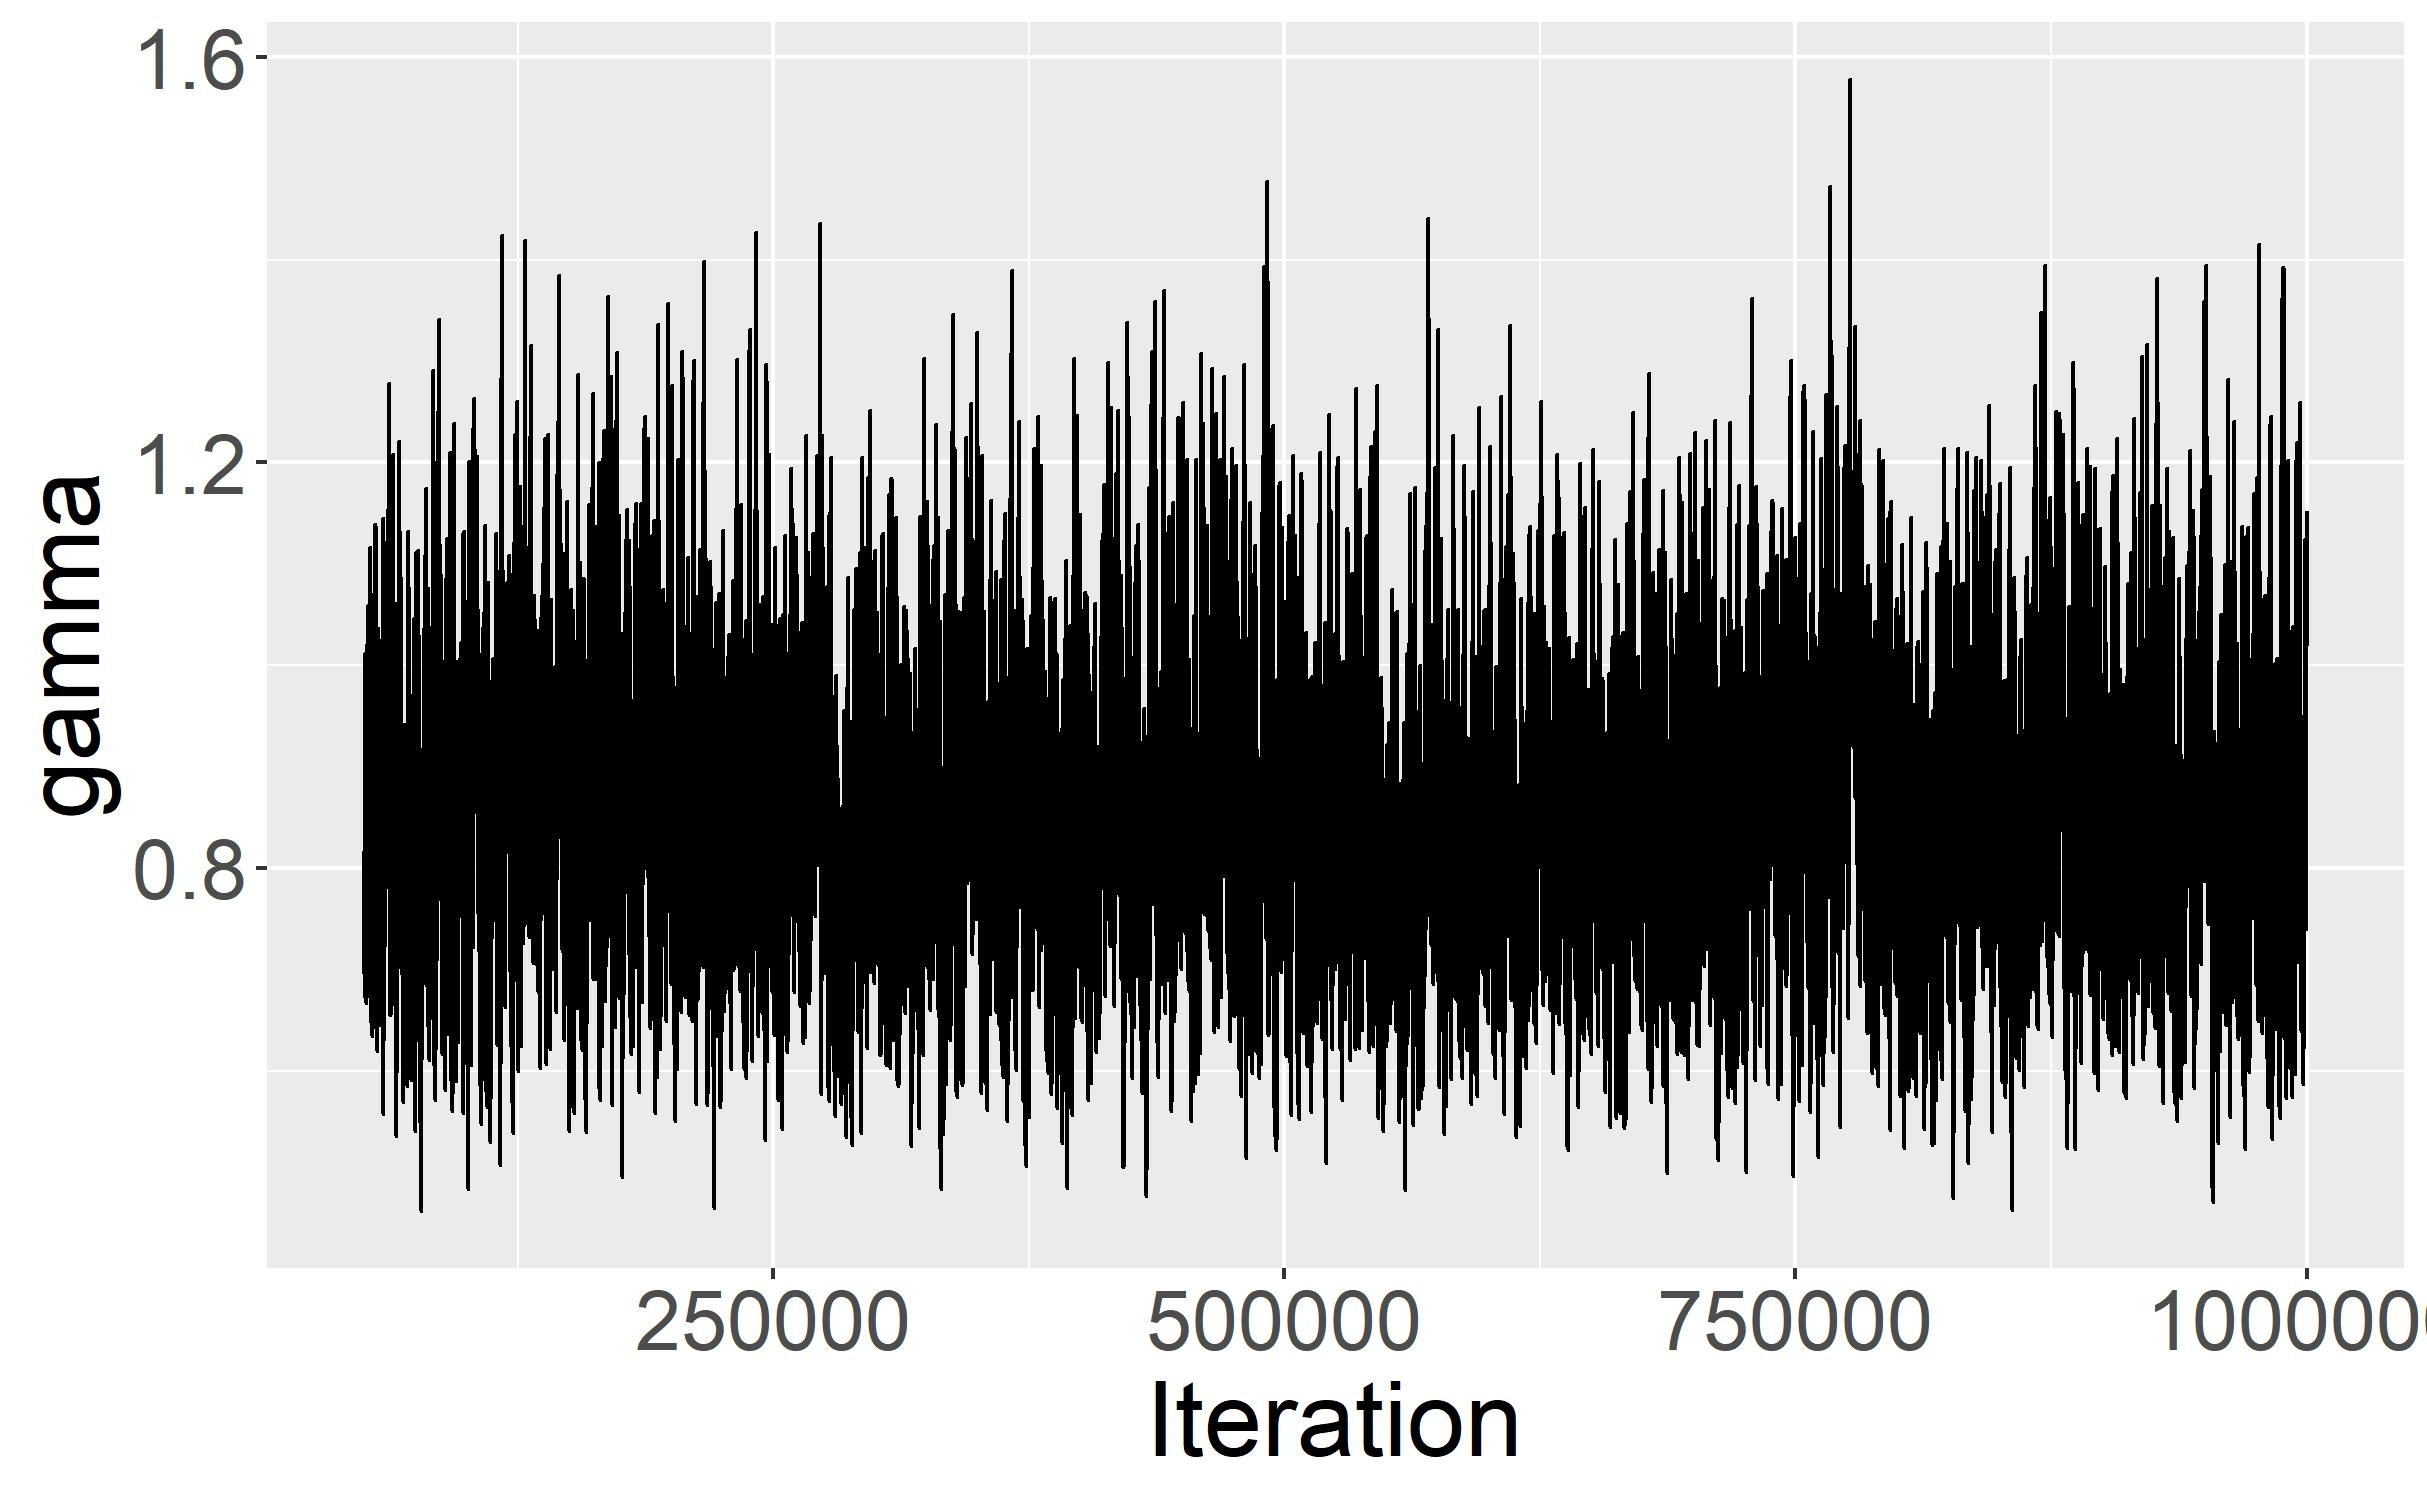
\includegraphics[width=\textwidth]{E1_burn_gamma_tp}
			\caption{Recurrent phase}
			\label{fig:E1_burn_gamma_tp}
		\end{subfigure}
		\hfill
		\begin{subfigure}[b]{0.32\textwidth}
			\centering
			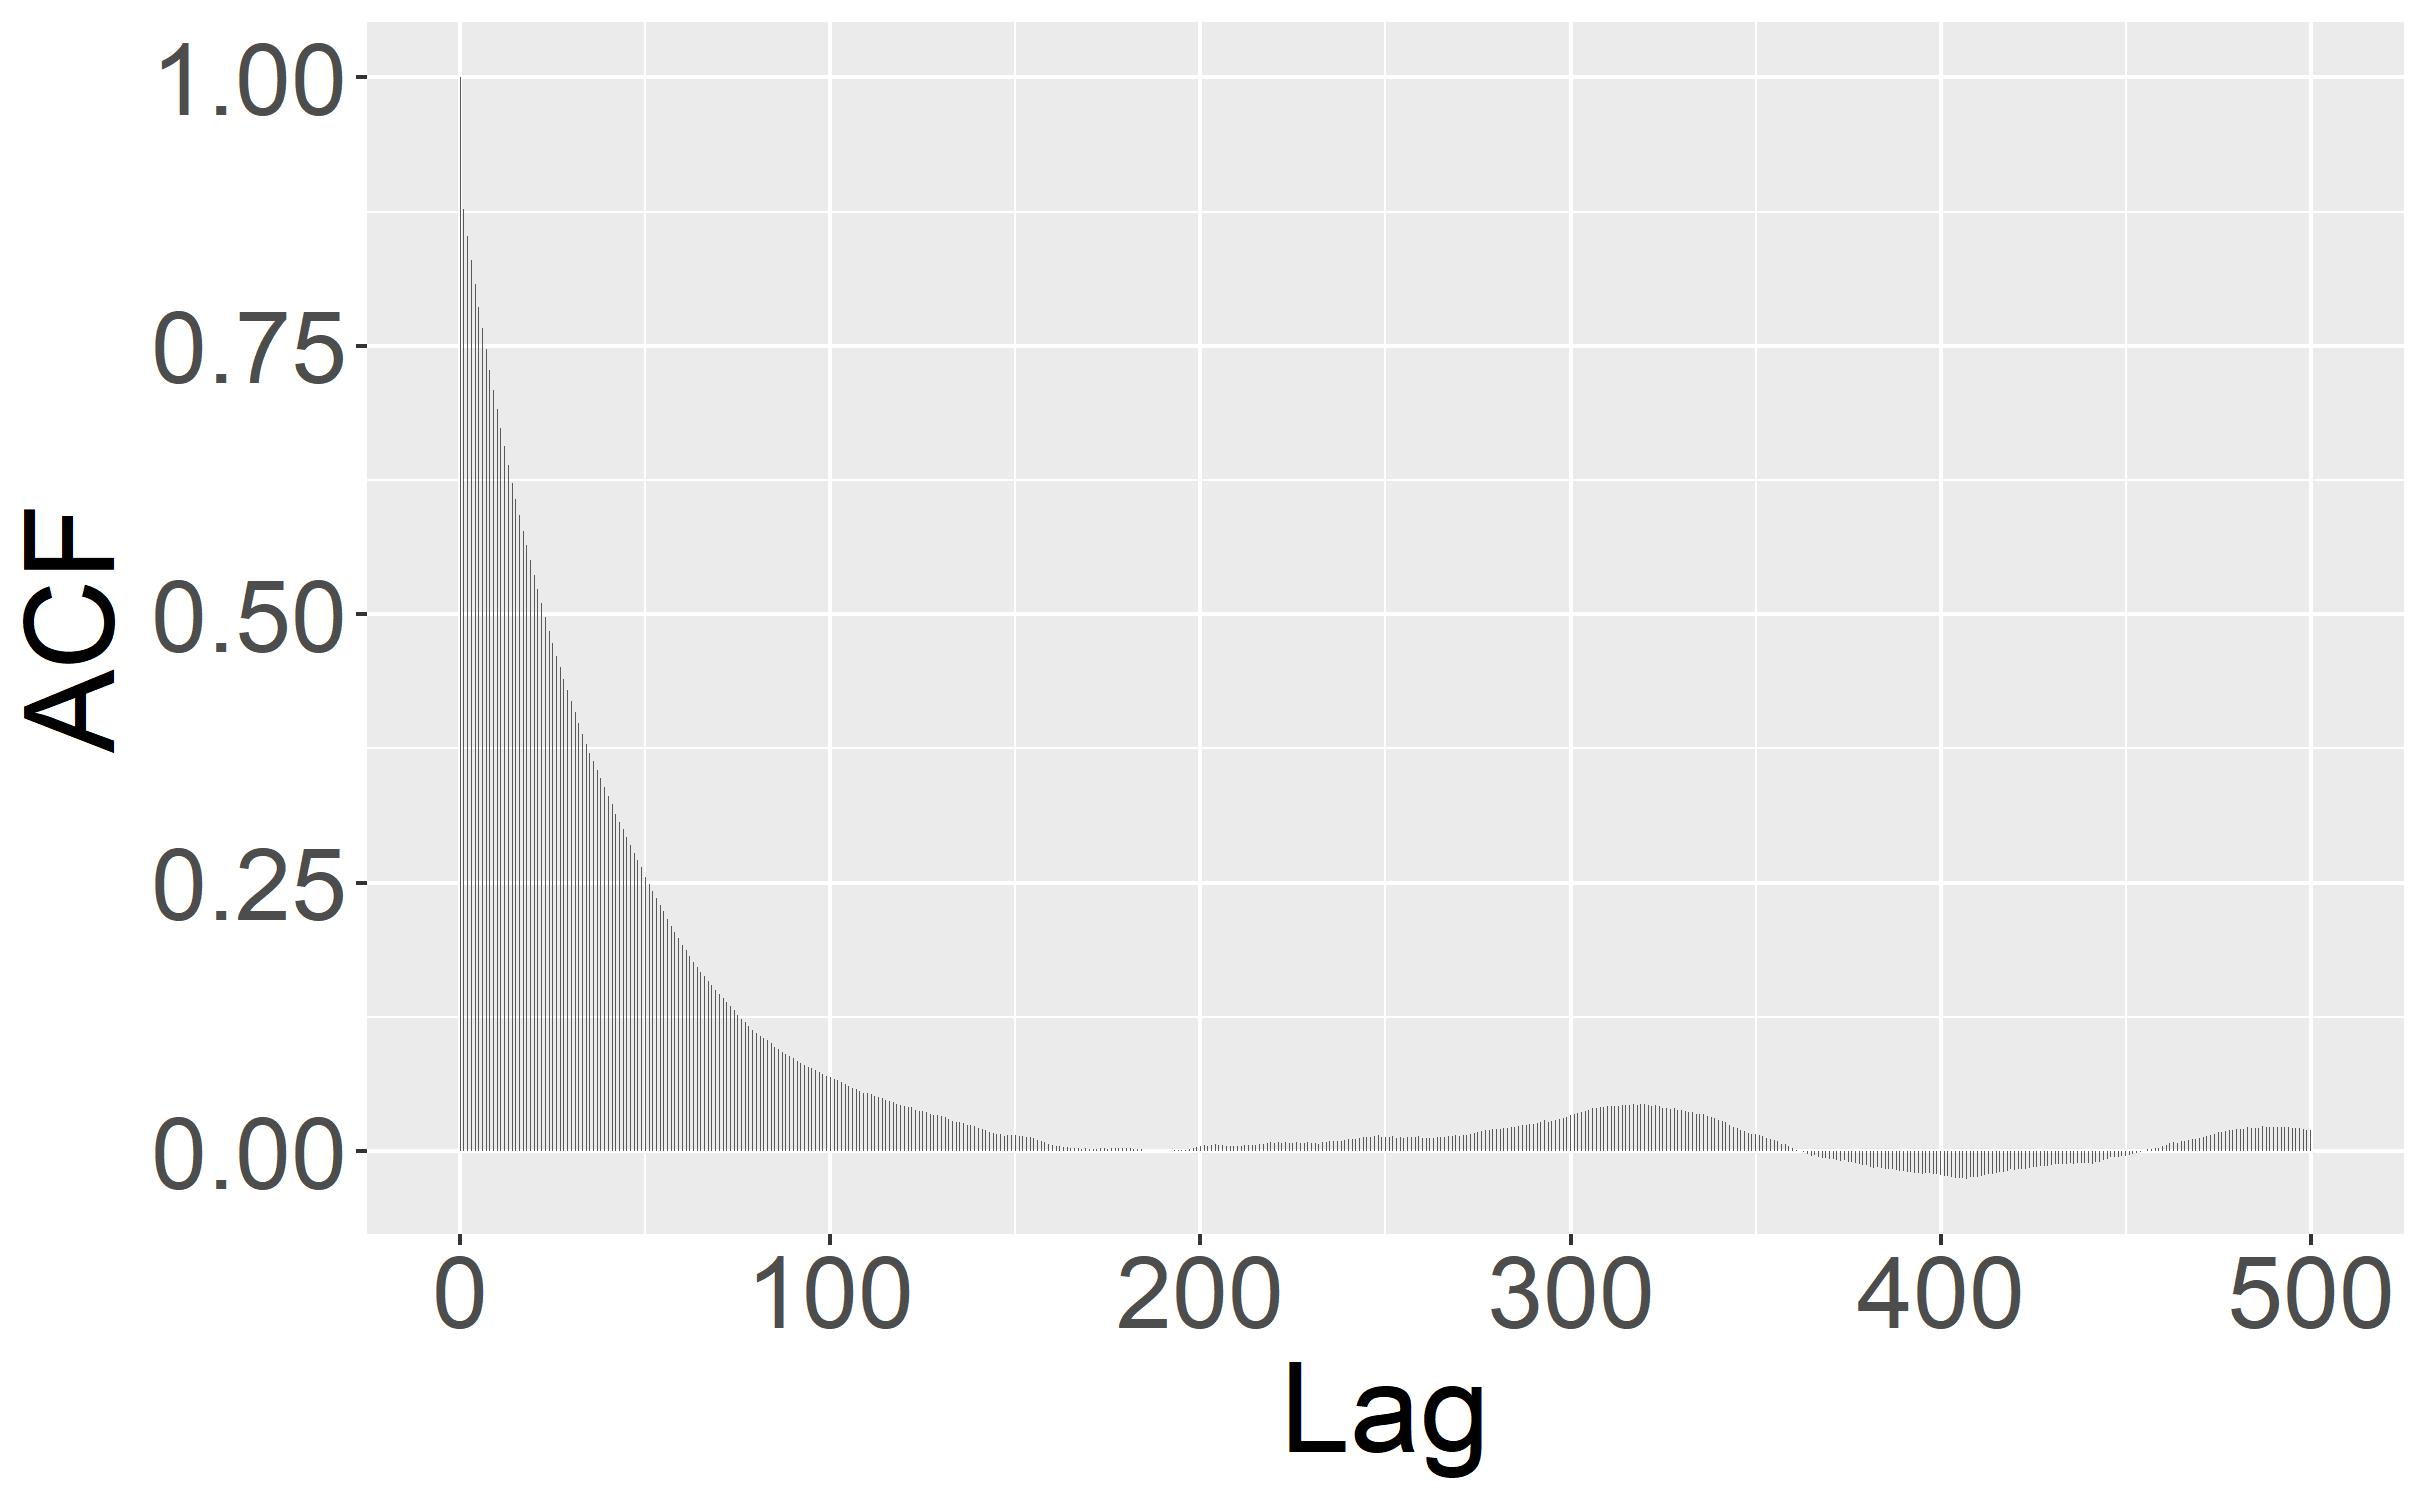
\includegraphics[width=\textwidth]{E6_burn_beta_acf_joint}
			\caption{ACF}
			\label{fig:E1_burn_gamma_acf}
		\end{subfigure}
		\caption{Performance of our DA-MCMC in a medium-sized population.}
		\label{fig:E1}
	\end{figure}
	
\end{frame}


\begin{frame} \frametitle{Simulation Study -- Coverage}  
	\begin{itemize}
		\item Repeat previous experiment 2000 times.
		\item Coverage of $90\%$ credible intervals.
		\item Weakly informative priors: $\beta \sim Ga(0.001,1), R_0 \sim IG(2, 2)$.
	\end{itemize} 
	
	\begin{table}
		\centering
		\begin{tabular}{ C{2cm}| *{3}{C{2.2cm}}}
			%\hline
			Parameter & Observed coverage rate & Average of the posterior means & SD of the posterior means \\ 
			\hline
			$\beta$ (0.0025) & 0.895 & 0.0025 & 0.000255 \\ 
			$\gamma$ (1) & 0.902 & 1.00 & 0.142 \\ 
			$R_0$ (2.5) & 0.910 & 2.54 & 0.194 \\
			\hline
		\end{tabular}
	\end{table}
\end{frame}


\begin{frame} \frametitle{Simulation Study --  Tuning Parameter $\rho$}  
	\begin{itemize}
		\item For large $n$, the MH acceptance rate can be too low.
		\item To improve mixing, only update the trajectories of $\lceil\rho n\rceil$ randomly chosen individuals ($0<\rho\le1$) per iteration.
		\item $n\in(250, 500, 1000)$, $\rho \in (0.02, 0.05, 0.1, 0.25, 0.5, 0.75, 1)$.
	\end{itemize} 
	
\begin{figure}
	\centering
	\begin{subfigure}[b]{0.32\textwidth}
		\centering
		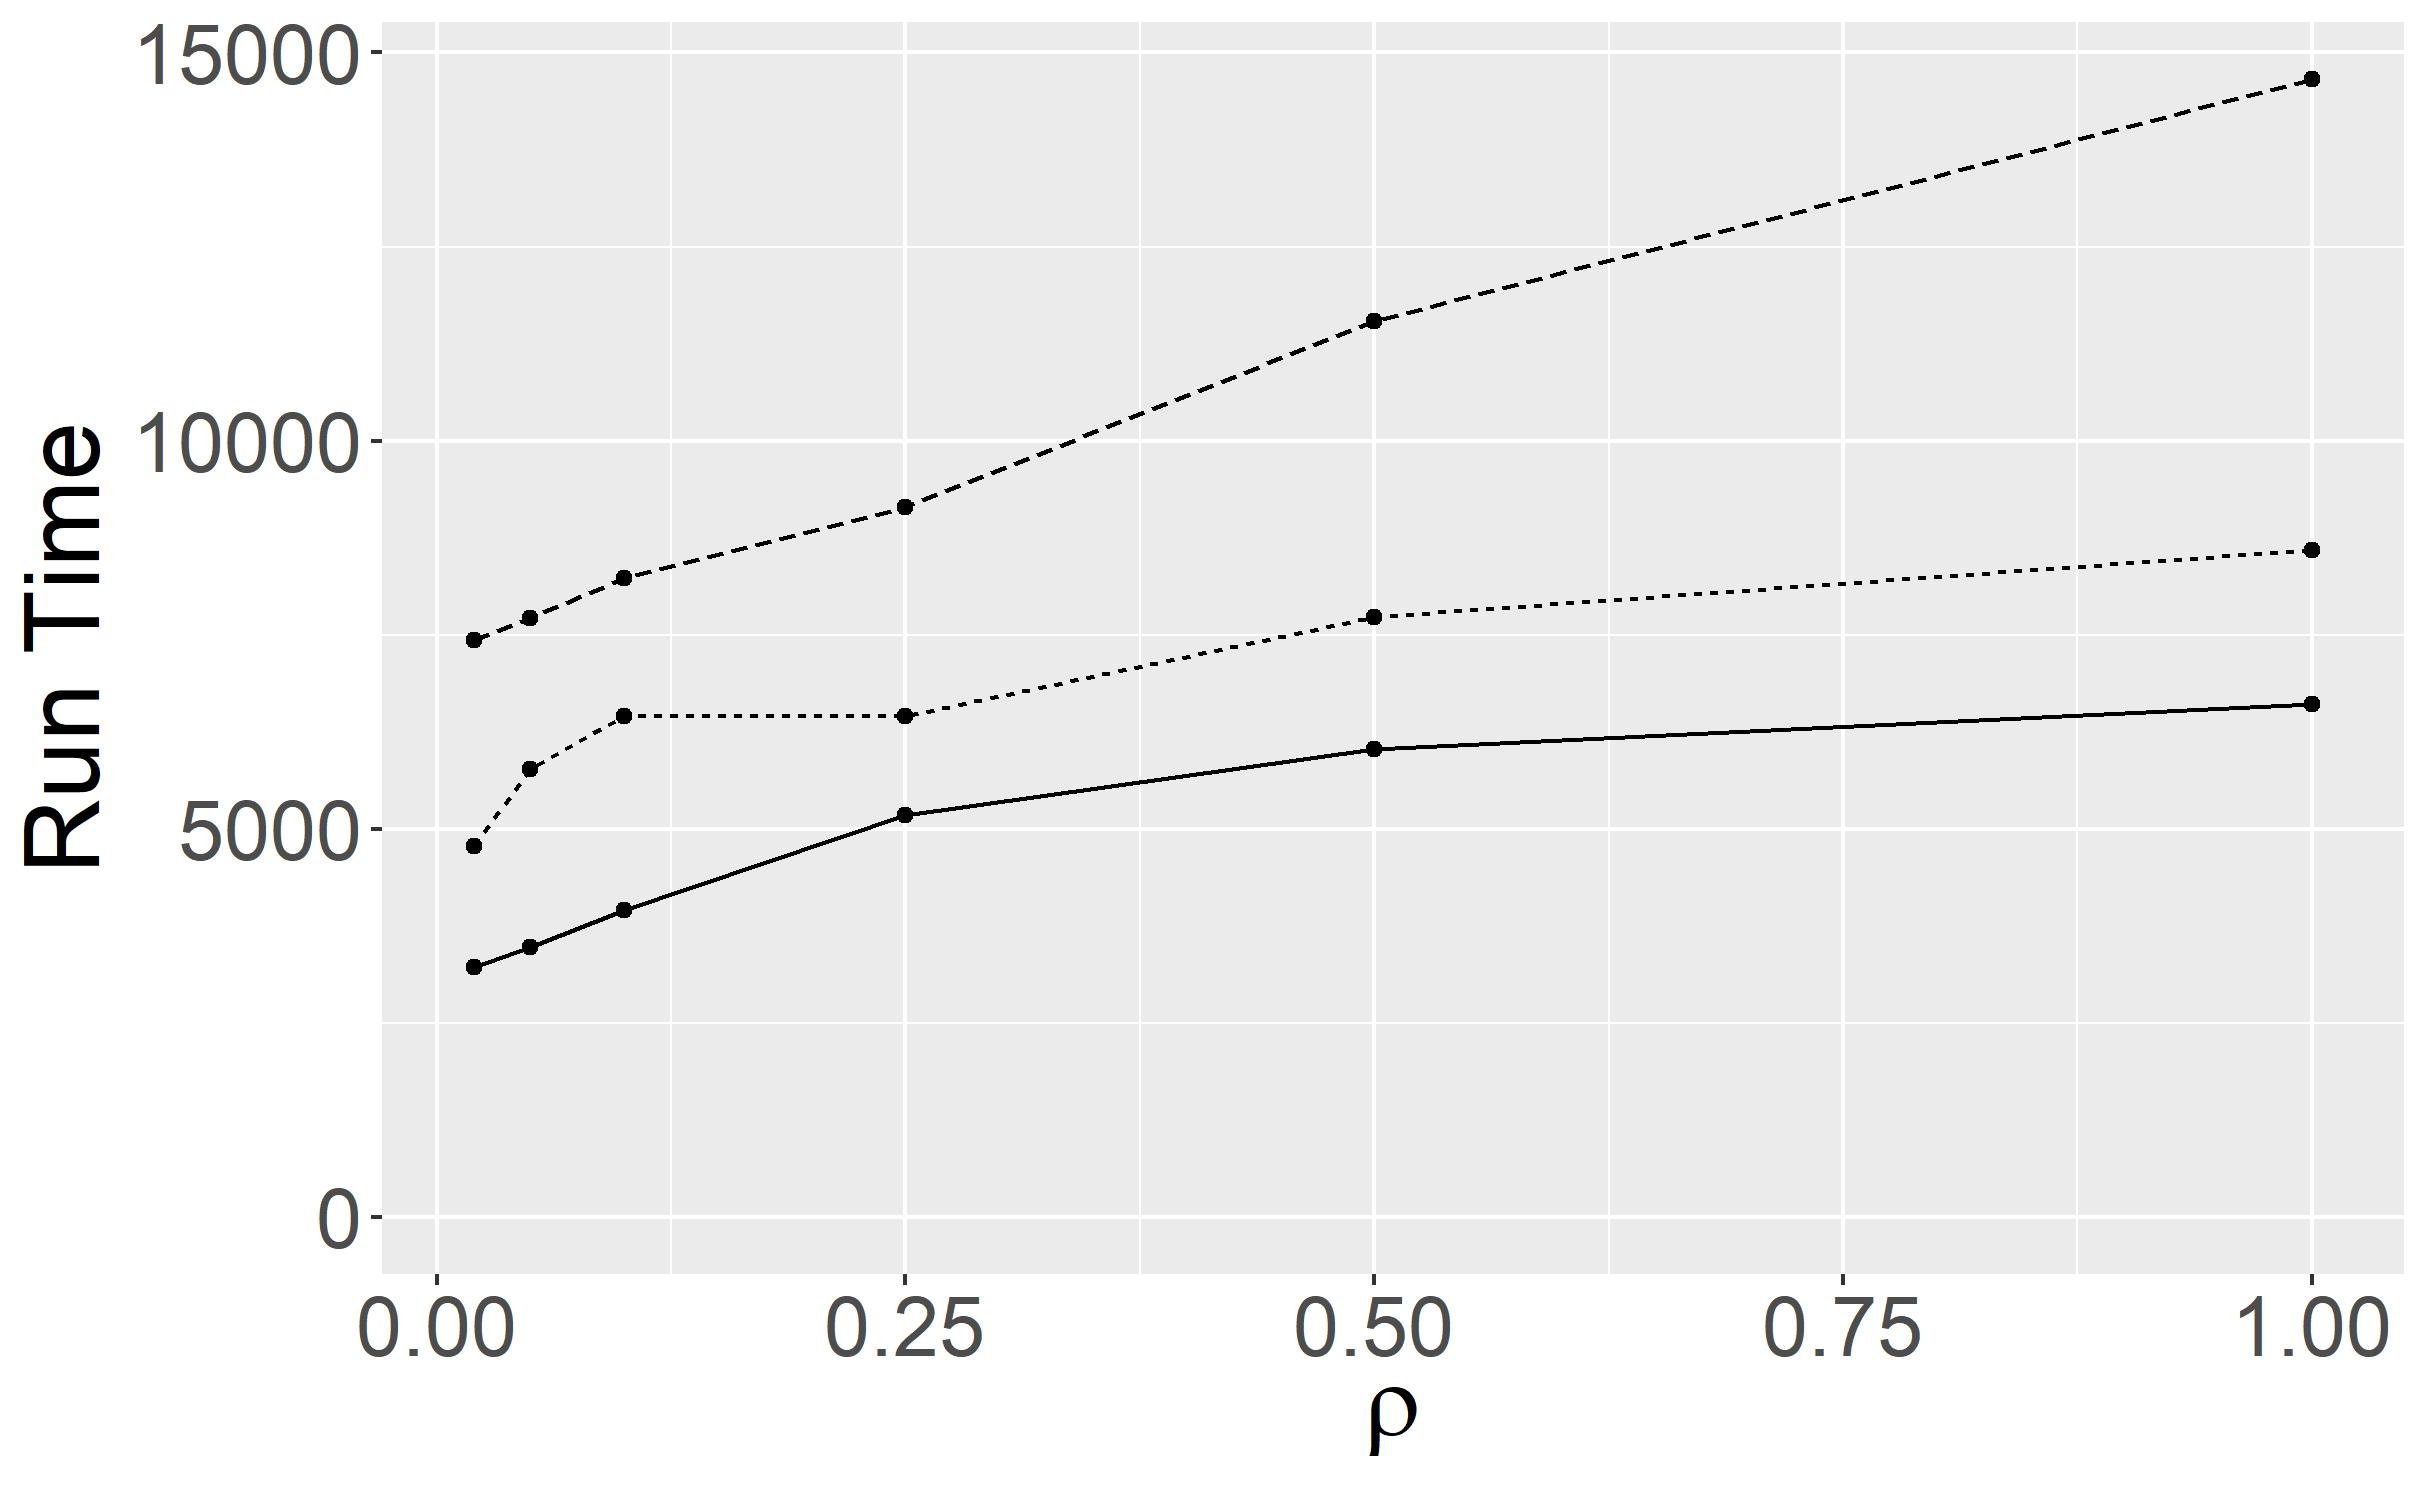
\includegraphics[width=\textwidth]{E3_runtime}
		\caption{Run time in seconds}
		\label{fig:E3_runtime}
	\end{subfigure}
	\hfill
	\begin{subfigure}[b]{0.32\textwidth}
		\centering
		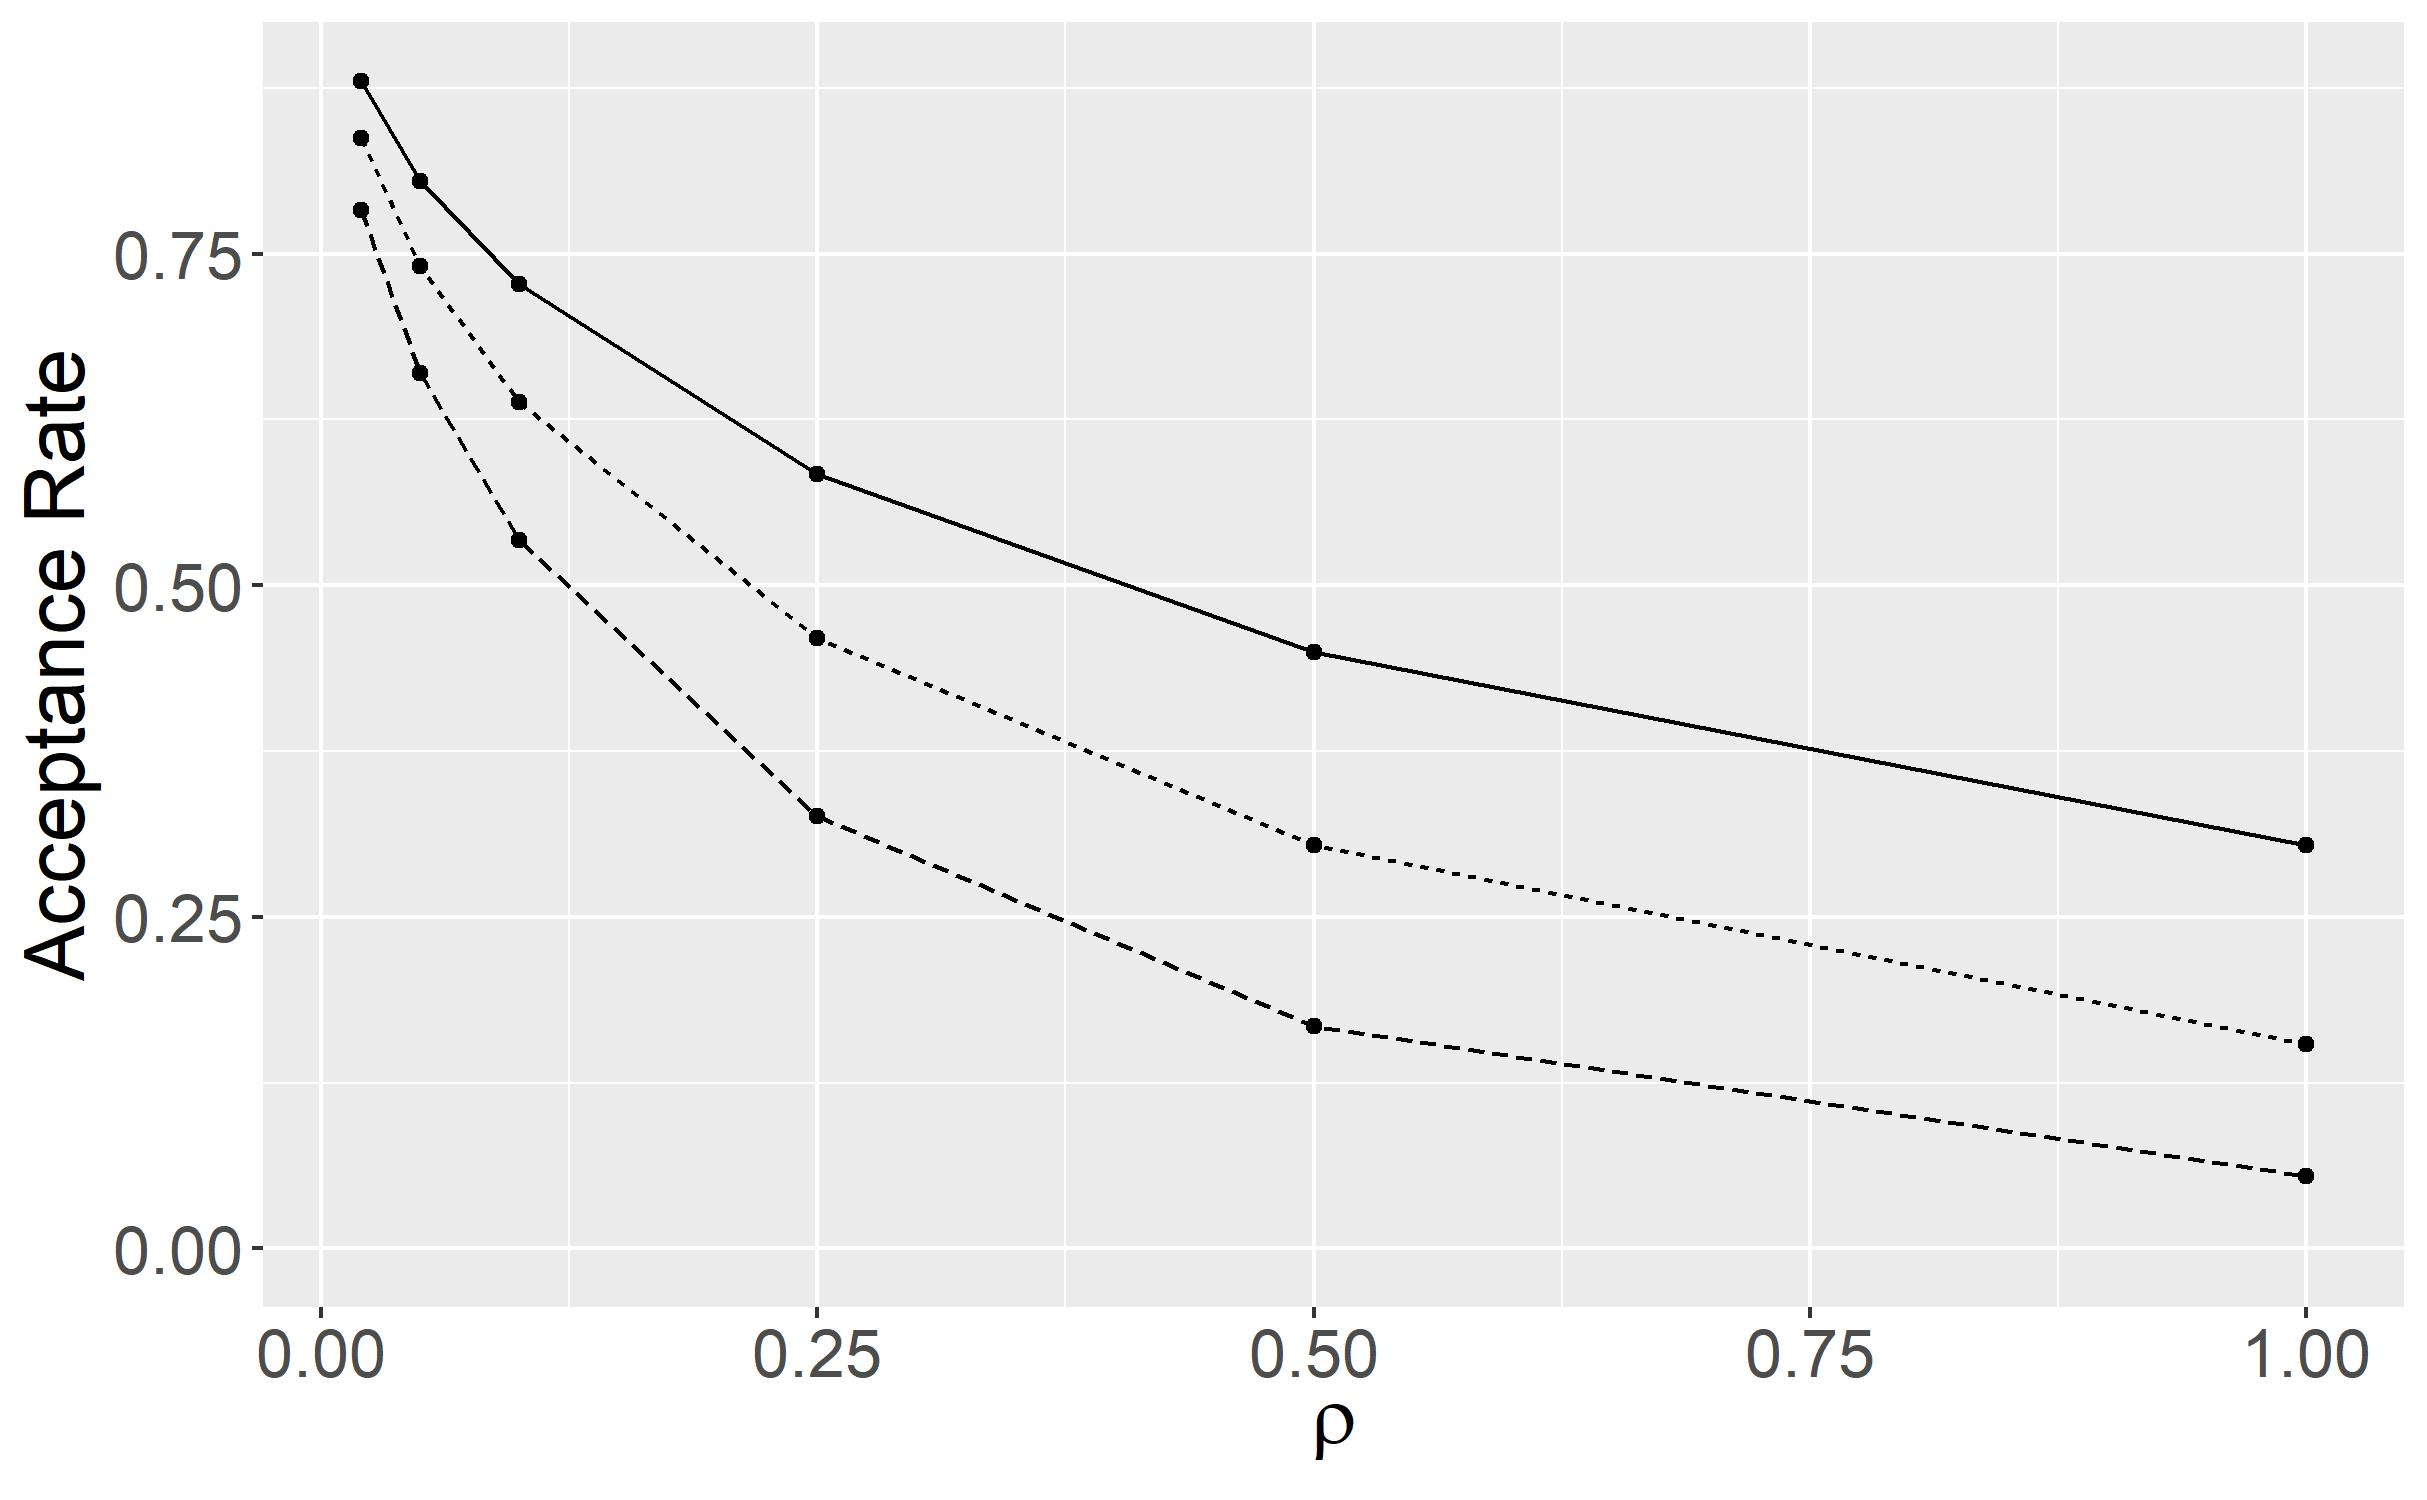
\includegraphics[width=\textwidth]{E3_accept}
		\caption{Acceptance rate}
		\label{fig:E3_accept}
	\end{subfigure}
	\hfill
	\begin{subfigure}[b]{0.32\textwidth}
		\centering
		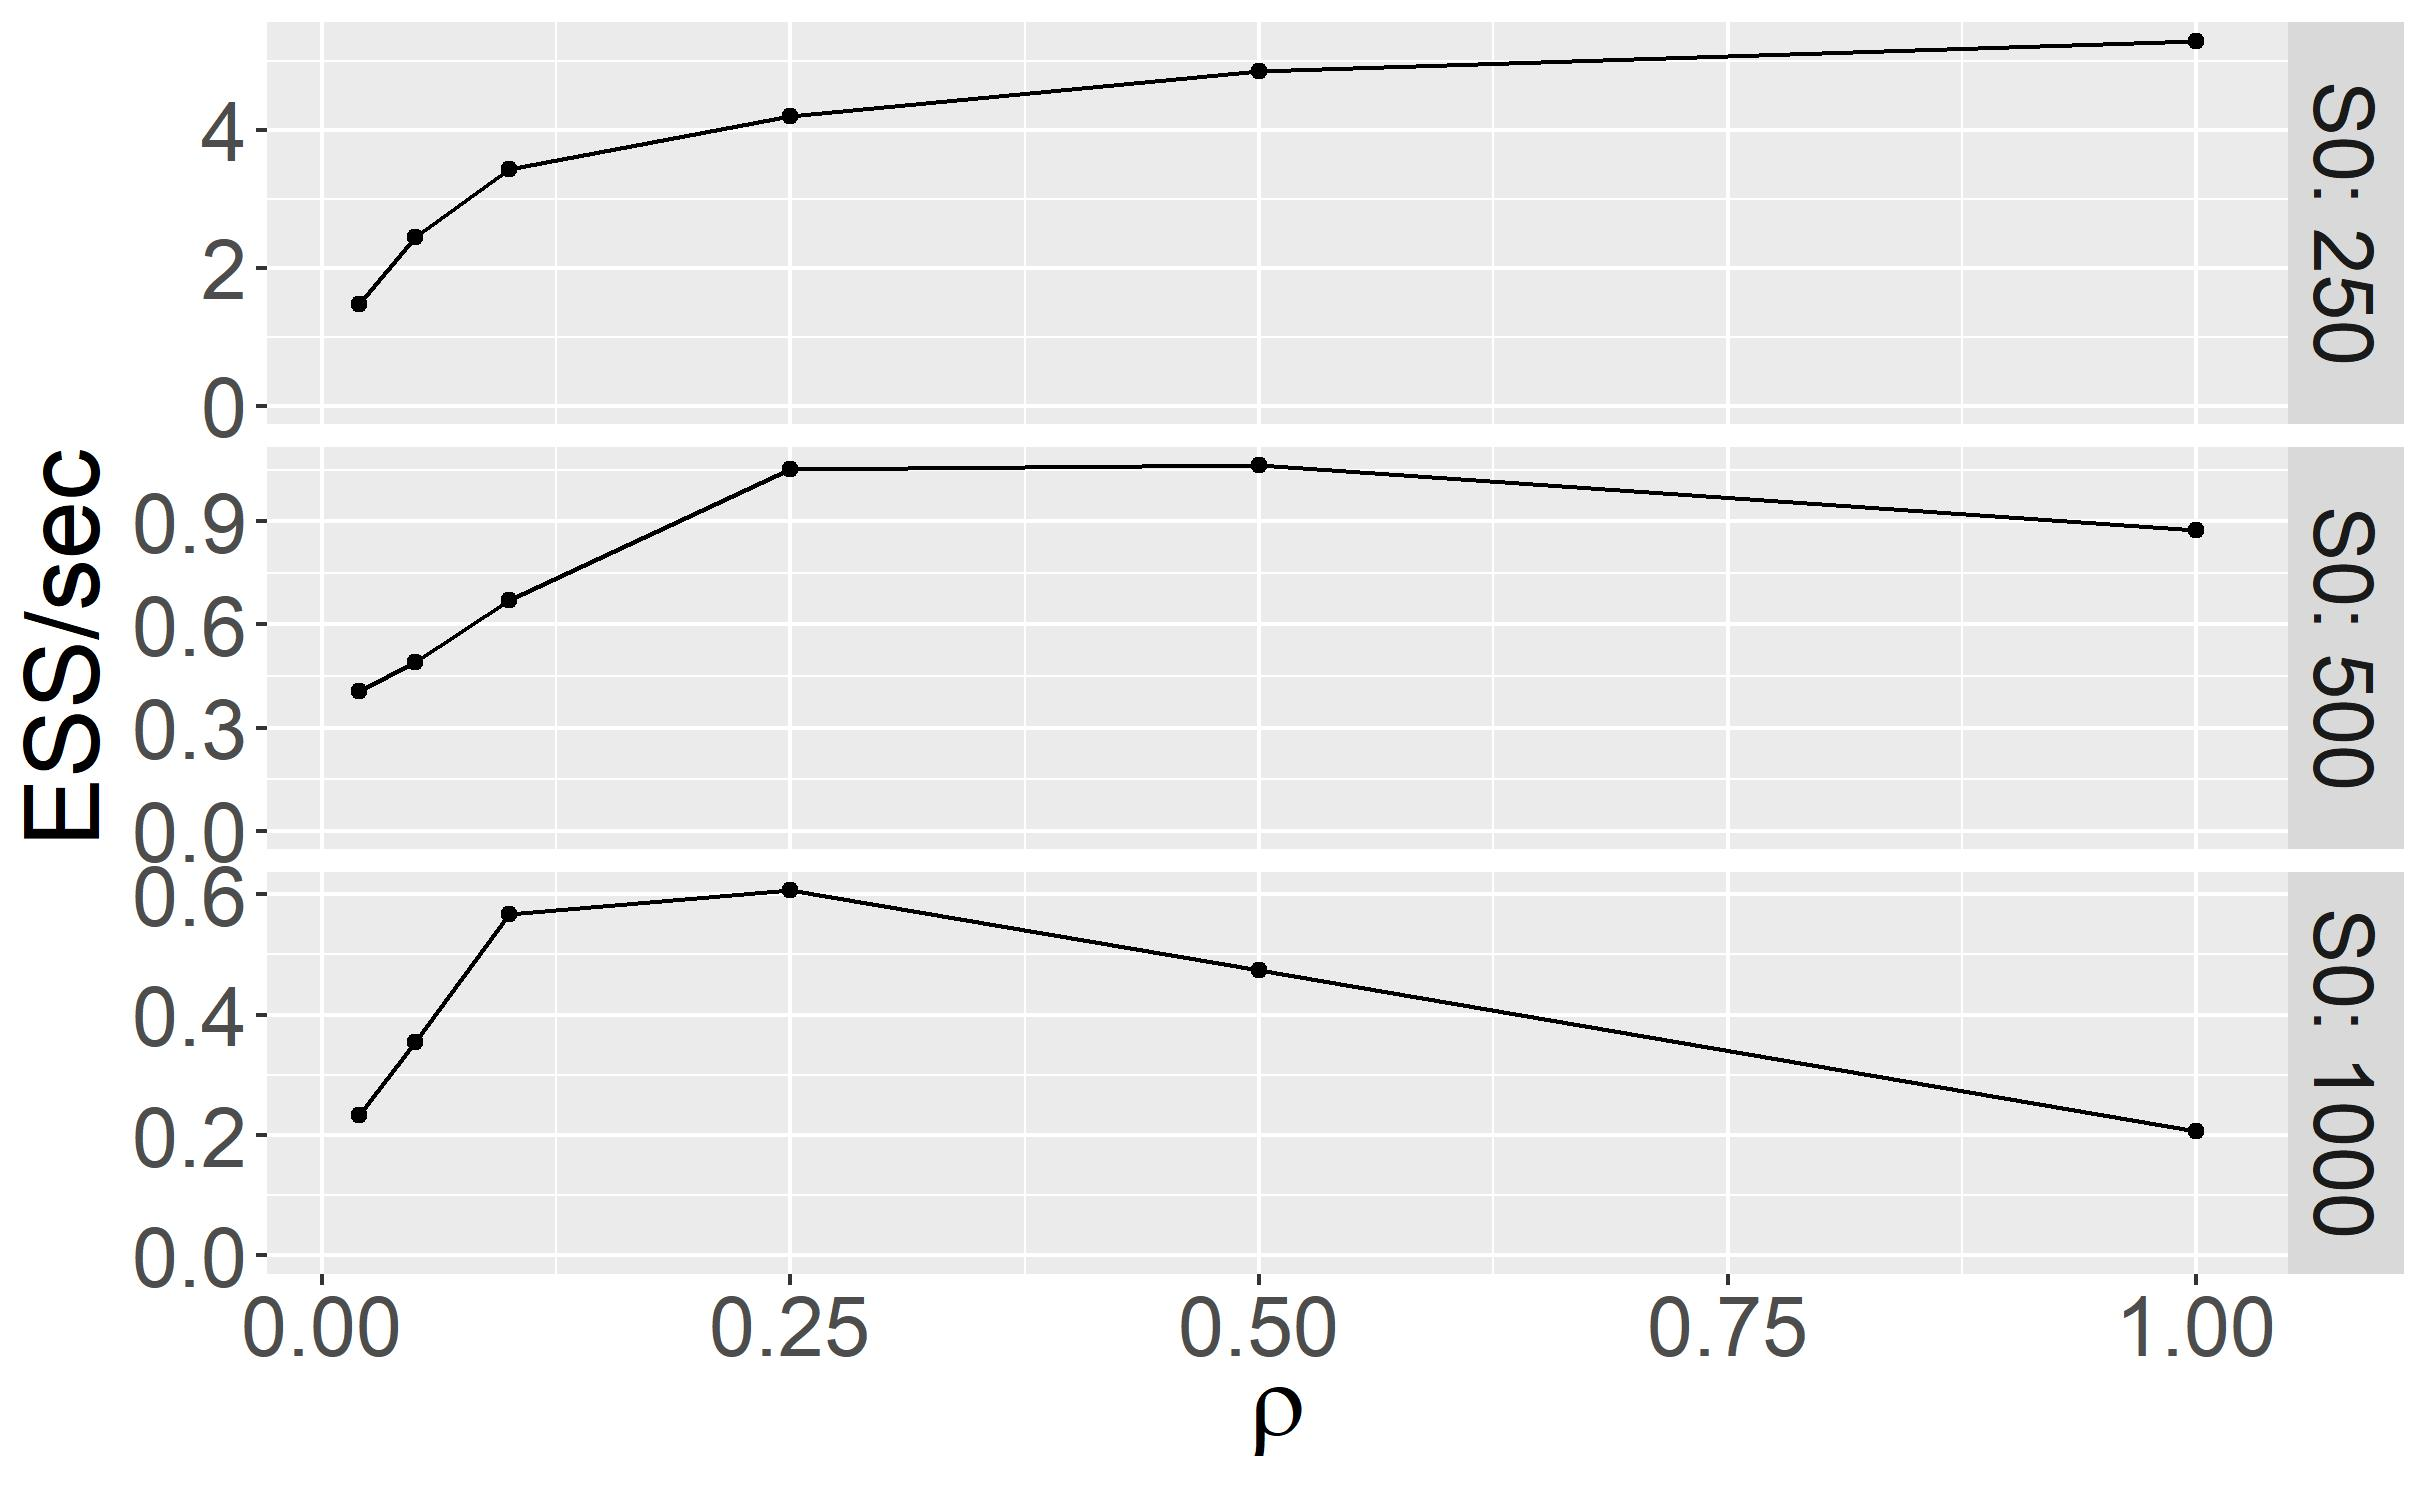
\includegraphics[width=\textwidth]{E3_facet_ESSsecR0}
		\caption{ESS/sec for $R_0$
			%Acceptance rate of the proposed latent spaces in the Metropolis-Hastings step of the MCMC algorithm across different population sizes and values for $\rho$.
		}
		\label{fig:E3_facet_ESSsecR0}
	\end{subfigure}
	\caption{Impact of $\rho$ on the performance of the DA-MCMC in a population of size $250$ (solid), $500$ (dotted) and $1000$ (dashed).}
	\label{fig:E3}
\end{figure}
	
\end{frame}


\begin{frame} \frametitle{Simulation Study --  Comparison with SSU DA-MCMC}  
	
	\begin{figure}
		\centering
		\begin{subfigure}[b]{0.49\textwidth}
			\centering
			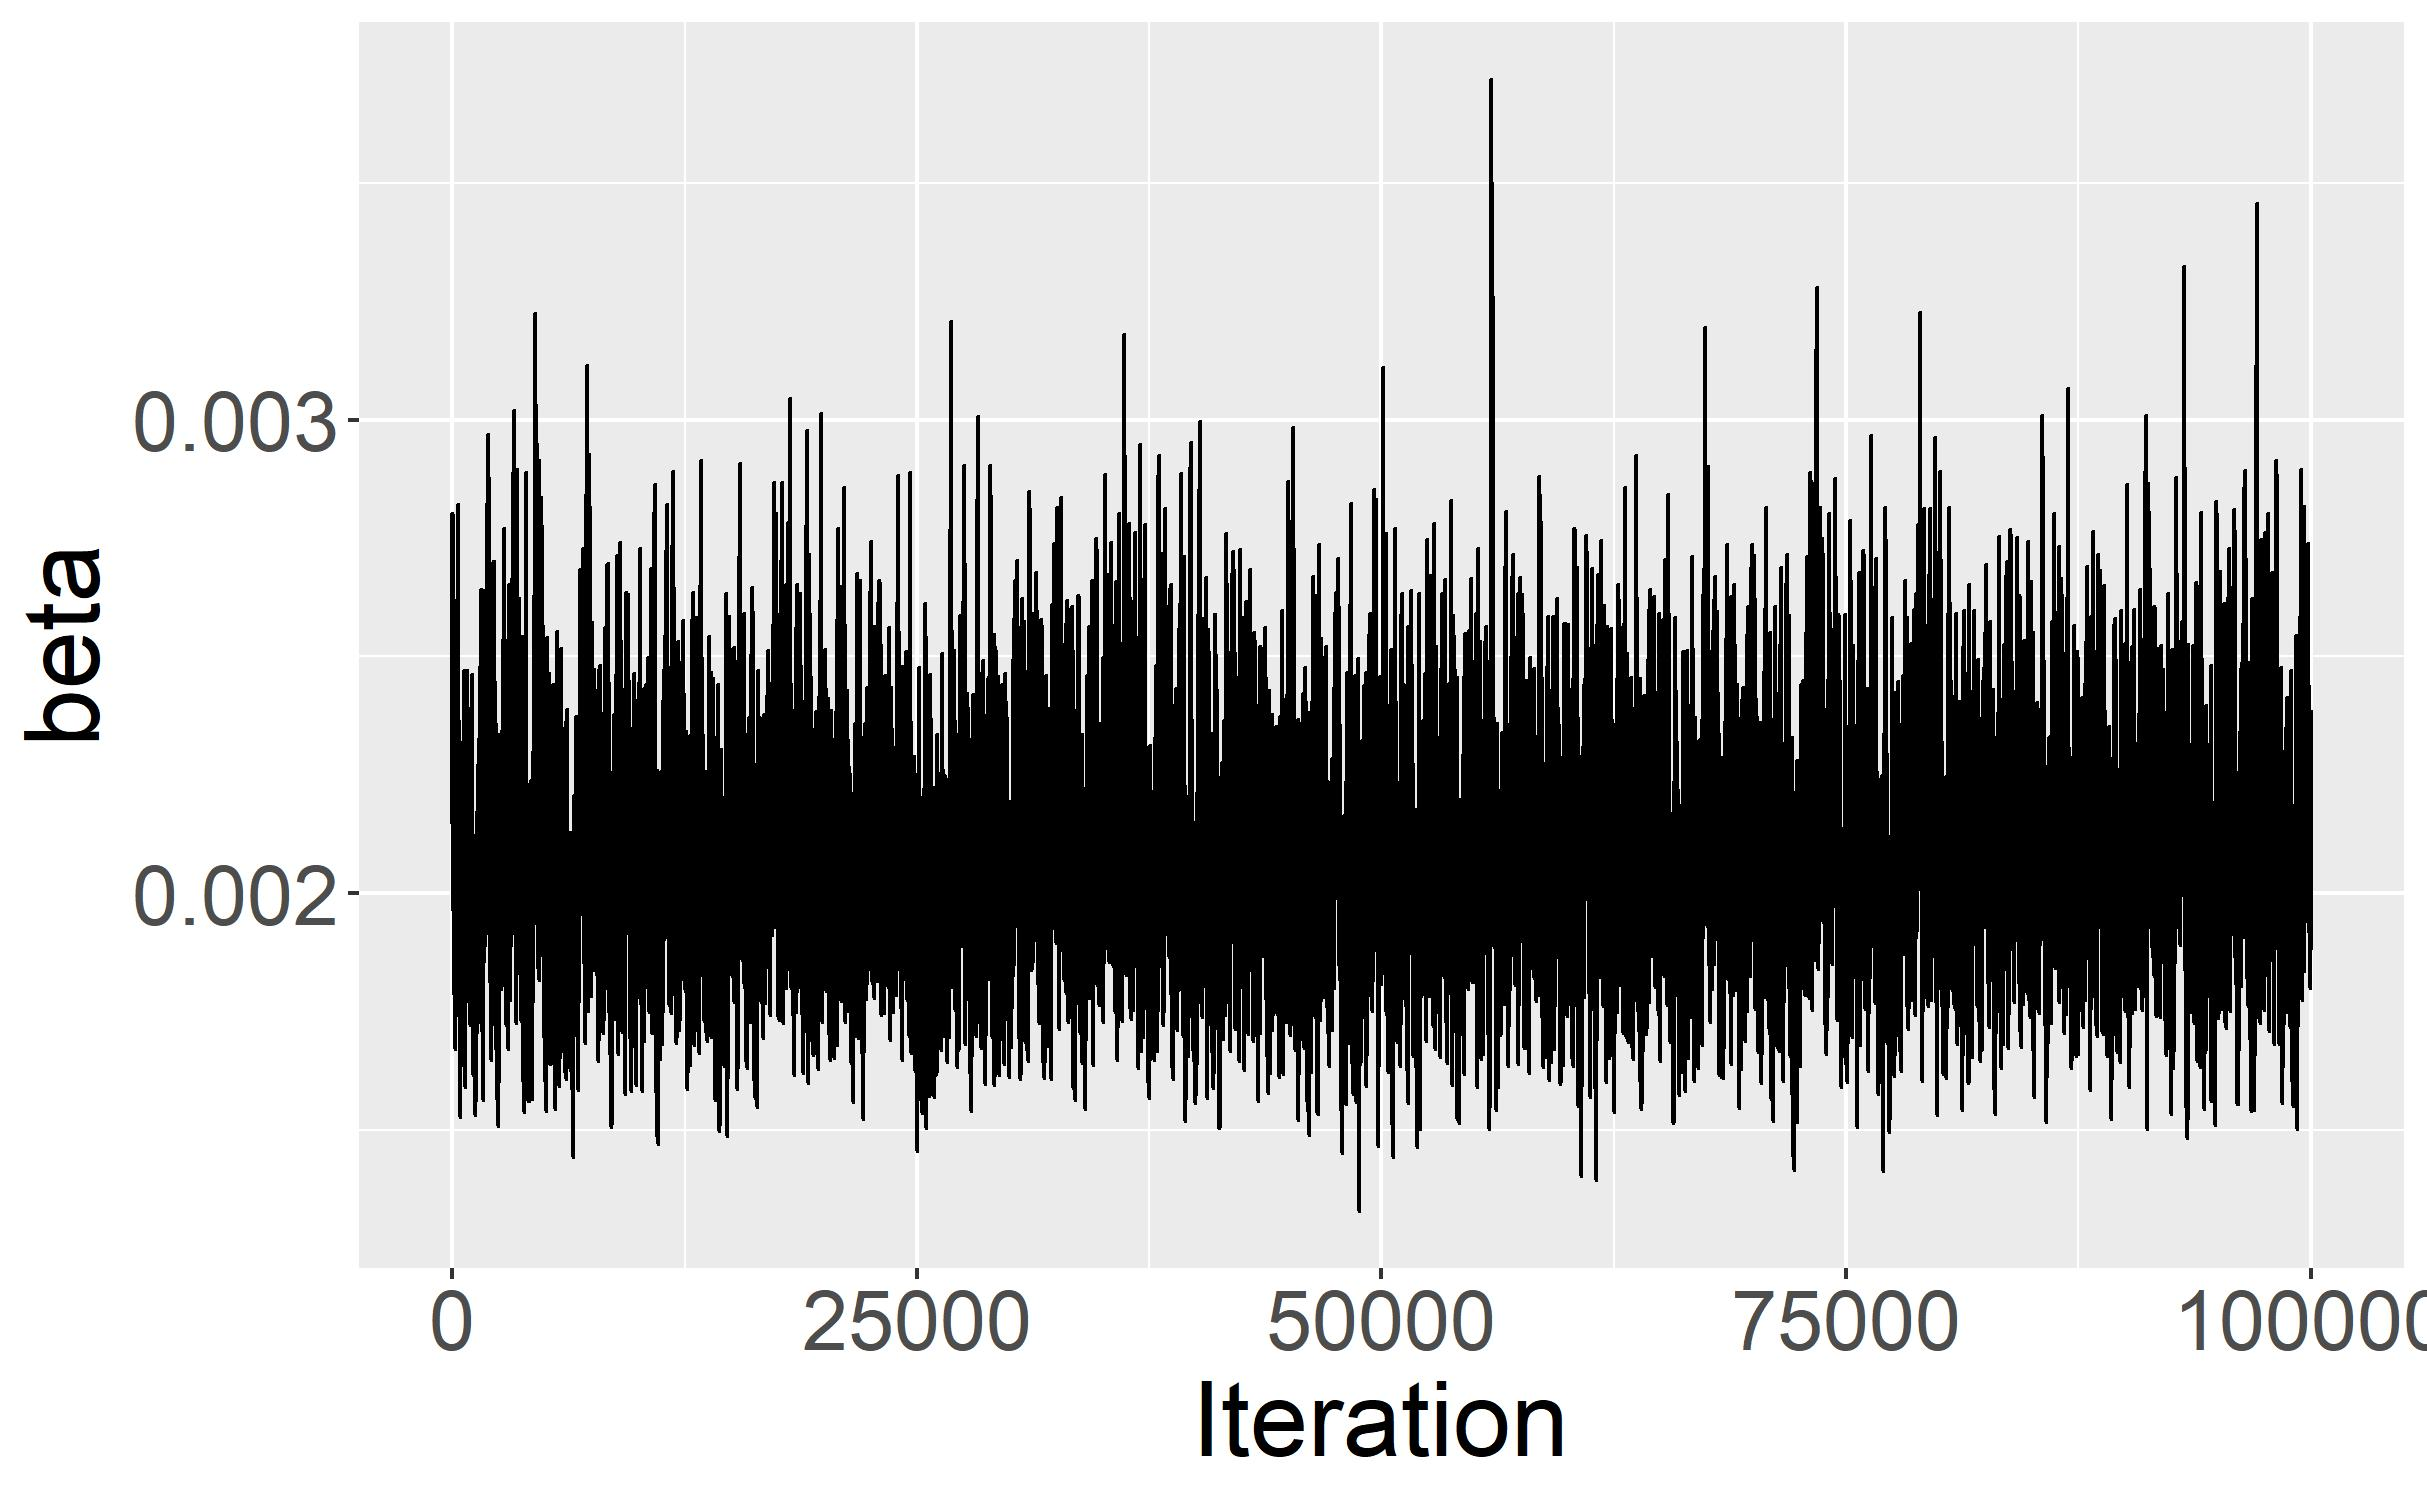
\includegraphics[width=0.48\textwidth]{E6_no_burn_beta_tp_joint.jpg}
			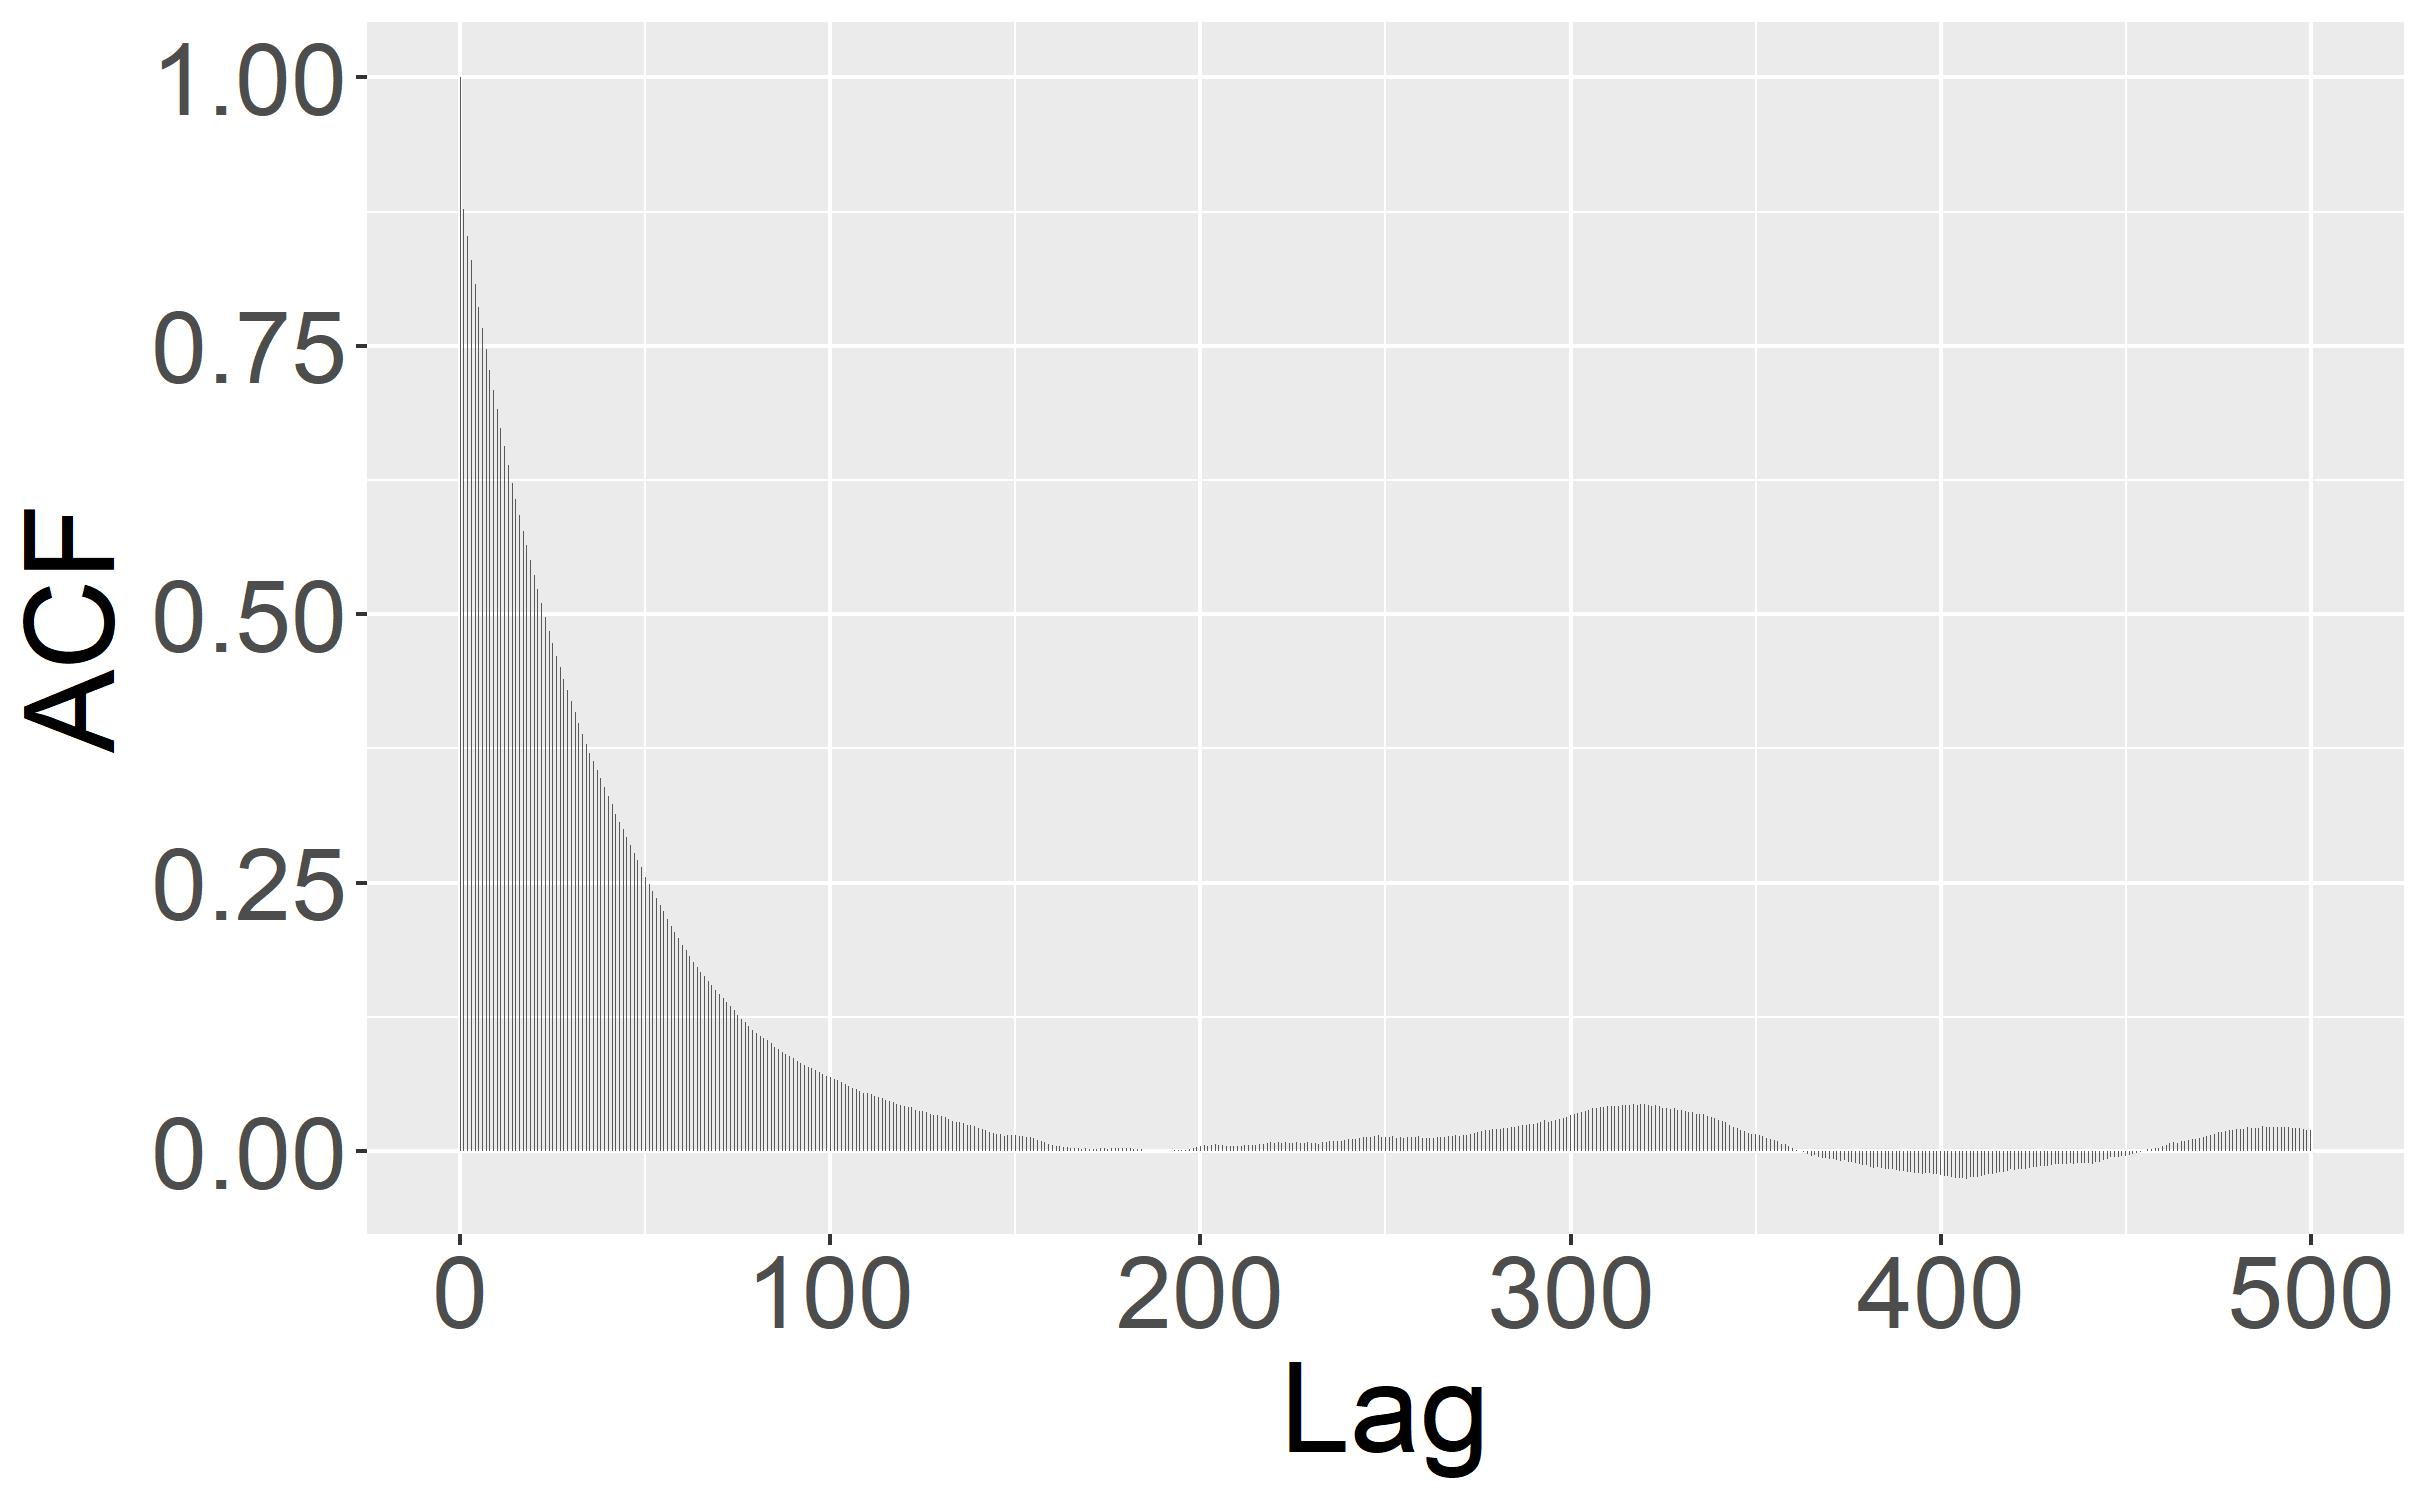
\includegraphics[width=0.48\textwidth]{E6_burn_beta_acf_joint.jpg}
			\caption{DA-MCMC}
			\label{fig:E6_no_burn_beta_tp_joint}
		\end{subfigure}
		\hfill
		\begin{subfigure}[b]{0.49\textwidth}
			\centering
			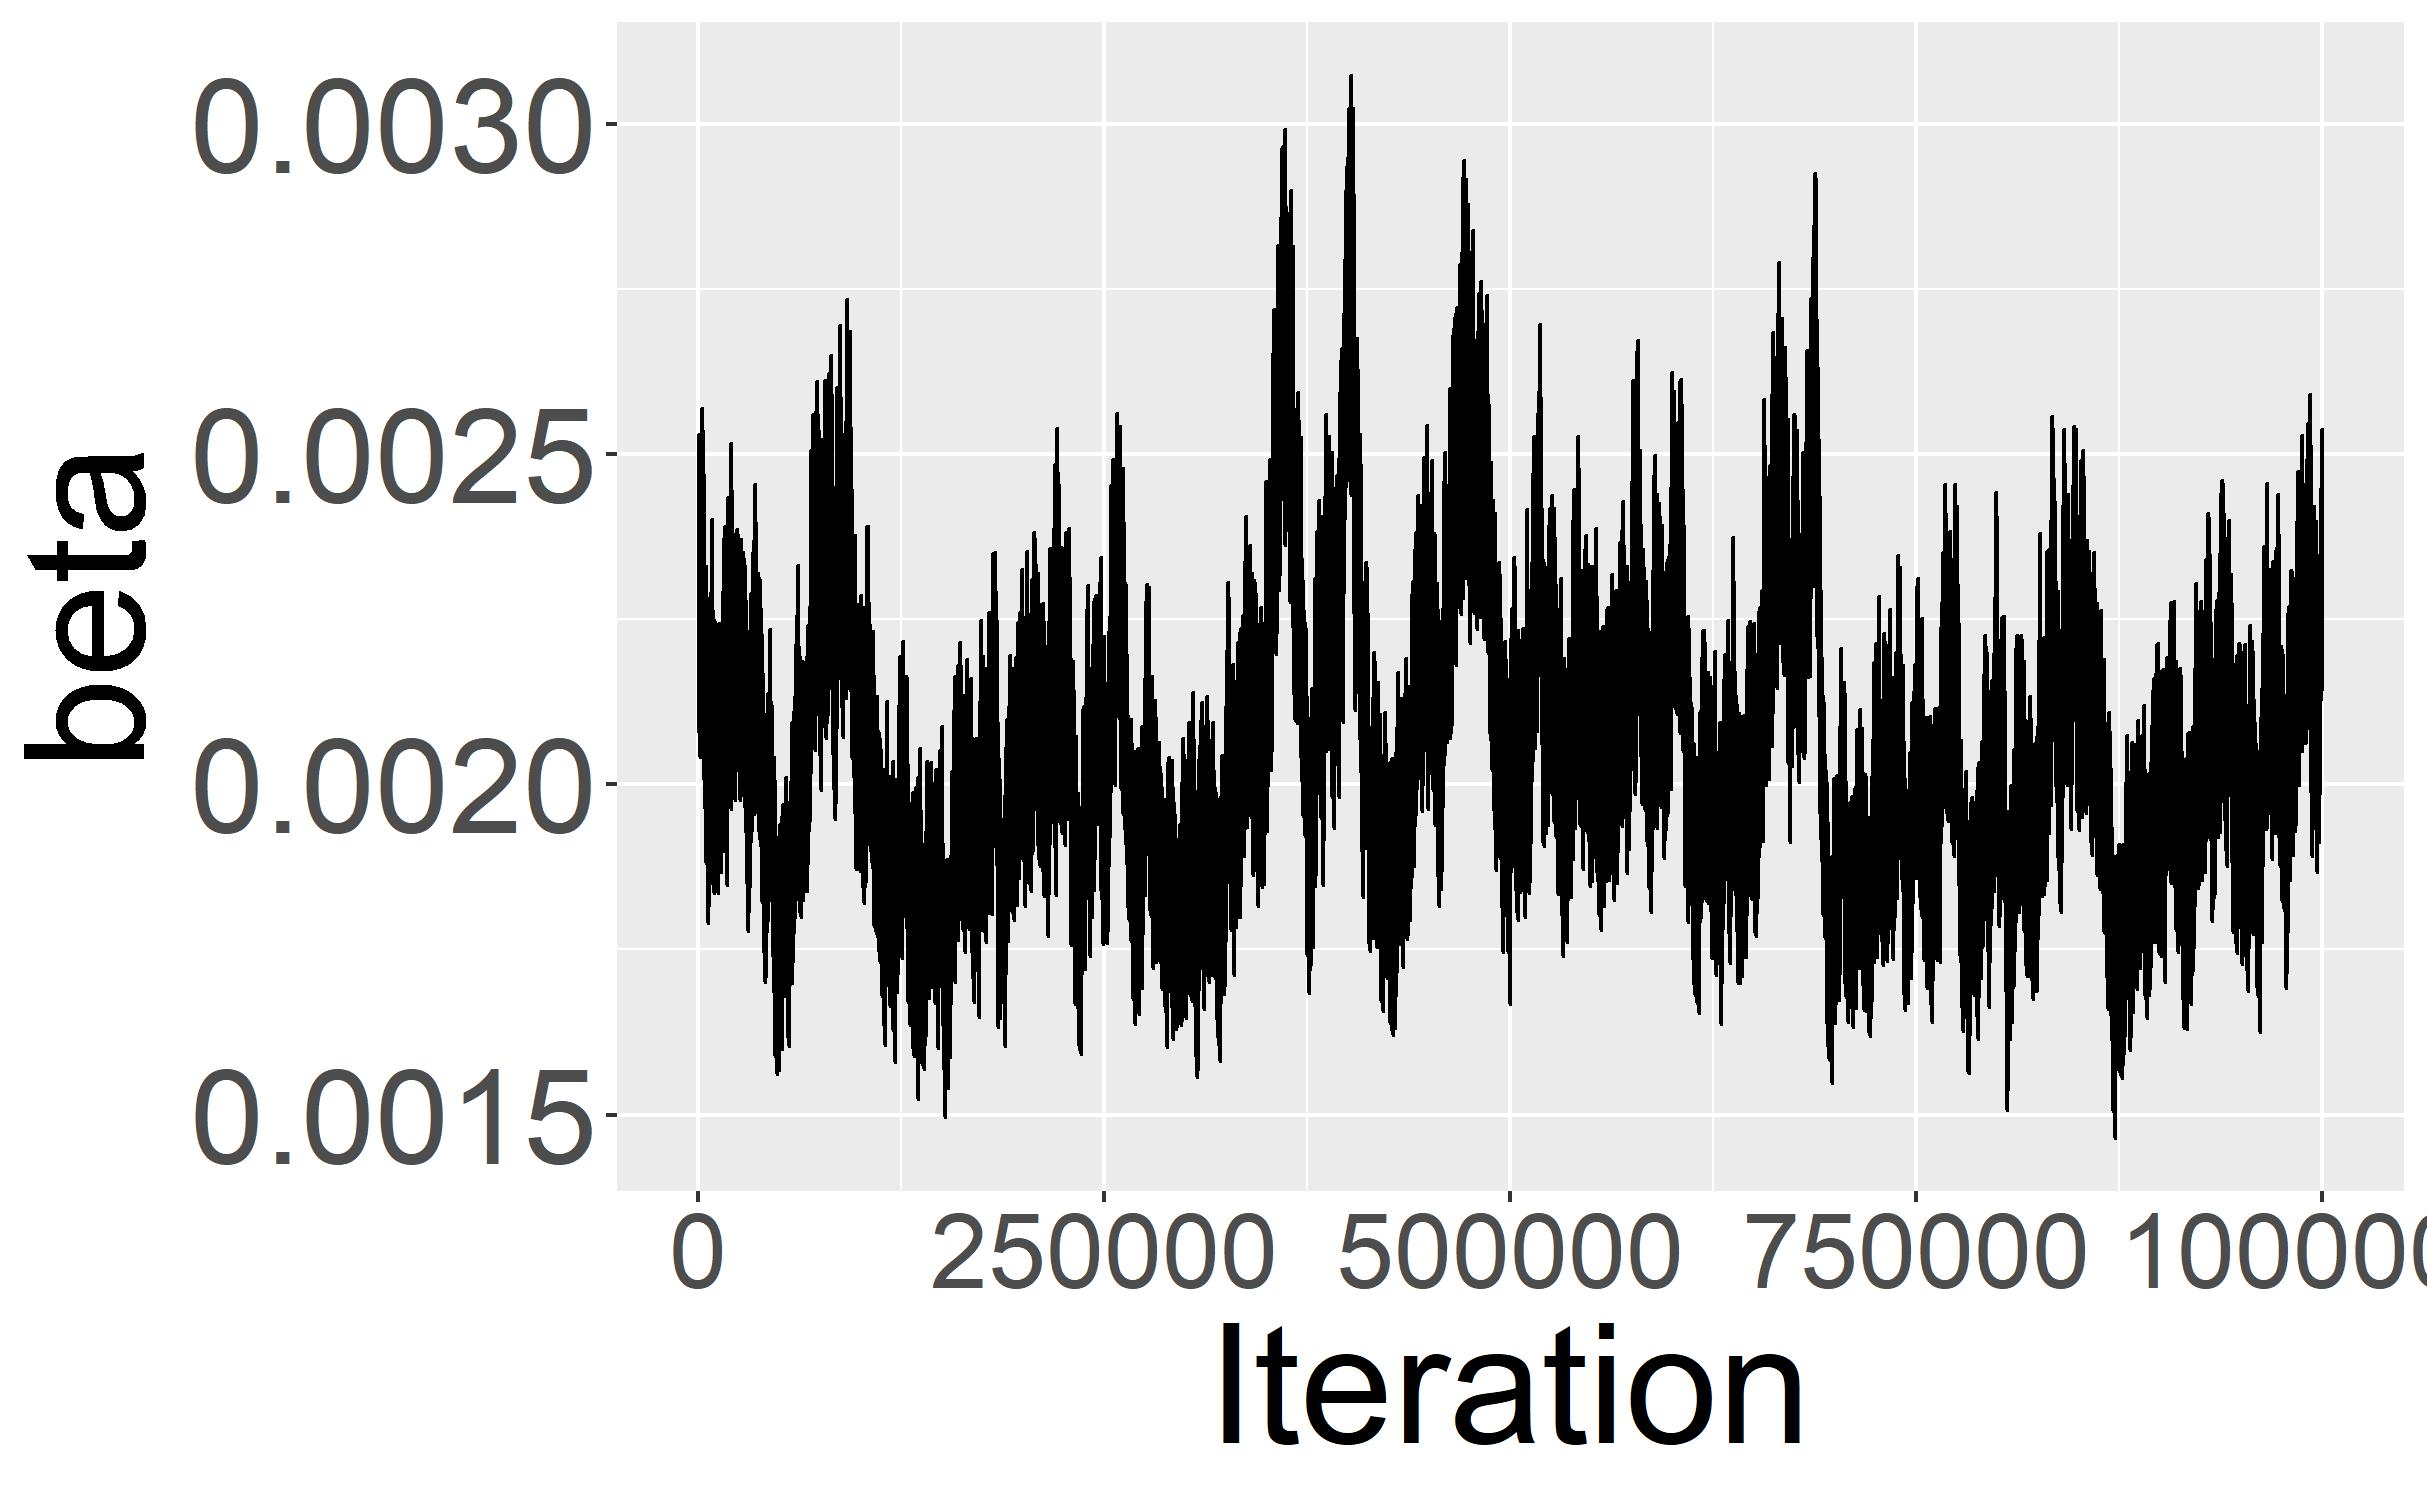
\includegraphics[width=0.49\textwidth]{E6_no_burn_beta_tp_single.jpg}
			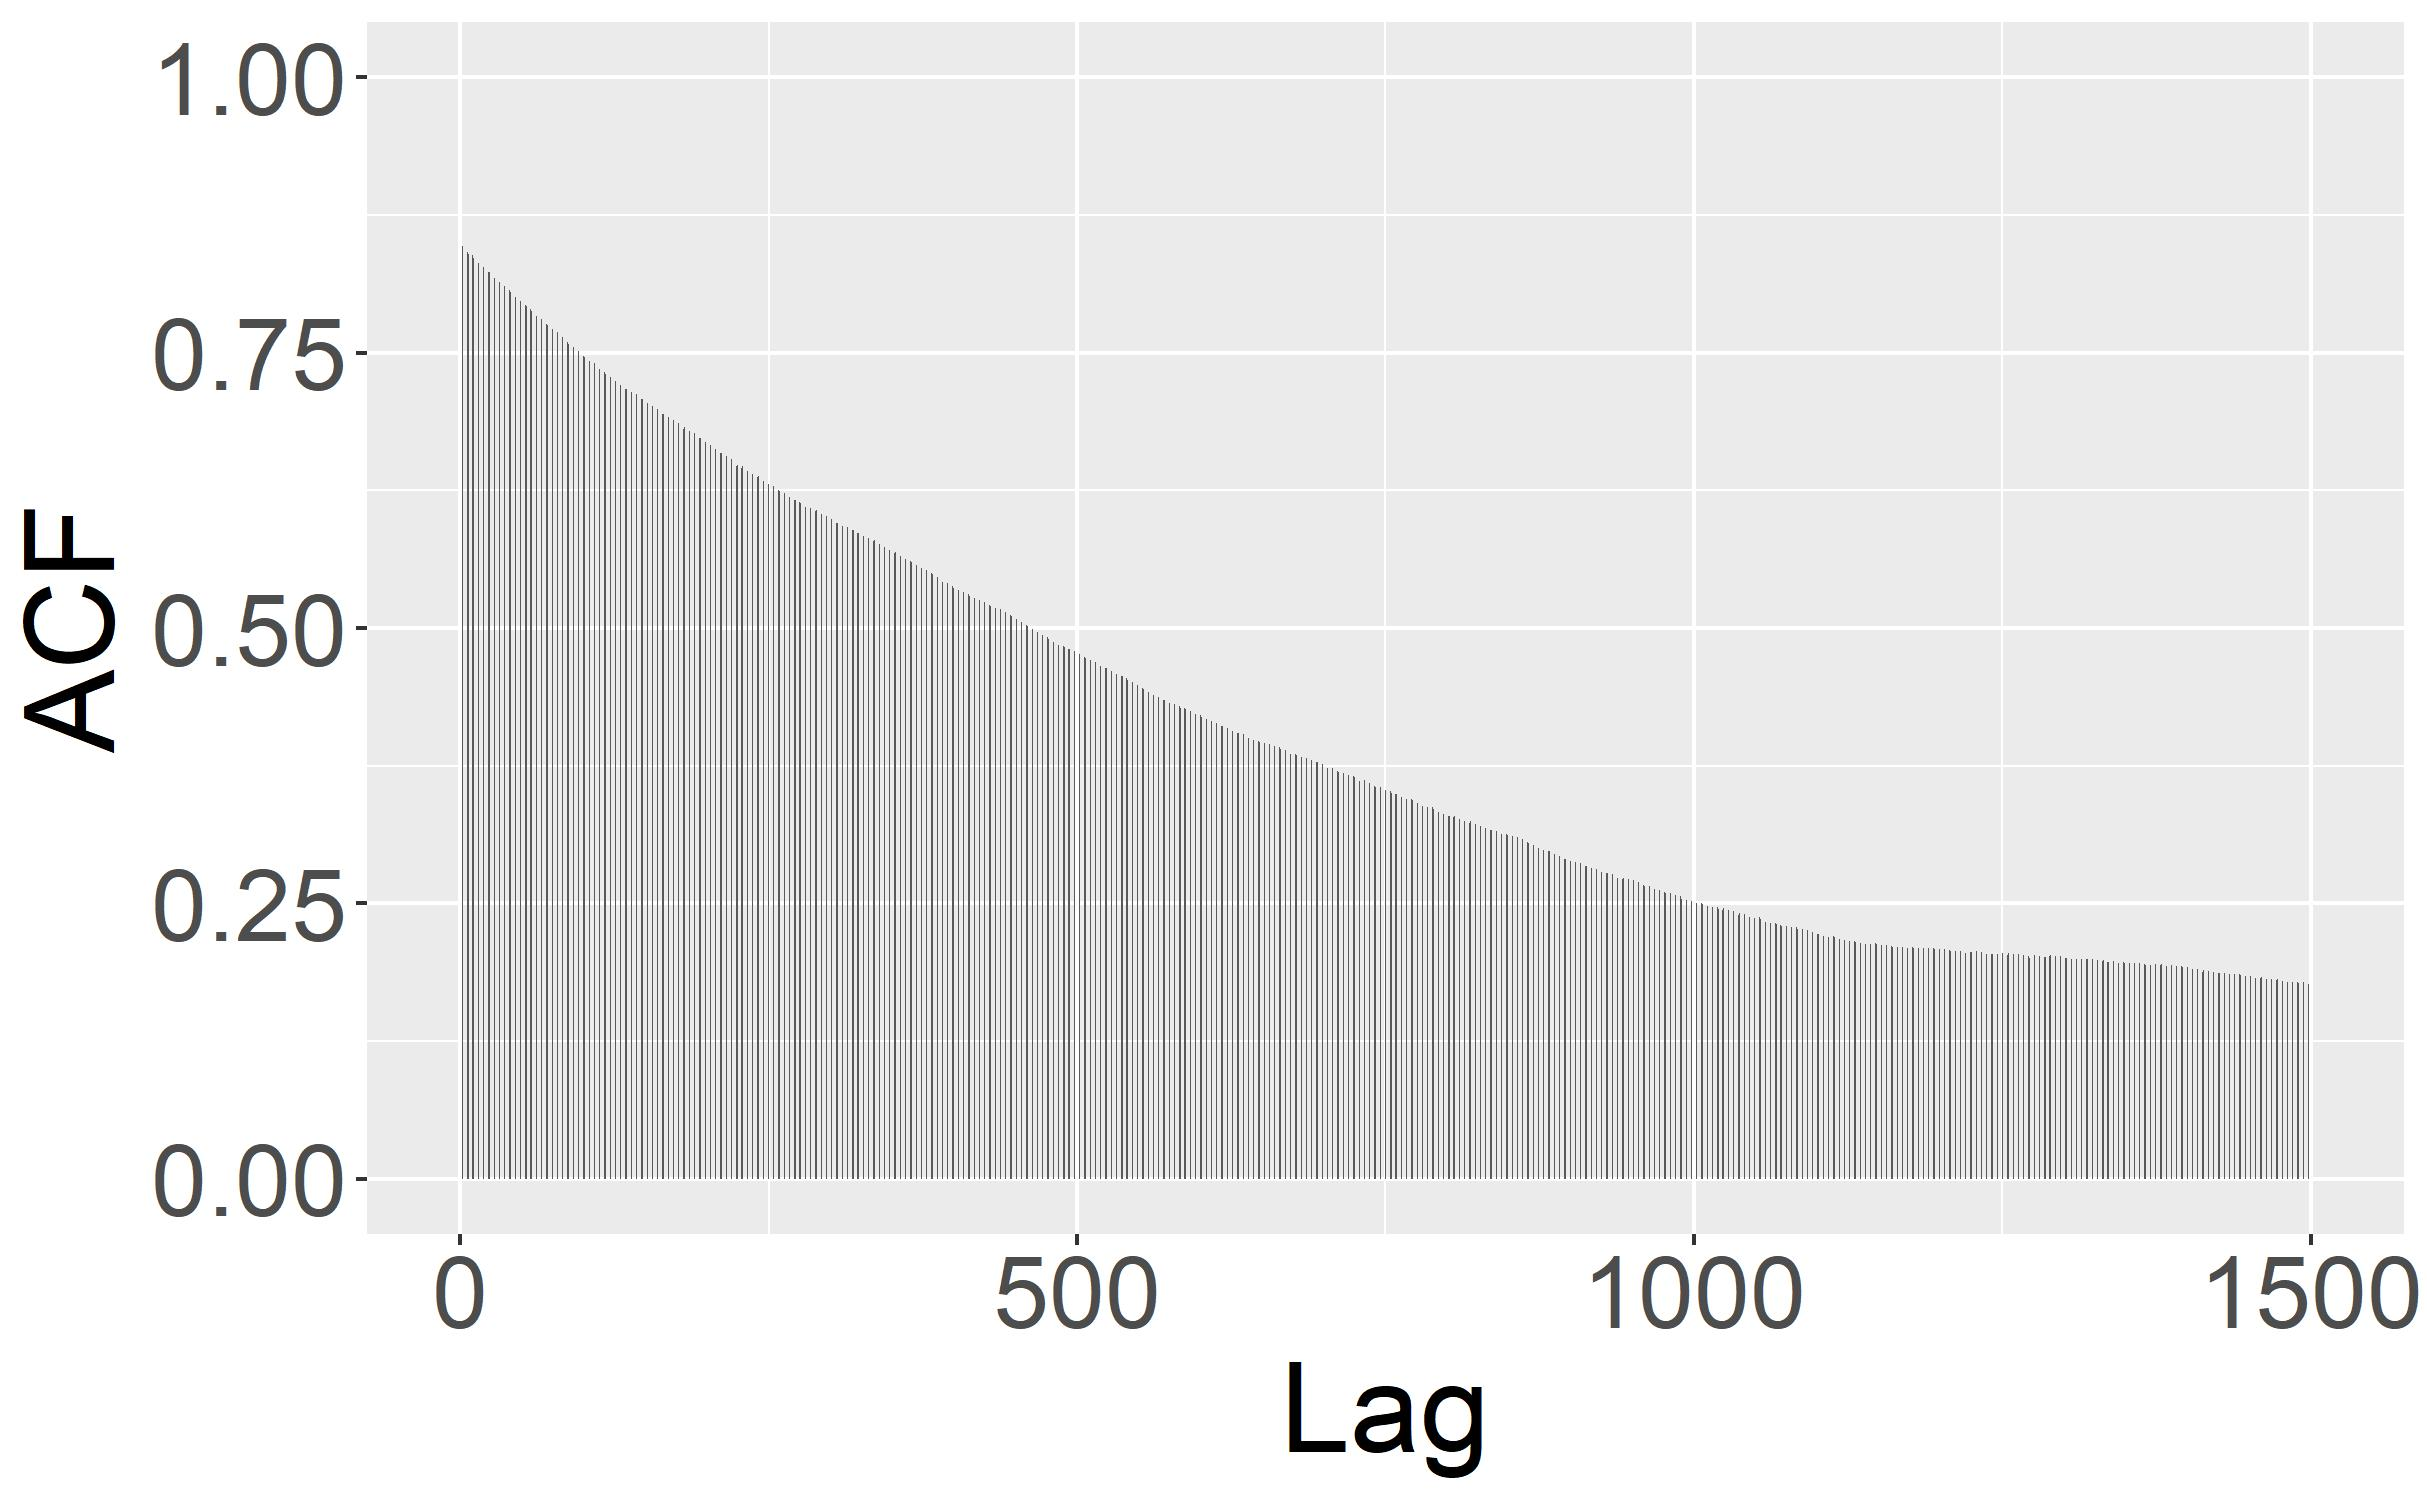
\includegraphics[width=0.48\textwidth]{E6_burn_beta_acf_single.jpg}
			\caption{SSU DA-MCMC}
			\label{fig:E6_no_burn_beta_tp_single}
		\end{subfigure}
		\caption{Traceplot and ACF of our DA-MCMC and a SSU DA-MCMC for $\beta$.}
		\label{fig:E6}
	\end{figure}
	
	
	\begin{table}
		\centering
		\begin{tabular}{ c|cc}
			Parameter & DA-MCMC & SSU DA-MCMC \\ 
			\hline
			$\beta$ & 0.20 & 0.01 \\ 
			$\gamma$ & 0.19 & 0.01 \\ 
			$R_0$ & 0.38 & 0.05 \\
			\hline
		\end{tabular}
		\caption{ESS/sec for our DA-MCMC and the SSU DA-MCMC.}
		\label{tab:E6}
	\end{table}
	
	
\end{frame}


\begin{frame} \frametitle{2013-2016 Ebola Pandemic in Western Africa}  
	\begin{itemize}
		\item Highly contagious virus, $>10000$ victims during the 2013-2016 pandemic in Western Africa.
		\item Weekly infection counts per province (Gueckedou).
		\item $n =$ 290,000; $\rho = 0.1$ (acceptance rate: 0.21)
		\item 1e6 iterations, 470 ESS.
	\end{itemize} 
	
	\begin{figure}
		\centering
		\begin{subfigure}[b]{0.32\textwidth}
			\centering
			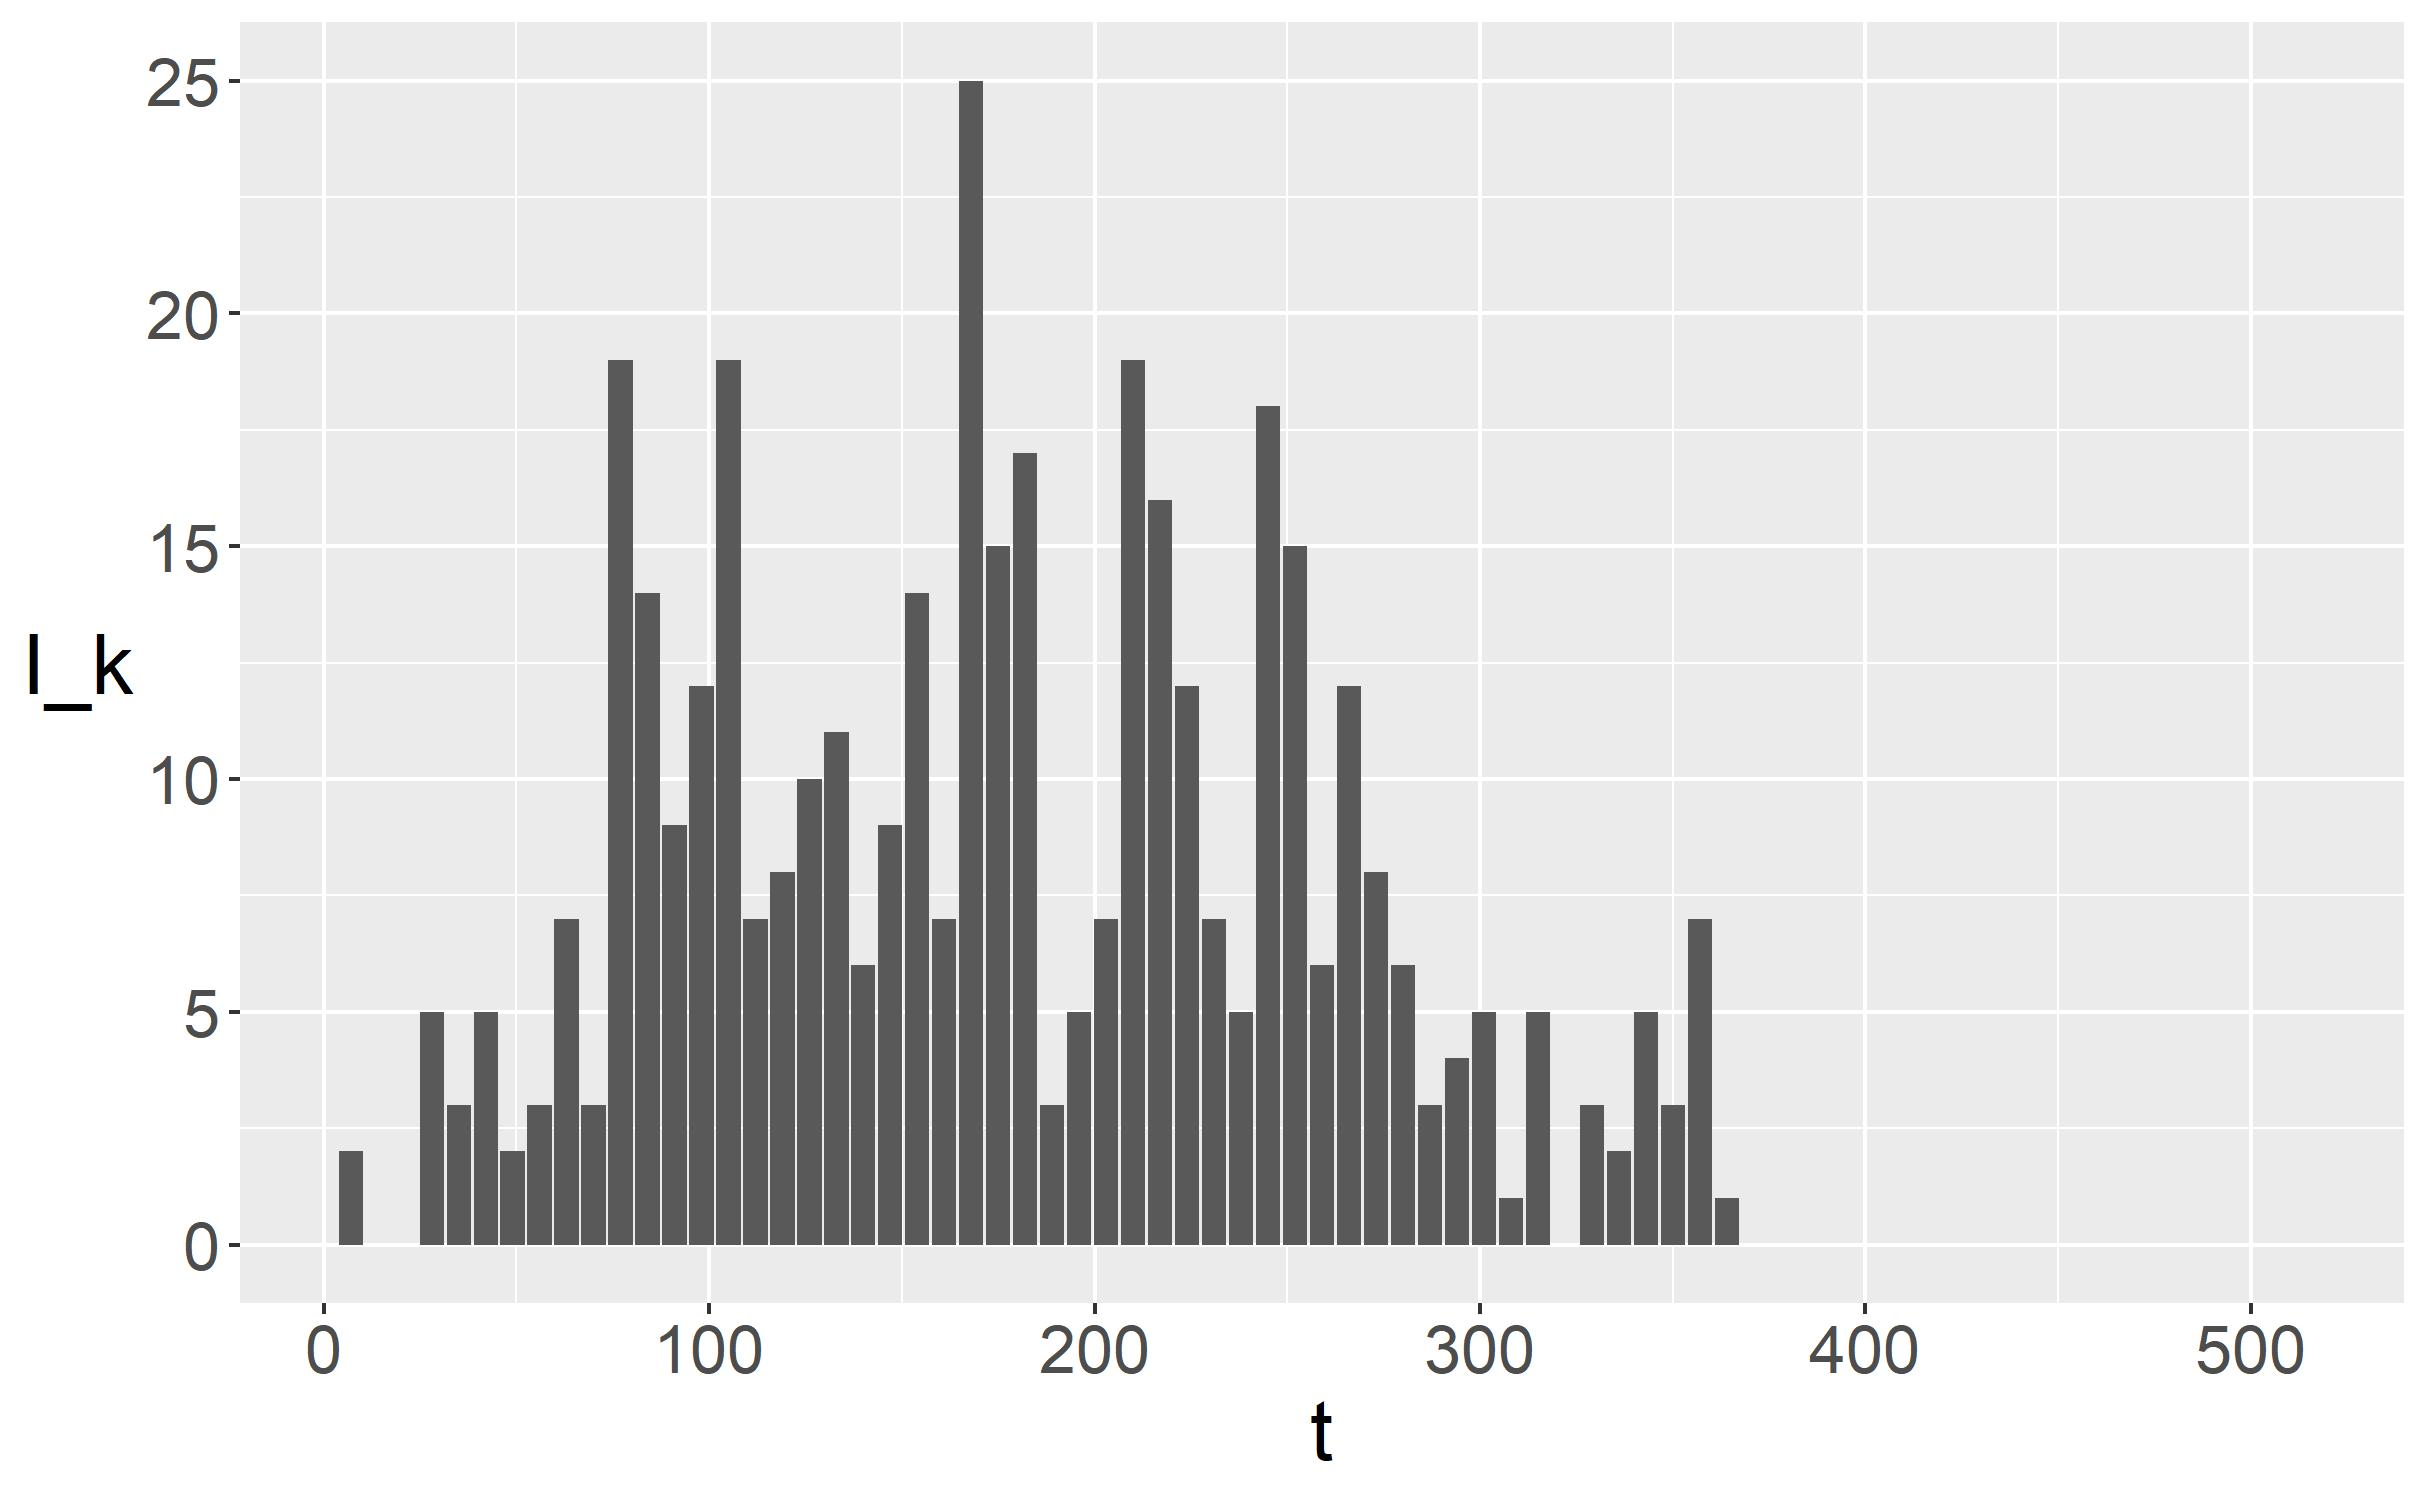
\includegraphics[width=\textwidth]{observed_data}
			\caption{Observed data}
		\end{subfigure}
		\hfill
		\begin{subfigure}[b]{0.32\textwidth}
			\centering
			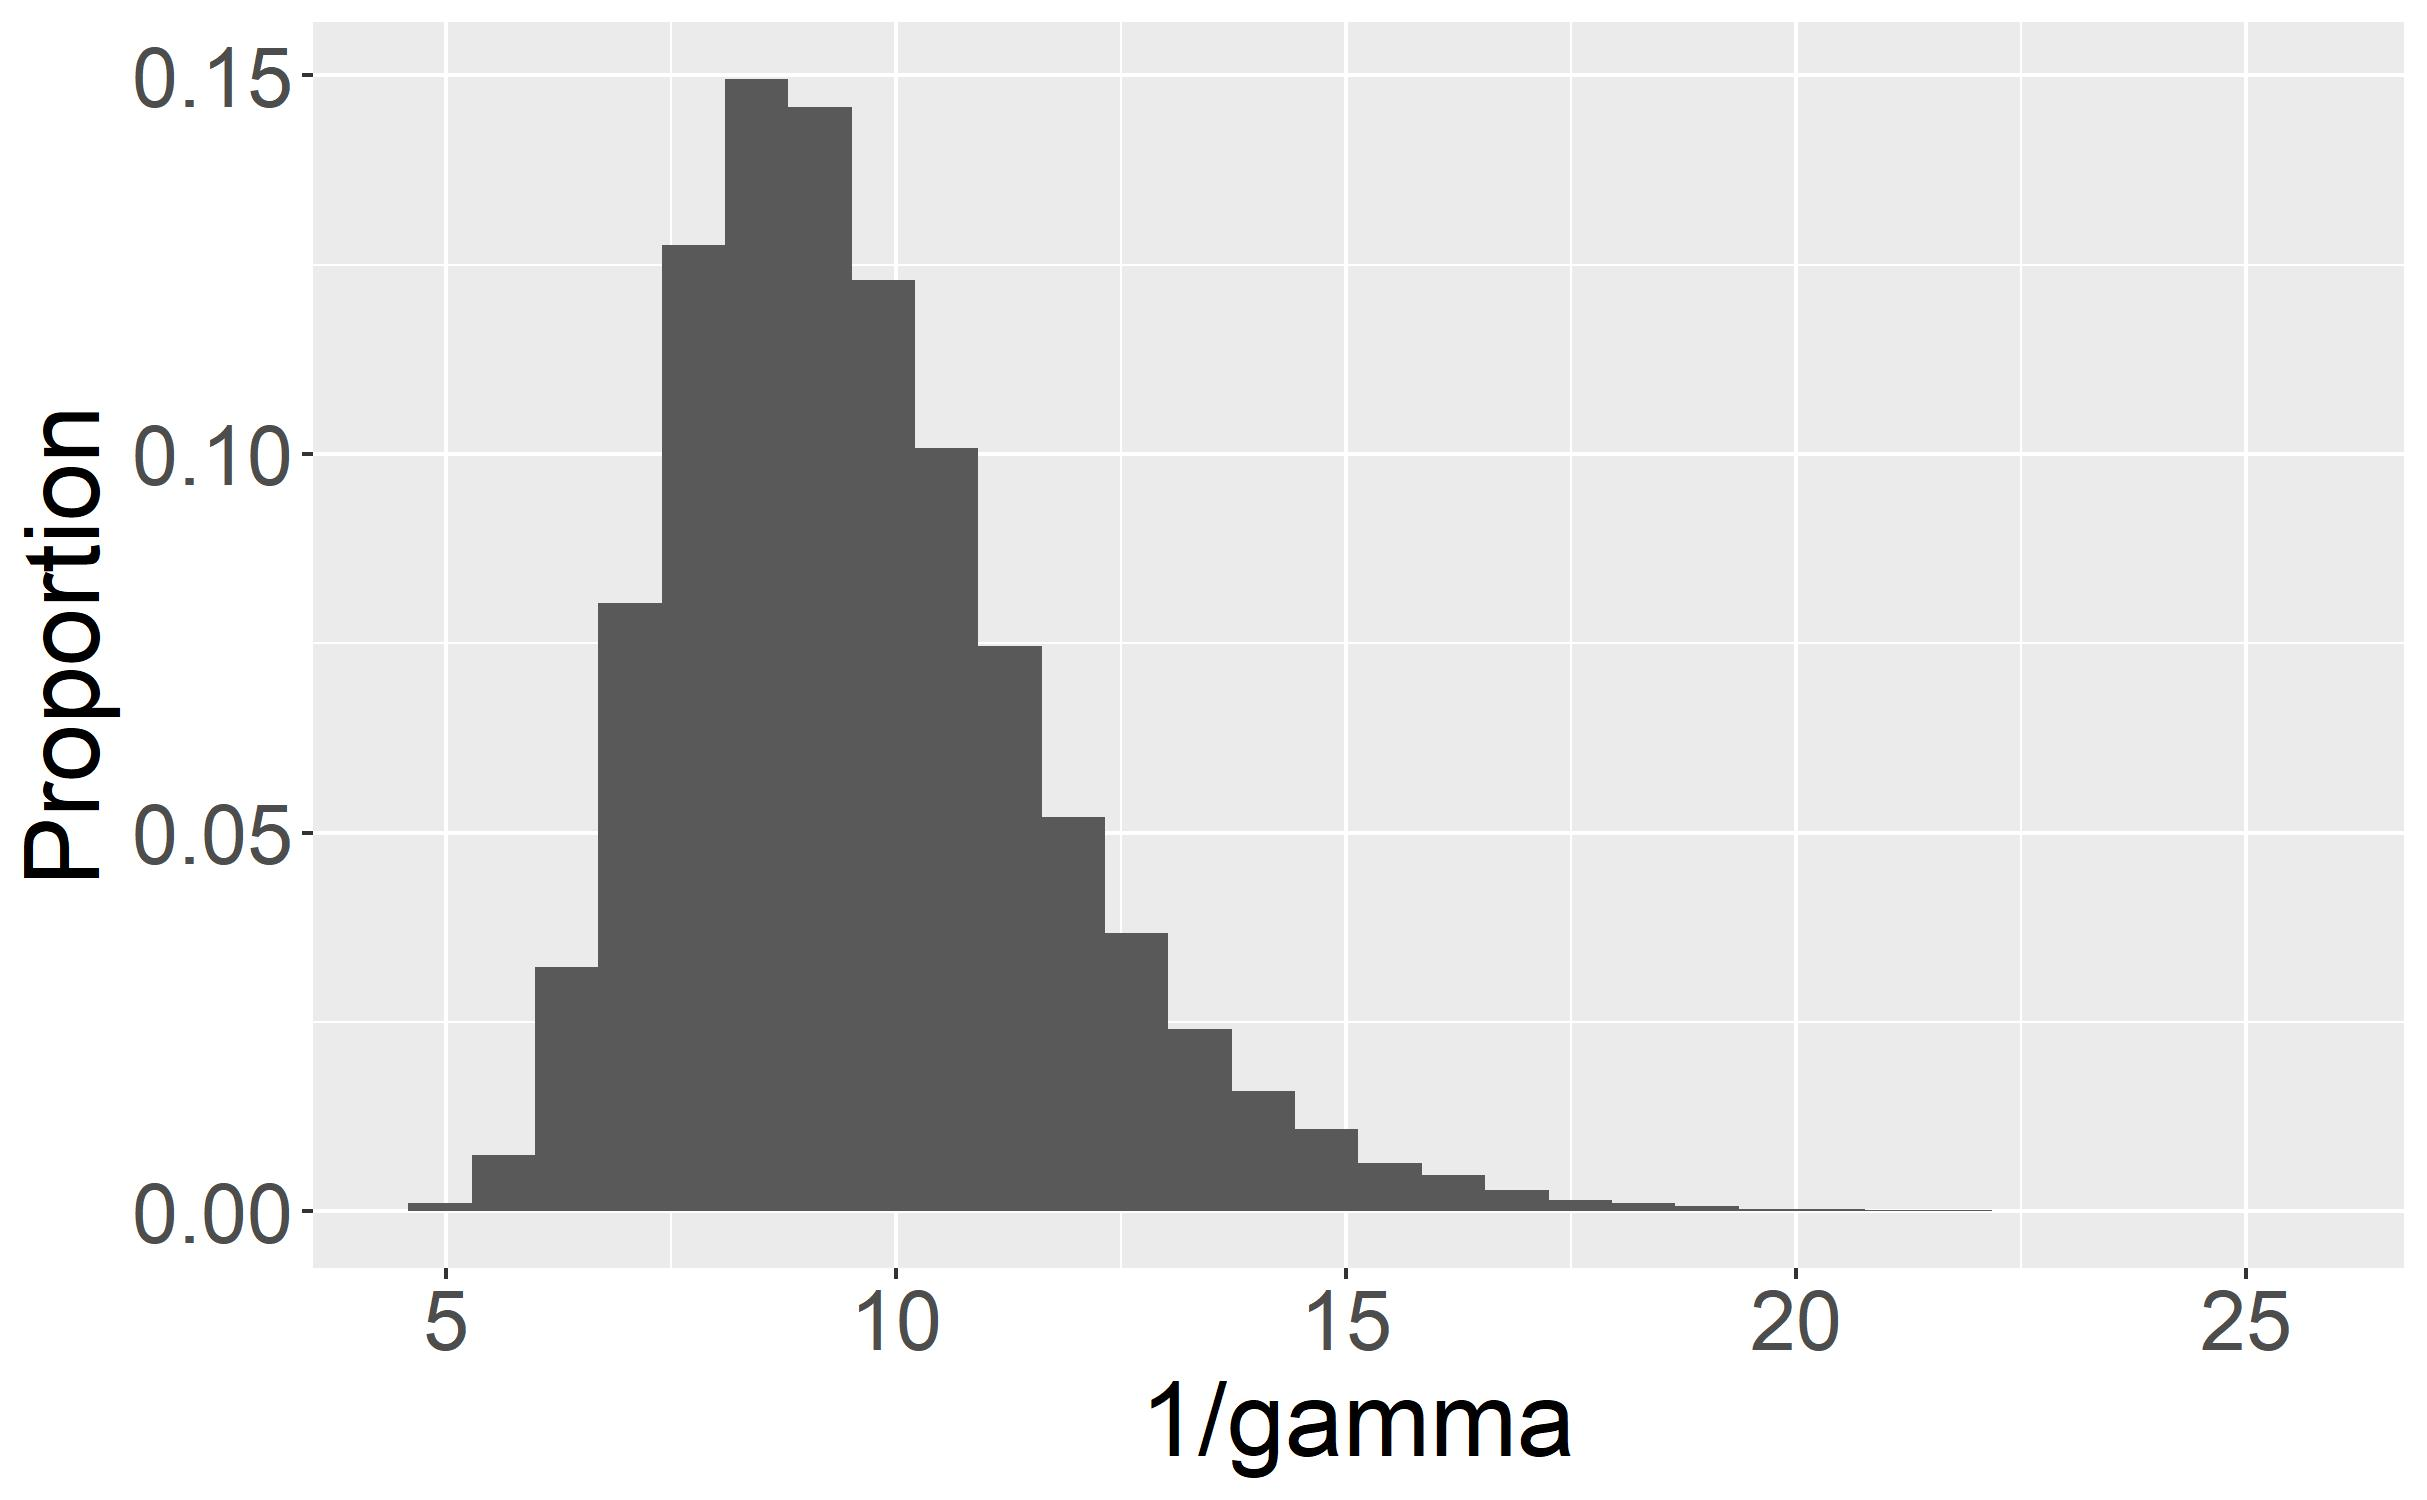
\includegraphics[width=\textwidth]{E5_expected_infection_length_hist}
			\caption{Posterior distribution}
		\end{subfigure}
		\hfill
		\begin{subfigure}[b]{0.32\textwidth}
			\centering
			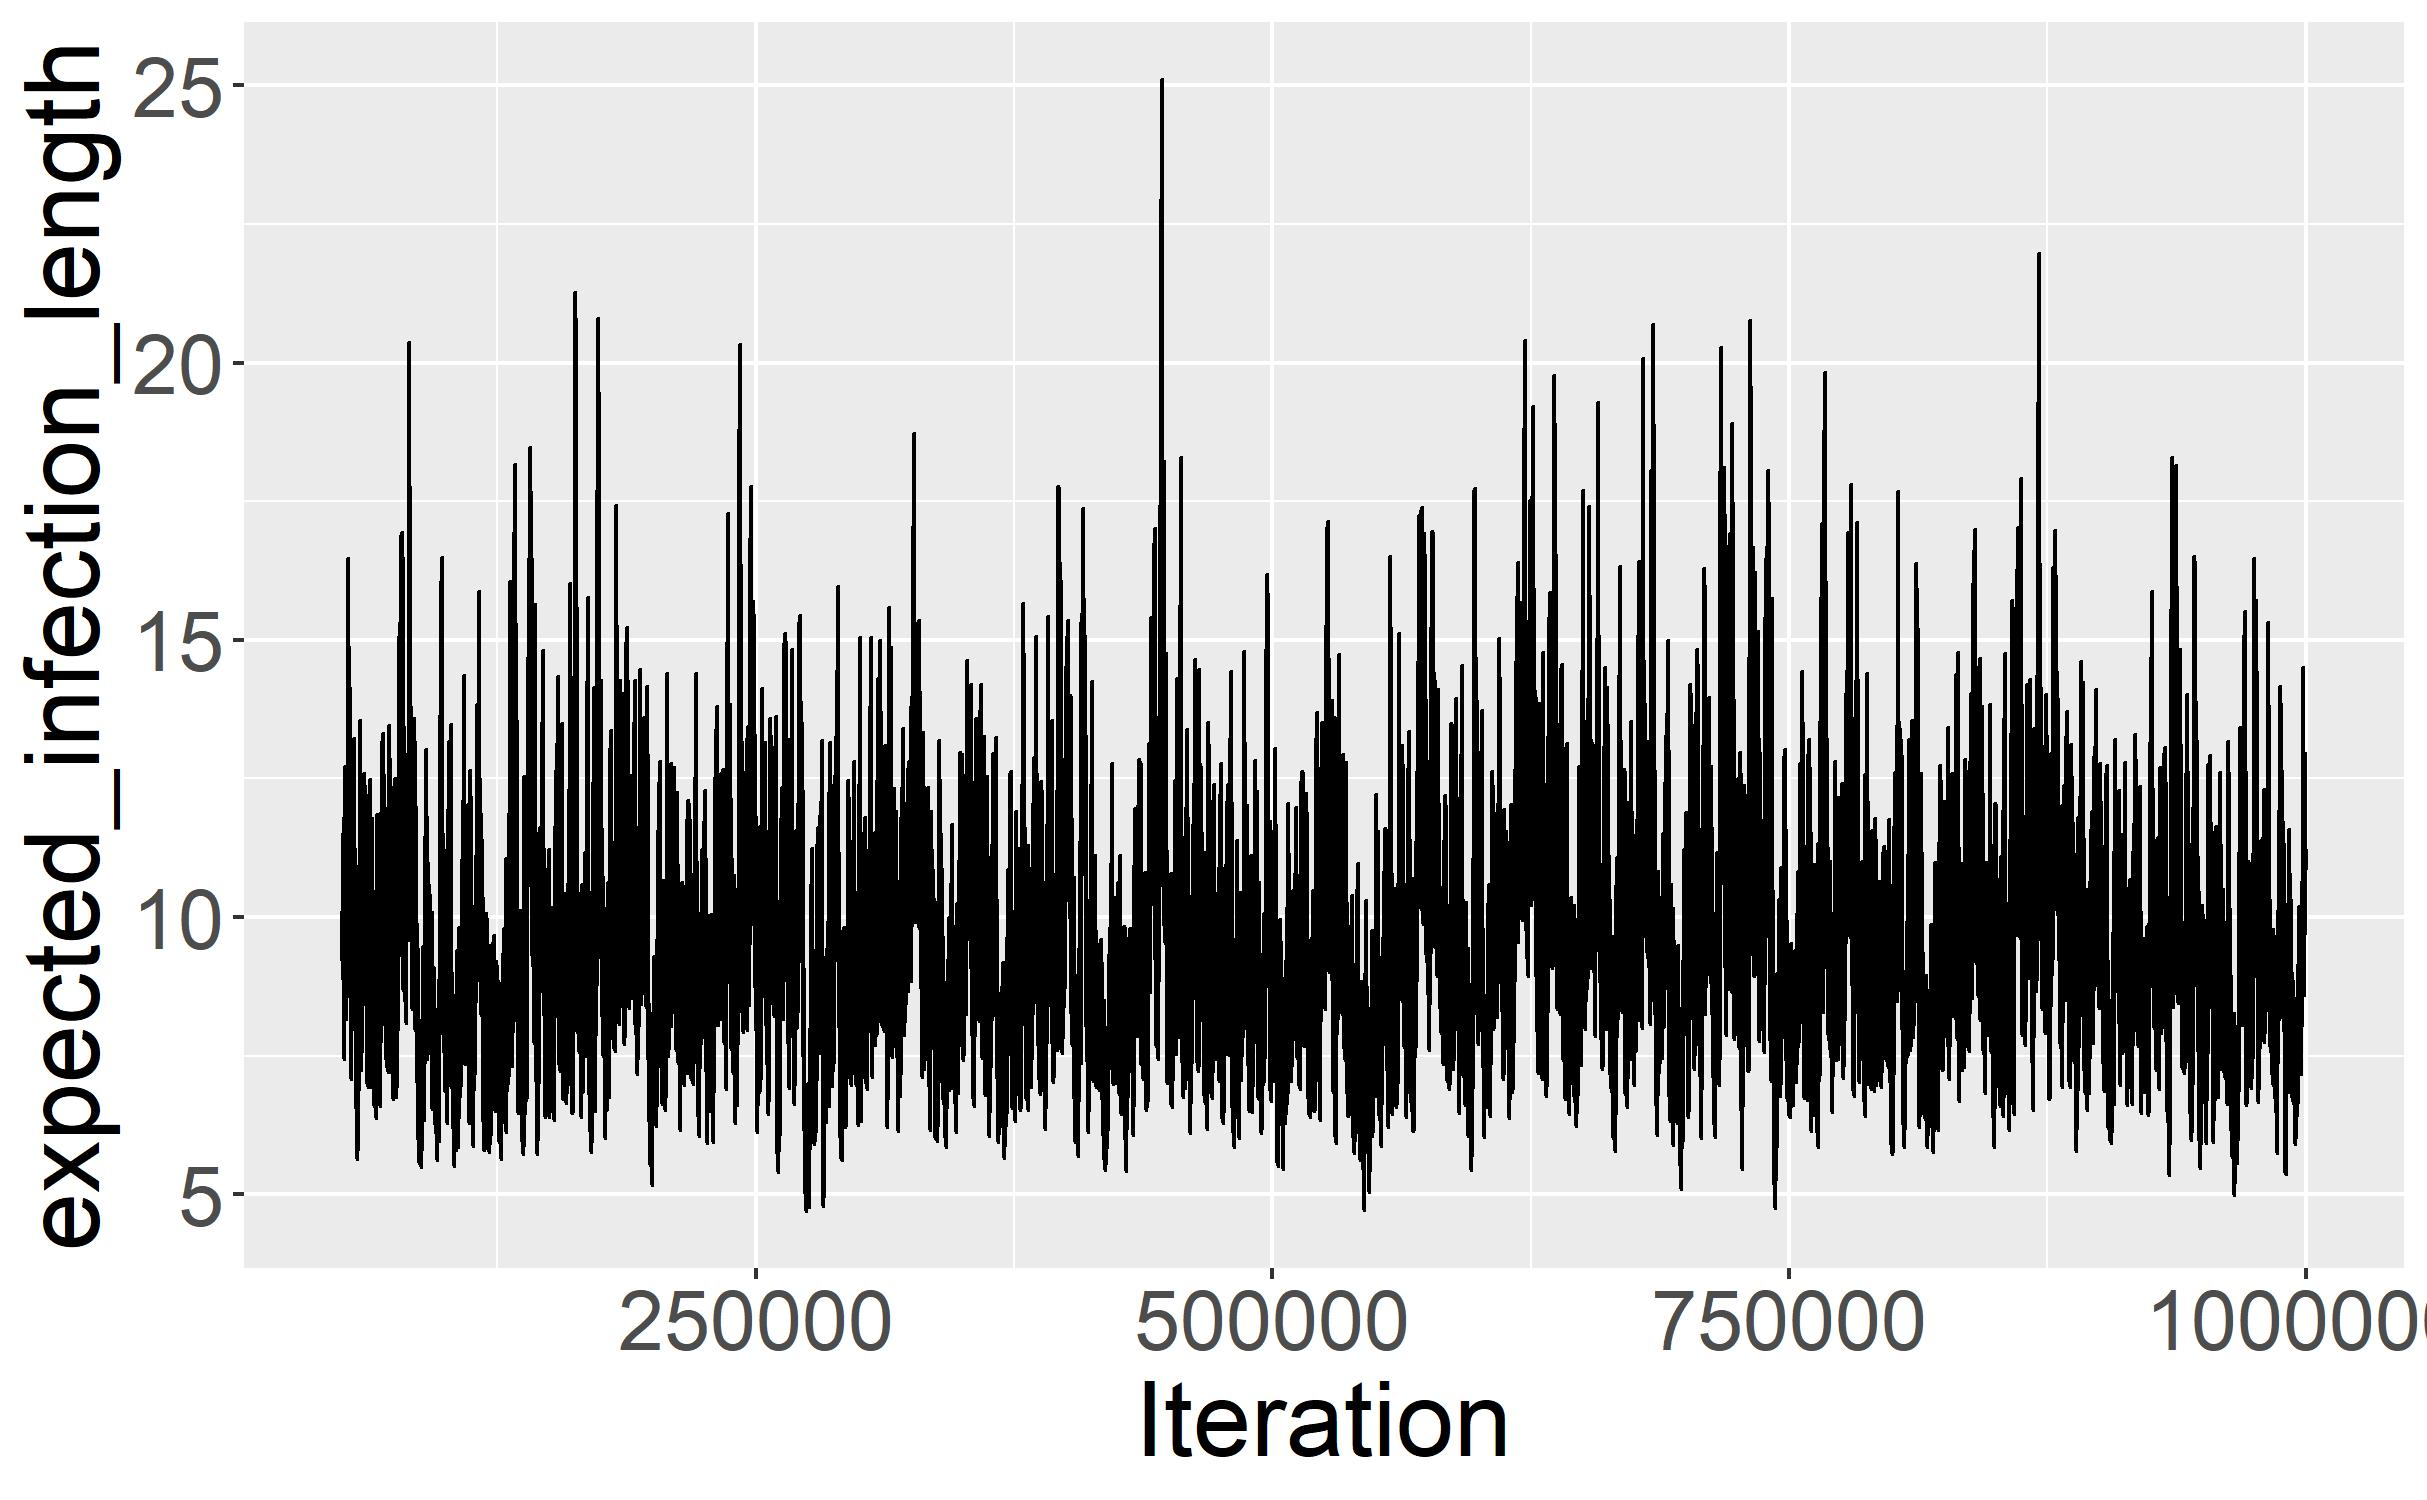
\includegraphics[width=\textwidth]{E5_expected_infection_length_tp}
			\caption{Traceplot}
		\end{subfigure}
		\caption{Observed data for the Gu\'eck\'edou prefecture and posterior distribution and traceplot of the expected infection length ($\gamma^{-1}$).}
		\label{fig:ebola}
	\end{figure}
	
	
\end{frame}


\begin{frame} \frametitle{Extensions}  
	
	We have extended the PD-SIR to
	\begin{itemize}
		\item non-Markovian SIR,
		\item SIR with heterogeneously mixing population.
	\end{itemize}

	I am mentoring a student who works on 
	\begin{itemize}
		\item SIR with time varying infection rate.
	\end{itemize}

	I plan to work on the following problems
	\begin{itemize}
		\item under-reporting e.g.\ $\tilde{I}_k \sim Bin(I_k, \kappa)$,
		\item IR approximation to the SIR (small pandemic in large population, e.g.\ Ebola) $\Rightarrow$ $I(t)$ is a linear birth-death process,
		\item applying our DA-MCMC to other processes where we observe incidence data (as opposed to prevalence data).
	\end{itemize}
	
\end{frame}



\begin{frame} \frametitle{Conclusion}  
	
	
	Our DA-MCMC is an efficient algorithm for exact Bayesian inference for the stochastic SIR with infection incidence data.	
	\begin{itemize}
		\item carefully designed surrogate process: efficient and fast.
	\end{itemize}
	
	The combination of (i) the agent-based formulation and (ii) the PD-SIR provides a unified inferential framework for the SIR with
	\begin{itemize}
		\item non-Markovian dynamics,
		\item a heterogeneously mixing population,
		\item a time varying infection rate.
	\end{itemize}
	
\end{frame}




\begin{frame} \frametitle{Extension -- Arbitrarily Distributed Infection Periods}
	
	\begin{itemize}
		\item Weibull distribution is more plausible for infectious periods.
		\item Dropping the assumptions of exponentially distributed infectious periods makes the process \textit{Non-Markovian}.
		\item Yet, the likelihood still has a closed form!
		\item PD-SIR with
		$$z^R_j | z^I_j \sim z^I_j + Weibull(.)$$
	\end{itemize} 
	
\end{frame}


\begin{frame} \frametitle{Extension -- Heterogeneously Mixing Population}
	
	\begin{itemize}
		\item Severo (1969) proposes to substitute the population-level infection rate of the SIR
		$$\mu_{pop}(t) =  \beta S(t) I(t)$$
		with 
		$$\bar{\mu}_{pop}(t) = \beta S(t)^{1-b} I(t), \quad b \in [0,1]$$
		to model a heterogeneously mixing population.
		\item The corresponding individual-level infection rate is 
		$$\bar{\mu}(t) = \dfrac{\bar{\mu}_{pop}(t)}{S(t)} = \beta S(t)^{-b} I(t)$$
		\item PD-SIR with
		$$\mu_k = \tilde{\mu}(t_{k-1}) = \beta S(t_{k-1})^{-b} I(t_{k-1}).$$
	\end{itemize} 
	
\end{frame}

\begin{frame} \frametitle{Extension -- Time-varying Infection Rate $\beta(t)$}
	
	\begin{itemize}
		\item $\beta \sim GP(.)$ (Kypraios, 2018)
		\begin{itemize}
			\item expensive: invert a matrix of order $n\times n$ each iteration
		\end{itemize}
		\item Random walk: $\Delta(\beta)_k \sim N(0, \sigma^2)$
		\begin{itemize}
			\item multivariate normal prior $\Rightarrow$ elliptical slice sampler
		\end{itemize}
		\item Locally adaptive: $\Delta(\beta)_k$ follows a Laplace or HS distribution (Faulkner \& Minin, 2018)
		\begin{itemize}
			\item accommodates sudden variations in $\beta$.
		\end{itemize}
		
	\end{itemize} 
	
\end{frame}


\begin{frame} \frametitle{Uniform Ergodicity -- Minorizing $P_\theta$}
	
	The density of the Gibbs kernel $P_\z$ corresponds to the product of the two gamma densities
	$$Ga\left(\beta; a_{\beta} + n_I, b_{\beta} + \int S(t)I(t)dt\right)Ga\left(\gamma; a_{\beta} + n_R, b_{\beta} + \int I(t)dt\right)$$
	Since the sufficient statistics of $\Z$ are bounded:
	$$0 \le \int S(t)I(t)dt \le n^2t_{end}, \quad 0\le n_R \le n, \quad 0 \le \int I(t)dt \le n t_{end},$$
	each density possesses a positive minorization whose closed form we have derived.
	
\end{frame}




\begin{frame} \frametitle{Uniform Ergodicity -- Minorizing $P_\z$}
	
	The MH kernel $P_\z$ depends on the current latent data $\z$ only through the ratio $q(\z|\theta)/\pi(\z|\theta)$. 
	\begin{itemize}
		\item $q$ and $\pi$ can be bounded above and below away from $0$.
	\end{itemize}
	
	It is illuminating to observe that
	\begin{itemize}
		\item the contribution of the removal times in the numerator and the denominator cancel each other (generated from identical dynamics),
		\item the ratio of infections times' contribution 
		$$\prod_{k=1}^K \prod_{j\in \mathcal{I}_k}\dfrac{\beta I(t_{k-1}) \exp\{-\beta I(t_{k-1}) (z^I_j - t_{k-1})\}}
		{\beta I(z^I_l) \exp\{-\beta \int_{t_{k-1}}^{z^I_j} I(t)dt\}}$$
		will typically be close to $1$. 
	\end{itemize}
	
\end{frame}


\begin{frame} \frametitle{Three Types of Partially Observed Data}

exact removal times; prevalence infectious counts; incidence infection counts


\end{frame}

\end{document}